% --------------------------------------------------------------------------------
%                     __   __        _      _    _
%                     \ \ / /_ _ _ _(_)__ _| |__| |___ ___
%                      \ V / _` | '_| / _` | '_ \ / -_|_-<
%                       \_/\__,_|_| |_\__,_|_.__/_\___/__/
%
% --------------------------------------------------------------------------------
\newcommand{\classname}{extbook}
\newcommand{\innermargin}{3.8cm}
\newcommand{\outermargin}{5.4cm}
\newcommand{\bodyfont}{Century Supra A}
\newcommand{\headingfont}{Concourse 6 Caps}
\newcommand{\sansfont}{Concourse 3}
\newcommand{\scfont}{Century Supra A Caps}
\newcommand{\monospacefont}{Triplicate A}
\newcommand{\Footheadfont}{Concourse 4 Caps}
\newcommand{\footheadfont}{Concourse 4}
\newcommand{\titlepagename}{cn-titlepage}
\newcommand{\spacingvalue}{1.25}
\newcommand{\headsepvalue}{30pt}
\newcommand{\footskipvalue}{40pt}
\newcommand{\marginparsepvalue}{20pt}
\newcommand{\marginparwidthvalue}{90pt}


% --------------------------------------------------------------------------------
%                          _  _             _
%                         | || |___ __ _ __| |___ _ _
%                         | __ / -_) _` / _` / -_) '_|
%                         |_||_\___\__,_\__,_\___|_|
%
% --------------------------------------------------------------------------------
\documentclass[10pt]{\classname}
\usepackage[T1]{fontenc}
\usepackage[utf8]{inputenc}
\usepackage[italian]{babel}
%\usepackage[document]{ragged2e}
\usepackage{fontspec}
\usepackage{mlmodern}
\usepackage[stickstoo]{newtxmath}
\usepackage[all]{nowidow}
\usepackage{graphicx}
\usepackage{svg}
\usepackage[pdfa]{hyperref}
\usepackage{color}
\usepackage{makecell}
\usepackage{setspace}
\usepackage{parskip}
\usepackage[a4paper, inner=3.8cm, outer=5.4cm]{geometry}
\usepackage{listings}
\definecolor{dkgreen}{rgb}{0.1,0.5,0.1}
\definecolor{greengray}{rgb}{0.517,0.761,0.404}
\definecolor{orange}{rgb}{0.717,0.274,0.105}
\definecolor{blue}{rgb}{0.164,0.317,0.600}
\definecolor{background}{rgb}{0.990,0.990,0.990}
\lstset {
	frame=lrtb,
	language=java,
	aboveskip=0.7cm,
	belowskip=0.2cm,
	showstringspaces=false,
	columns=flexible,
	basicstyle={\small\ttfamily},
	numbers=none,
	backgroundcolor=\color{background},
	numberstyle=\tiny\color{dkgreen},
	keywordstyle=\color{blue},
	commentstyle=\color{greengray},
	stringstyle=\color{orange},
	breaklines=true,
	breakatwhitespace=true,
	tabsize=3
}

\font \bodyfontfs = "\bodyfont"
\font \sansfontfs = "\sansfont"
\font \scfontfs = "\scfont"
\font \monofontfs = "\monospacefont"
\font \Footheadfontfs = "\Footheadfont"
\font \footheadfontfs = "\footheadfont"

\usepackage{fancyhdr}
\pagestyle{fancy}
\fancyhf{}
\fancyhead[LE,RO]{\Footheadfontfs \nouppercase \leftmark}
\fancyfoot[CE,CO]{\footheadfontfs \thepage}
\renewcommand{\headrulewidth}{1.0pt}
\renewcommand{\footrulewidth}{1.0pt}
\renewcommand{\chaptermark}[1]{\markboth{#1}{}}

\newtheorem{thm}{Teorema}
\setlength{\tabcolsep}{0.5em} % for the horizontal padding
{\renewcommand{\arraystretch}{1.35}% for the vertical padding


\begin{document}
\setmainfont{\bodyfont}
\setsansfont{\sansfont}
\setmonofont{\monospacefont}

\include{\titlepagename}
%\title{Title}
%\author{Author}
%\maketitle

\setstretch{\spacingvalue}
\setlength{\emergencystretch}{0pt}
\pretolerance=150
\tolerance=250
\hbadness=150
\hfuzz=0pt
\setlength{\headsep}{\headsepvalue}
\setlength{\footskip}{\footskipvalue}
\setlength{\marginparsep}{\marginparsepvalue}
\setlength{\marginparwidth}{\marginparwidthvalue}

\tableofcontents

\let\oldtextsc\textsc
\renewcommand{\textsc}[1]{\oldtextsc{\scfontfs #1}}
\let\oldchapter\chapter
\renewcommand{\chapter}[1]{\setmainfont{\headingfont}\oldchapter{#1}\setmainfont{\bodyfont}}
\let\oldsection\section
\renewcommand{\section}[1]{\setmainfont{\headingfont}\oldsection{#1}\setmainfont{\bodyfont}}
\let\oldsubsection\subsection
\renewcommand{\subsection}[1]{\setmainfont{\headingfont}\oldsubsection{#1}\setmainfont{\bodyfont}}
\let\oldsubsubsection\subsubsection
\renewcommand{\subsubsection}[1]{\setmainfont{\headingfont}\oldsubsubsection{#1}\setmainfont{\bodyfont}}


% --------------------------------------------------------------------------------
%                     ___                             _
%                    |   \ ___  __ _  _ _ __  ___ _ _| |_
%                    | |) / _ \/ _| || | '  \/ -_) ' \  _|
%                    |___/\___/\__|\_,_|_|_|_\___|_||_\__|
%
% --------------------------------------------------------------------------------

\part{Security in Networking Protocols}

\chapter{Transmission Control Protocol internals}

\section{TCP Basis}

\subsection{Recap}

TCP is a protocol that has the following remarkable properties,

\begin{enumerate}
	\item it is \emph{connection-oriented}: before transmitting data, a
		connection must be established \--- this is different to what
		IP protocol does in network layer, since in IP protocol there
        lies no concept of connection, and messages are exchanged under the
        paradigm of \emph{packet switching}\footnote{In telecommunications,
        packet switching is a method of grouping data into packets that are
    transmitted over a digital network. Packets are made of a header and a
payload. Data in the header is used by networking hardware to direct the packet
to its destination, where the payload is extracted and used by an operating
system, application software, or higher layer protocols. Packet switching is
the primary basis for data communications in computer networks worldwide. };
	\item it is \emph{reliable}: it assures all segments are correctly
		delivered through use of \emph{ACK} mechanism, and \textbf{at
		most once} \--- again, this is different to IP layer, since IP
        packets are just sent one after the other, unreliably, and there is no
        guarantee that they will be delivered, let alone in their correct
        ordering;
	\item it offers a \emph{sliding window} mechanism for congestion control
		and stream control. This assures read and send buffers are
		well-optimized in both sender and receiver \--- this feature is
		much important since it allows fine-tuning the connection and
		avoiding waste of resources;
	\item it is \emph{byte-oriented}: the byte stream is fragmented into
		multiple segments, and composed again after getting to
		destination \--- in this manner, huge payloads can be reliably
		delivered in multiple segments, each one having the correct
		order to the application. Application has the necessary information
		to easily reconstruct the correct ordering of the acquired 
		information.
\end{enumerate}

Ultimately, TCP allows creating connections between application processes,
offering multiple services to the upper layers. Connections are possible thanks
to the four above characteristics of the TCP layer.

\subsubsection{Sockets}

The TCP makes use of \emph{sockets} abstraction as a way of serving data to the
above application layer. The logical structure is the following one: there are
two entities, the client and the server. The client first authenticates to the
server; the server then opens a connection and the client executes the
subsequent send-receive loop. Both server and client need to create a
\emph{socket} $s$ (a UNIX-like file abstraction), that can be used to send and
receive data. Client connect $s$ to \texttt{IP-srv}, \texttt{port-srv}, while
the server operates a similar procedure on its own sockets. Each socket is then
bound to a specific IP address and a specific \emph{port number}, according to
the just-created connection specifics.

The communication takes place on $s$ by means of an application protocol, with
applications exchanging data each other. The connection is said to be
\emph{reliable}: losses and packet loss are carefully managed by the TCP
protocol, and segments\footnote{\emph{Segments} refer to the particular kind of
package that TCP protocol exchange. Usually, in literature one could find the
term package referring to TCP segments; while this is not fully correct, it may
be acceptable when there is no ambiguity.} are collected in the very same order
as they are sent.

A very simplified pseudo-code at client's side for TCP is as follows,

\begin{verbatim} int s; s := socket(...); 
connect(s, IP-srv, port-srv,...); 
...
send (s, msgl, ...); 
... 
msg2 := receive(s,...); 
... 
\end{verbatim}

where the notation \emph{...} denotes possibly code in between two
instructions. In the above code, a client wants to send data to a remove server
having a specific IP address and a port number. The client first creates a
socket, then connects it to the server IP address and to the corresponding port
number. After connection has been established, the client can subsequently
invoke \texttt{send()} to command TCP layer to deliver desired data to the
other end. To the very same socket, data can be received as well: by invoking
\texttt{receive()} the client can successfully retrieve eventual data sent by
the server. Socket acts as an \emph{abstraction} for the application layer, for
which a socket can be simply thought as a \textbf{data sink} or \textbf{data
source}.

At server side, the logical structure is quite different. A server creates
a socket \texttt{s1}, chooses a port number to bind to that socket (usually a
standard one), then it declares \emph{willingness to accept connections} on
\texttt{s1}, and finally it awaits for connection requests on \texttt{s1}. Upon
receiving a connection request, the server handles it by creating
\emph{another} socket \texttt{s2} and managing the connection on this newly
generated socket, this time with a different port number. 

Basically, it creates two different sockets: the first is kept alive to accept
new connections, and the second one is created on-demand, and it is required to
actually manage the connection. A \emph{different} socket is required for each
connection. A server usually remains on \emph{sleep} until a connection is
requested, awaiting a request on the main socket.

\begin{verbatim} 
s1 := socket(...);
bind(s1, portsrvm ...);
listen(s1,...);
s2 := accept(s1,...); // another socket
... 
msg1 := receive(s2,...);
...
send(s2,msg2,...);
... 
\end{verbatim}

Details of the above code largely depend on the platform on which the server is
operating.

\subsection{TCP Implementation}

TCP layer is built \emph{on top} of the IP layer. Since there are many differences
between TCP and IP, set aside their abstraction layer, TCP should be properly
built to manage IP differences and quirks. 

IP protocol operates between \emph{nodes}: it is \emph{connectionless},
\textbf{unreliable}, and is \emph{mes\-sa\-ge--o\-rien\-ted}. The \textbf{Maximum
Transmission Unit} size of an IP packet is $MTU = 64KB$: this implicitly means
a TCP segment can never be greater than the MTU, because a TCP segment is
carried \emph{inside} an IP packet.

In TCP, communication happens to be \textbf{bidirectional}, with a pattern that
depends on the application protocol. The send\---receive patterns heavily depends
on the application itself \-- browser-related send\---receive sequences are
very different from, let's say, an e-mail client send\---receive sequence.
There is no guarantee that two different application protocols will exchange a
similar amount and kind of TCP messages, let alone the very same ones.

As already mentioned, TCP layers communicate between themselves in terms of
\emph{segments}. A segment is a single \emph{message between TCP layers}, and
contains a \emph{TCP header} and \--- eventually \--- data, that is said to be
\emph{payload}. The difference between information in header and information in
payload is that the first one is strictly required by the TCP layer, while the
second one is information required by the application layer. The latter may be
absent in some segments.

Payload in fact can either be $0$ bytes long or carry some information (wanted
by the application layer). \emph{A TCP segment must be small enough to fit in a
single IP packet}, hence IP header and TCP segment size should be no greater
than $64KB$, the MTU of an IP packet.

Since a packet is composed by a IP header, whose payload is a TCP segment, and the
TCP segment is in turn composed by a TCP header, followed by eventual
application data, the shape of a packet plus its segment can be summarized as
follows,

\begin{verbatim}
| IP header | TCP header |  Payload ***  |
\end{verbatim}

Usually, IP header size is usually $20$ bytes, as well as TCP
header that is $20$ bytes. The IP datagram can be greater up to $64KB$, with
the first $40$ to $50$ bytes reserved to headers. Thus,

\begin{verbatim}
| IP header | TCP header |  Payload ***  |
   20 byte     20 byte        greater
\end{verbatim}

Segments can carry portions of the original data. For instance, in a video
stream many, many segments should be sent to client in order to carry enough
information and let application layer reconstruct the video correctly. For
this reason, in application layer, one huge application message could correspond to
\emph{many segments} in TCP layer, in \textbf{both} directions. At TCP
level multiple segments are usually required in order to send a single
`big' application-level message.

Basically, this means that while for the application layer a single
\texttt{send()} may suffice to send an entire file or all the information
required, from the TCP layer's point of view many and many segments may be
required, typically many more than the number of \texttt{send()} commands
invoked by the application (at least, an number of them equal to the
\texttt{send()} invocation should be sent).

\subsubsection{The connection state}

TCP takes care of creating \emph{connections} between processes. There would be
no actual TCP data exchange without an established connection. Connections do
possess their own \emph{state}, which fundamentally and univocally describes a
connection. It is enough to represent each connection with their \texttt{<id>}
and \texttt{<state>}, with the \texttt{<id>} field that contains essentially
$4$ informations,
\begin{enumerate}
    \item the \texttt{local IP} address;
    \item the \texttt{local port} number;
    \item the \texttt{remote IP} address;
    \item the \texttt{remote port} number.
\end{enumerate}

Four and only four informations are required: the IP address and the
port number of each connection's endpoint.

Each connection is then associated to a \texttt{state}, that serves as a
description of the actual state in which the connection lies. The state of the
connection describes precisely the condition in which the connection lies (is
it running? is it closed?).

Information regarding a TCP connection must reside in the packet and in the segment
header, so each received segment can be sorted out and managed properly. IP
addresses are extracted from the IP header, while port numbers are extracted
from TCP header, thus it suffices to look at the IP packet plus the TCP header.

Information in header is not sufficient: each endpoint must keep track of the
connection with a \emph{state variable}. The connection <state> includes
information on the \textbf{Maximum Segment Size} (MSS), which is the maximum
size of the \emph{data part} of a segment that the other part is willing to
receive. The MSS is negotiated upon connection opening \--- this value is, in
practice, identical in both direction and \textbf{not arbitrary}. In most
cases and for historical reasons, there are only $2$ possible values that
depend whether the connection:

\begin{itemize}
    \item \emph{lies on different networks} (connection through internet), MSS
        is $536$ bytes (MTU=576), that is the maximum segment size that can fit
        in the smallest possible packet \-- historically this was the most
        reliable option;
    \item \emph{lies on the same network} (connection through ethernet), MSS is
        $1460$ bytes (MTU=1500), which corresponds to ethernet MTU minus the IP
        header and TCP header \-- this is a good choice in order to fit to a
        single ethernet frame.
\end{itemize}

The core idea is that each segment must be \emph{sufficiently small} to fit in
one packet along the full path, \emph{in order to prevent fragmentation}. In
fact, by transmitting larger segments one could end up with fragmented
segments, with no real advantage and many disadvantages.

\subsubsection{IP and TCP header structure}

\begin{figure}[h]
    \centering
    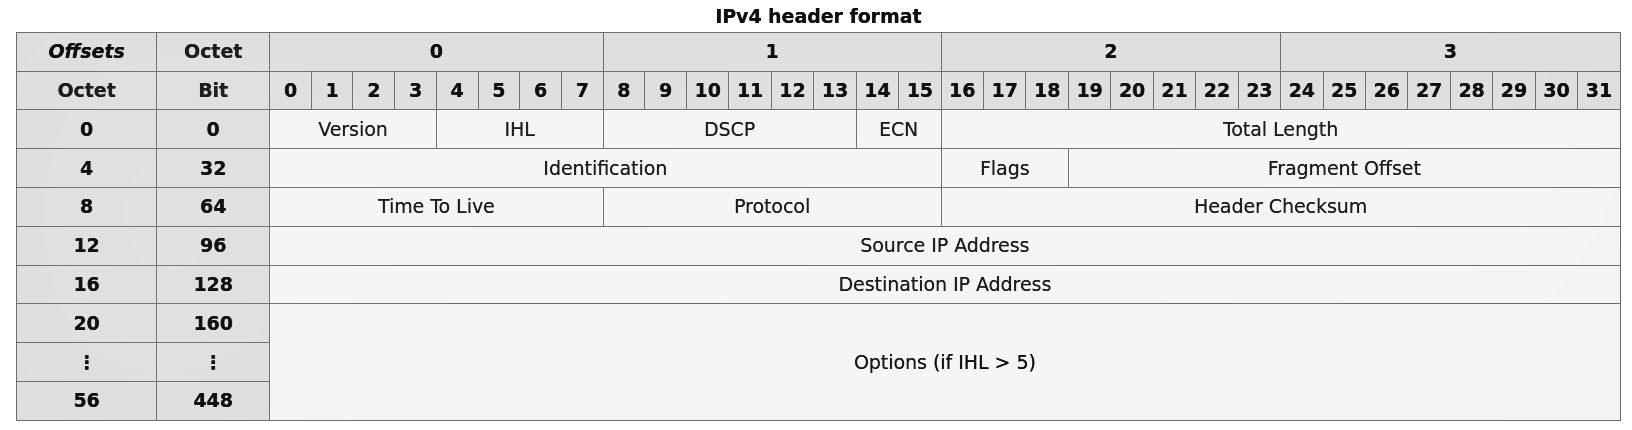
\includegraphics[ width=1.2\linewidth, height=\textheight, keepaspectratio]{./pics/tcp/ipHeader.png}
    \caption{Header of an IP packet. Source: Wikipedia.}
    \label{fig:ipHeader}
\end{figure}

Figure~\ref{fig:ipHeader} shows the structure of an IP packet. Essentially,
\begin{description}
    \item[Version, 4 bit] The first header field in an IP packet is the four-bit version field.
        For IPv4, this is always equal to $4$;
    \item[Internet Header Length (IHL), 4 bit] The IPv4 header is variable in size due to
        the optional 14th field (options). The IHL field contains the size of
        the IPv4 header, it has 4 bit that specify the number of 32-bit words
        in the header. The minimum value for this field is 5, which
        indicates a length of $5 \times 32 b = 160 b = 20 B$. As a 4-bit
        field, the maximum value is 15, this means that the maximum size of the
        IPv4 header is $15 \times 32 \mbox{ bit } = 480 \mbox{ bit } = 60 \mbox{ bytes }$.;
    \item[Differentiated Services Code Point (DSCP), 6 bit] Originally defined as the
        type of service (ToS), this field specifies differentiated services
        (DiffServ) per \texttt{RFC 2474}. Real-time data streaming makes use of the
        DSCP field. An example is Voice over IP (VoIP), which is used for
        interactive voice services;
    \item[Explicit Congestion Notification (ECN), 2 bit] This field is defined in RFC
        3168 and allows end-to-end notification of network congestion without
        dropping packets. ECN is an optional feature available when both
        endpoints support it and effective when also supported by the
        underlying network;
    \item[Total Length, 16 bit] This 16-bit field defines the entire packet size in
        bytes, including header and data. The minimum size is 20 bytes (header
        without data) and the maximum is $65535 B$. All hosts are required
        to be able to reassemble datagrams of size up to $576 B$, but most
        modern hosts handle much larger packets. Links may impose further
        restrictions on the packet size, in which case datagrams must be
        fragmented. Fragmentation in IPv4 is performed in either the sending
        host or in routers. Reassembly is performed at the receiving host;
    \item[Identification, 16 bit] This field is an identification field and is
        primarily used for uniquely identifying the group of fragments of a
        single IP datagram. Some experimental work has suggested using the ID
        field for other purposes, such as for adding packet-tracing information
        to help trace datagrams with spoofed source addresses, but RFC 6864
        now prohibit any such use;
    \item[Flags, 3 bit] A three-bit field follows and is used to control or
        identify fragments. They are (in order, from most significant to least
        significant):
        \begin{itemize}
            \item bit 0: Reserved; must be zero;
            \item bit 1: Don't Fragment (DF);
            \item bit 2: More Fragments (MF).
        \end{itemize}
        If the DF flag is set, and fragmentation is required to route the packet,
        then the packet is dropped. This can be used when sending packets to a host
        that does not have resources to perform reassembly of fragments. It can
        also be used for path MTU discovery, either automatically by the host IP
        software, or manually using diagnostic tools such as ping or traceroute.
        For unfragmented packets, the MF flag is cleared. For fragmented packets,
        all fragments except the last have the MF flag set. The last fragment has a
        non-zero Fragment Offset field, differentiating it from an unfragmented
        packet;
    \item[Fragment offset, 13 bit] This field specifies the offset of a particular
        fragment relative to the beginning of the original unfragmented IP
        datagram in units of eight-byte blocks. The first fragment has an
        offset of zero. The $13$ bit field allows a maximum offset of $(213 –
        1)\times 8 = 65528 B$, which, with the header length included $(65528 +
        20 = 65548 B)$, supports fragmentation of packets exceeding the maximum
        IP length of $65535 B$;
    \item[Time to live (TTL), 8 bit] An eight-bit time to live field limits a
        datagram's lifetime to prevent network failure in the event of a
        routing loop. It is specified in seconds, but time intervals less than
        1 second are rounded up to 1. In practice, the field is used as a hop
        count—when the datagram arrives at a router, the router decrements the
        TTL field by one. When the TTL field hits zero, the router discards the
        packet and typically sends an ICMP time exceeded message to the
        sender. The program traceroute sends messages with adjusted TTL values
        and uses these ICMP time exceeded messages to identify the routers
        traversed by packets from the source to the destination;
    \item[Protocol, 8 bit] This field defines the protocol used in the data portion of
        the IP datagram. IANA maintains a list of IP protocol numbers as
        directed by \texttt{RFC 790};
    \item[Header checksum, 16 bit] The 16-bit IPv4 header checksum field is used
        for error-checking of the header. When a packet arrives at a router,
        the router calculates the checksum of the header and compares it to the
        checksum field. If the values do not match, the router discards the
        packet. Errors in the data field must be handled by the encapsulated
        protocol. Both UDP and TCP have separate checksums that apply to their
        data. When a packet arrives at a router, the router decreases the TTL
        field in the header. Consequently, the router must calculate a new
        header checksum;
    \item[Source address, 32 bit] This field is the IPv4 address of the sender of the
        packet. Note that this address may be changed in transit by a network
        address translation device;
    \item[Destination address, 32 bit] This field is the IPv4 address of the receiver
        of the packet. As with the source address, this may be changed in
        transit by a network address translation device;
    \item[Options, up to 288 bit] Options are largely unused, and may be considered harmful by
        some router. This is the portion of the IP header that is variable in
        size.
\end{description}


\begin{figure}[h]
    \centering
    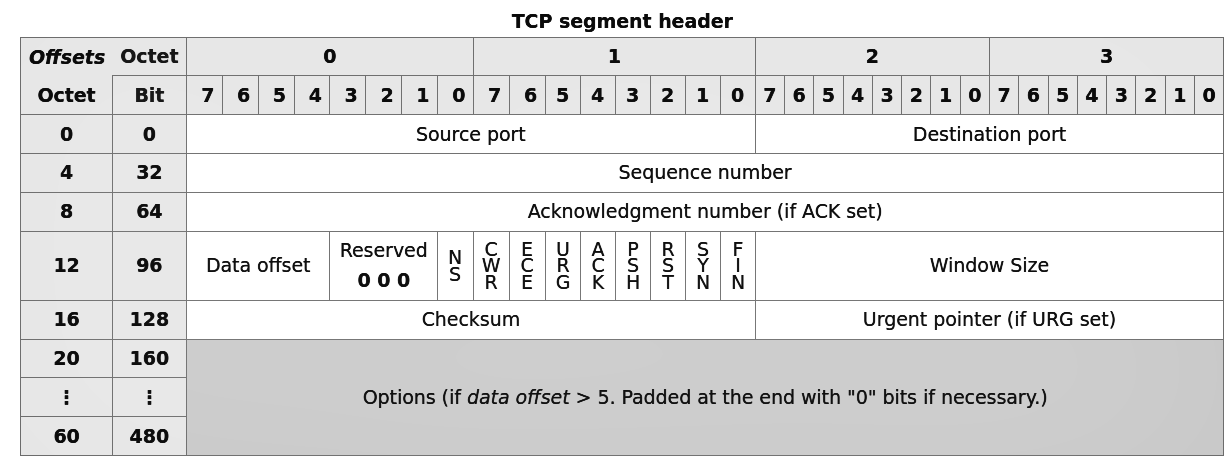
\includegraphics[ width=1.0\linewidth, height=\textheight, keepaspectratio]{./pics/tcp/tcpHeader.png}
    \caption{Header of a TCP segment.}
    \label{fig:tcpHeader}
\end{figure}

On the TCP header, instead, Figure~\ref{fig:tcpHeader} shows the header
structure,

\begin{description}
    \item[Source port, 16 bit] Identifies the sending port;
    \item[Destination port, 16 bit] Identifies the receiving port;
    \item[Sequence number, 32 bit] Will be covered later, its role is to keep
        track of the sequence of segments;
    \item[Acknowledgment number, 32 bit] Same as the above, but keeps track
        of the \emph{successfully delivered} packages;
    \item[Data offset, 4 bit] Specifies the size of the TCP header in 32-bit
        words. The minimum size header is 5 words and the maximum is 15 words
        thus giving the minimum size of 20 bytes and maximum of 60 bytes,
        allowing for up to 40 bytes of options in the header. This field gets
        its name from the fact that it is also the offset from the start of the
        TCP segment to the actual data;
    \item[Reserved, 3 bit] For future use and should be set to zero;
    \item[Flags, 9 bit] Contains $9$ flags, with some important ones:
        \begin{description}
            \item[URG] Indicates that the Urgent pointer field is significant;
            \item[ACK] Indicates that the Acknowledgement field is significant. All
                packets after the initial SYN packet sent by the client should have
                this flag set;
            \item[PSH] Push function. Asks to push the buffered data to the
                receiving application;
            \item[RST] Resets the connection;
            \item[SYN] \emph{Synchronize sequence numbers}. Only the first packet sent
                from each end should have this flag set. Some other flags and
                fields change meaning based on this flag, and some are only valid
                when it is set, and others when it is clear;
            \item[FIN] Last packet from sender.
        \end{description}
    \item[Window size, 16 bit] The size of the \emph{receiving window}. It is
        the number of window size units that the sender of this very segment is
        willing to receive. Useful in flow control;
    \item[Checksum, 16 bit] Checksum for error\--checking;
    \item[Urgent pointer, 16 bit] If the URG flag is set, then this 16-bit
        field is an offset from the sequence number indicating the last urgent
        data byte;
    \item[Options, variable 0–320 bit, in units of 32 bit] Various options.
\end{description}

\subsection{TCP Architecture}

\subsubsection{TCP bears an unpredictable and unrepeatable nature}

TCP carries many different implementations, depending mostly on OS of choice.
Several variants of its components have been written, with many of them largely
optional, or deprecated. As already mentioned, execution flow at application
level works independently and unpredictably with respect to the TCP-level flow:
when an application sends something, multiple TCP packages are exchanged;
how many and when they are sent is \emph{not predictable}.

TCP works by first copying data that should be sent in a buffer, and then send
them later.

The sequence of bytes is first copied to a buffer (sliding window) and the
\texttt{send()} function is, for example, invoked \--- the exact time in which a
segment is sent is \textbf{unpredictable}, \textbf{unrepeatable} and depends on
many things, over which the application has little to no control. This means
that application cannot \emph{deterministically predict} the exact time in
which the transmission will occur \--- instead, the TCP layer will deliver the
payload at a specific time determined by the protocol\footnote{However, also on
TCP layer there is a level of unpredictability. Many more effects can concur: for
instance, the Operating System may not be ready to send a segment, or may be
busy with other resources. These situation will cause delay in sending
information, even from the TCP layer's point of view.}.

On TCP, various \emph{events} can induce a transmission of data:

\begin{itemize}
    \item application invokes \texttt{send()} \--- in this case, the data in
        send's call argument will be inserted into the proper transmission
        buffer, and it will be transmitted somewhere in the (possibly
        immediate) future; 
    \item application invokes \texttt{receive()} \--- this way, we will see in
        detail that the TCP protocol will send a \emph{response} that
        \emph{acknowledges} the receipt of a segment, for the other party's
        sake;
    \item TCP layer \emph{receives a segment} \--- the same as above;
    \item a \emph{timeout} occurs \--- TCP layer will inform the other party of
        this;
\end{itemize}

Each of the above will trigger a transmission either immediately or
\emph{within a maximum predefined time} (in the case of a timeout, for
instance). When a TCP layer ``is touched'' from above or below, \textbf{it reacts
by transmitting a segment}. Transmission should occur \emph{even if there is no
useful data to transmit} (e.g. if the transmission buffer is empty) \-- in that
case, a segment will only carry the header, which has information useful to the
protocol itself. Basically, regardless of the presence of data in the
transmission buffer the TCP protocol will exchange vital protocol information.
Protocol information is, in fact, necessary to keep the connection alive and
well-performing.

Upon transmission, TCP may deliver a varying number of bytes, ranging from
empty up to a number of bytes \emph{larger than Maximum Segment Size} (536 in
Internet network, 1460 for same Ethernet network). Since huge payloads cannot
fit into a single segment with a predefined MSS, the TCP protocol
\emph{fragments} them before delivery, resulting in \emph{multiple segments
delivered in sequence}. TCP protocol will try its best to send as many segments
as possible, for efficiency's sake: it is not uncommon that $2$ or $3$ segments
are initially delivered before receiving the other party's response.

\begin{table}[ht]
\centering
\begin{tabular}{cc}
CPU Cycle & 0.3 ns \\
Main Memory Access (DRAM) & 120ns \\
SSD & 50--150 $\mu s$ \\
HHD & 10 ms \\
Internet, San Francisco to New York & 40ms
\end{tabular}
\caption{Some interesting metrics. Notice the order of magnitudes differences
between CPU cycles and network delays. This table highlights the fact that
bytes cannot be injected through the internetwork at full\--speed: suppose one
has a 100MB transmission buffer that is delivered across just 1ms \--
injected throughput would be $100 \cdot 10^6 \cdot 8 b/(10^{-3} s)$, which
yields an astonishing $8 \cdot 10^{11} b/s = 800 Gb/s$, unsustainable for most
of internetworks.}
\label{tab:SomeMetrics}
\end{table}
\bigskip

The TCP protocol starts with \emph{slowly sending segments, increasing the exchange
speed as the time goes on}. Acceleration mainly depends on the timing of
\emph{received} segments, by looking at the metrics of confirmation packets
from receiver. As the sender acknowledges that the receiver is able to keep up
with the increasing transmission speed, it raises up the delivery speed. Basically, TCP layer adapts its speed to $2$ determining factors,
\begin{itemize}
    \item the receiver's speed at processing packages;
    \item the internetwork's capability of deliver packages.
\end{itemize}

As we will see in following chapters, the first factor is handled by the
\textbf{Flow Control} algorithm, while the second one is kept under control by
the \textbf{Congestion Control} system.

\subsubsection{How an application asks for data to be transmitted}

The system call \texttt{send()} processes the data transmission through the
network. The \texttt{send} function passes a memory buffer contained in
application space (address, length), and copies bytes from transmission memory
buffer in application space to transmission memory buffer in TCP layer (called
\textbf{TX-buffer}).

\begin{lstlisting}
public void write(byte[] b)
	throws IOException
\end{lstlisting}

Send is first invoked by application level, whose execution flow is completely
independent from the TCP layer's one. Buffer at application layer is then
copied to the TCP transmission buffer, to be sent immediately or later. New
invokations of \texttt{send()} will copy data in TCP buffer \textbf{after} the
data that is already present.

Invoking \texttt{send()} \textbf{does not guarantee} any immediate
transmission: all it does is pushing application data into TX-buffer to be sent
in future. TCP will then \emph{independently} establish the proper moment and
way to transmit data present in transmission buffer.

Suppose now one has to send $N$ bytes with $K$ consecutive \texttt{send()}
invocations. How many segments will be exchanged? How many transmission events?

First and foremost, the number of segments will not depend on $K$, since no
matter how many times \texttt{send()} is invoked, the end result will be to simply
insert those $N$ bytes in the TX-buffer, because the sole effect of
\texttt{send()} is to insert the passed number of bytes into the TX-buffer,
triggering a transmission. As a first approximation, the number of transmitted
segments will roughly be $$\mbox{\#transmitted } = \frac{N}{MSS} + 1,$$ with
the last segment $+1$ smaller than the previous ones. Things, however, can go
wrong and be much more complex due to packet loss and retransmissions. Recall
that for all these reasons, the exact number is neither predictable nor
repeatable.

\subsubsection{Retrieving data from TCP}

Data retrieval occurs with another system call, \texttt{receive()}. System call
\texttt{re\-cei\-ve()} is quite similar to the \texttt{send()} call: both
receiver's TCP layer and Application layer execution flows act independently to
each other, and receiving buffer is not guaranteed to contain any data.

When data reaches the receiver, the data is copied into the receiving buffer
(\textbf{RX-buffer}). The receiving buffer stores all received bytes and is
flushed only when the application invokes \texttt{receive()}. The function
\texttt{receive()} copies (at least a portion of) the receiver buffer into the
application buffer by means of passing a buffer with known \emph{address} and
\emph{length}. Function \texttt{receive()} copies bytes without exceeding the
size of the buffer (\emph{length}) and it \textbf{returns} how many bytes have
been copied into the provided buffer. As argument, \texttt{receive()} also
takes the number of bytes to fetch from the TCP receiving buffer. Basically,
\texttt{receive()} needs to accept a buffer to which data should be copied, its
length (in C length information is \textbf{not} intrinsic to arrays) and the
expected number of bytes to be retrieved.

There are three possible outcomes for the \texttt{receive()} call:

\begin{itemize}
    \item the \emph{receive buffer is empty}: the application is suspended and
        the process is put to sleep until some data is available;
    \item \emph{more than \texttt{length} bytes are available}: a
        \texttt{length} number of bytes is fetched and delivered to the
        application as soon as possible. More \texttt{receive()} calls are
        needed to retrieve all data and empty the RX-buffer;
    \item \emph{less than \texttt{length} bytes are available}: all available
        bytes are copied as soon as possible, since they are less than the
        maximum deliverable value. The single \texttt{receive()} call will not
        yield all requested bytes, and more calls should be used.
\end{itemize}

Basically, each time a number of bytes is requested, TCP will provide \emph{up
to} that number of bytes. The application is held back only in the case when there
is no data available.

Now with an example: let a buffer have length equal to $800$ bytes. Suppose
\texttt{receive()} is invoked in the following scenarios,
\begin{enumerate}
    \item in the first scenario, there are $600$ bytes in the RX-buffer. Upon
        \texttt{re\-cei\-ve()} call, all $600$ bytes are delivered to the
        application. The RX-buffer is now empty;
    \item in the second scenario, there are $1000$ bytes in the RX-buffer. Upon
        \texttt{receive()} invocation, only $800$ of the $1000$ bytes are saved
        into the buffer \-- $200$ bytes will remain into the RX-buffer;
    \item in the third scenario, there is \emph{no data} in the TX-buffer.
        Application is suspended until there is data to retrieve. Suppose $500$
        bytes are collected in the RX-buffer \-- they will be immediately saved
        into the buffer provided by the application, and the application will
        retrieve them. RX-buffer is now emptied.
\end{enumerate}


\subsection{Sequence numbers}

IP protocol is \emph{unreliable} (packets can be lost, duplicated, or delivered
in different order from which they were sent). To overcome this huge
shortcoming, each data byte is implicitly identified by a $32$ bit
\textbf{sequence number}. A sequence number is a label for each transmitted and
received byte, so that both correct ordering and amount of data can be properly
determined. The association is \emph{implicit} \--- the sender applies a
sequence number to a segment, and the receiver uses that information to
reconstruct the original order of segments. This way, segments are
reconstructed even if they show up haphazardly, and the data can be assembled
as it originally was.

There are many variables involved in sequence numbers. \texttt{snd.User} is the
variable carrying the value of the next byte the \textbf{application} will
send. The variable \texttt{snd.Next} carries the value of the next byte that
the \textbf{TCP layer} will transmit \--- its value is contained in the TCP
header (initial byte of the sequence, of course). Basically, \texttt{snd.User}
refers to the next byte that will be filled by the invocation of
\texttt{send()}, while \texttt{snd.Next} is the next byte yet to transmit by
the TCP layer. The sequence number of application level must be computed from
other information. 

The variable \texttt{snd.Next} is carried in the TCP segment header, in
\emph{sequence number} space (16 bit).

In short,

\begin{itemize}
	\item \texttt{snd.Next} is the boundary between transmitted data and
		yet-to-transmit data;
	\item \texttt{snd.User} is the boundary between in TX-buffer data (data
        sent by application) and not-yet-associated bytes, the free space in
        the buffer.
\end{itemize}

Upon sending a segment, the \emph{sequence number} will be inferred from the
\texttt{snd.Next} variable, and will be the \emph{next byte the other endpoint
expects}.

\begin{figure}[b]
        \centering
        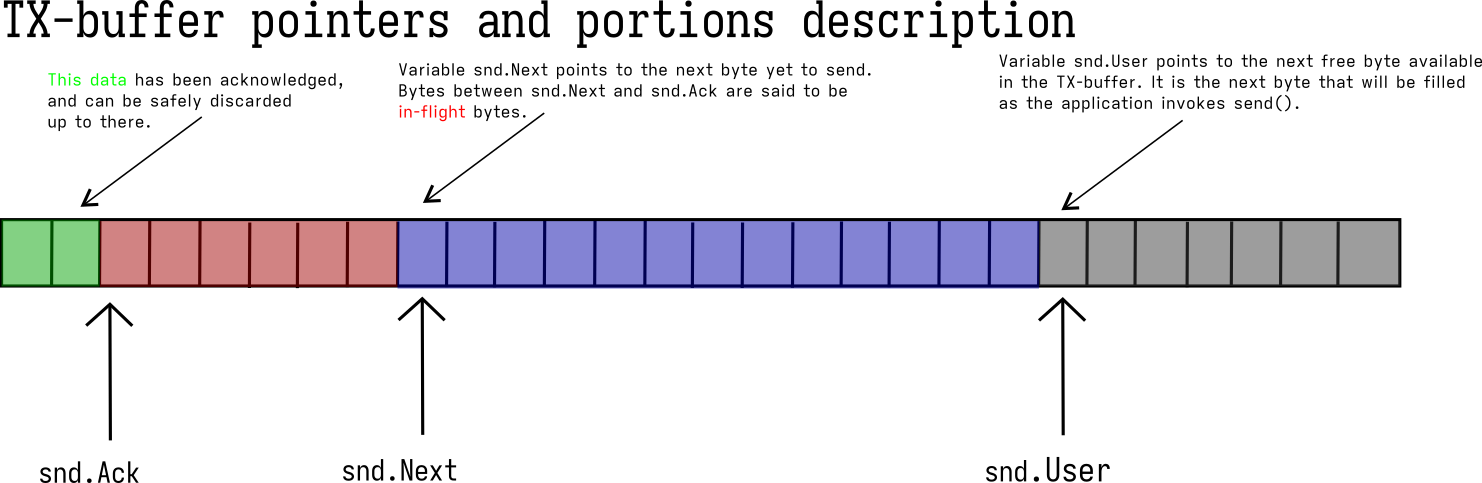
\includegraphics[ width=1.2\linewidth, height=\textheight, keepaspectratio]{./pics/tcp/TxBuffer.png}
	\caption{TX-Buffer and its flags \texttt{snd.Ack}, \texttt{snd.Next} and \texttt{snd.User}.}
        \label{fig:TxBuffer}
\end{figure}

From the receiver's point of view, the variable \texttt{rcv.Next} is the
boundary between content of RX-buffer and not-yet-received data (right boundary
of the data currently in buffer). The variable \texttt{rcv.Next} is similar to
the variable \texttt{rcv.Next} in the sense that it points at the next byte yet
to receive. Only packets having the \emph{expected sequence number} are collected
and brought into the buffer.

There is a special case where some segment carries new parts of information and
sequence numbers that are not collected, with a portion of them already
collected: in that case the incoming segment will still be collected, with
duplicated bytes thrown away. There may be two reasons for packet duplications:
either IP layer duplicates them, or the TCP sender retransmits them because it
thought they were lost. In order to be able to retransmit packets, TCP stores
all sent data in buffer until acknowledgement has been received, since they
could be retransmitted in the immediate future.

\begin{itemize}
    \item \texttt{rcv.Next} points at the next byte that is not yet being
        received;
    \item \texttt{rcv.User} points to the next byte to be received by the
        application. After \texttt{receive()} invokation by the application,
        all bytes that have been successfully delivered to the application can
        now be safely deleted.
\end{itemize}

\begin{figure}[b]
        \centering
        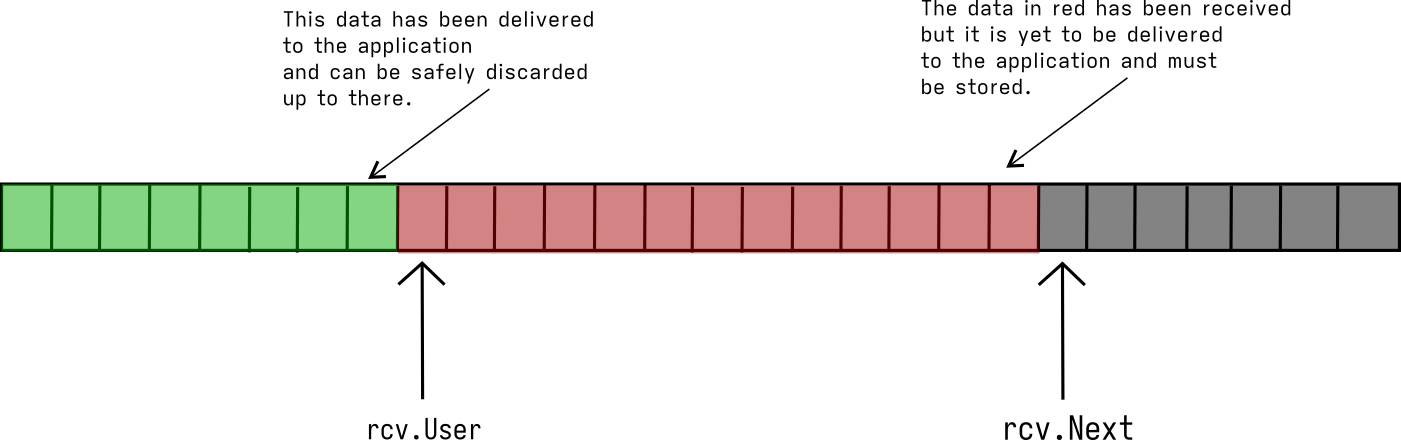
\includegraphics[ width=1.0\linewidth, height=\textheight, keepaspectratio]{./pics/tcp/RxBuffer.png}
    \caption{RX-buffer and its flags. Notice that RX-buffer only uses two flags
    instead of three (no ACK flag needed). Indeed, there is no need to keep
track of sent ACKs: they will be sent as soon as segments are acquired.}
        \label{fig:RxBuffer}
\end{figure}


Each TCP layer has \textbf{both} TX-buffer and RX-buffer. Sequence numbers in
the two directions are independent each other, and they will increase as much
as there is new data incoming from a direction.

Each and every segment is accepted only if it contains \emph{new} data: that
is, when the sequence number is the expected one \emph{or} when the segment
contains novel sequence numbers. 

Each segment also carries information on the \emph{length} of its payload. This
allows the receiver to efficiently reconstruct the segment, in order to compute
the ending sequence number, and not only the starting sequence number.

An important remark is that \textbf{sequence numbers are 32-bit integers}.
Therefore, the sequence numbers can only go from $0$ to $2^{32} - 1$, so there
may be \emph{wrap-arounds} in an overflow-like fashion. TCP should internally
handle these comparisons in a proper manner.

\subsection{Handling duplicates and loss}

IP is an unreliable protocol. This means that \emph{packets can be loss}.
Necessary mechanisms are two,

\begin{itemize}
    \item the \textbf{retransmission}, or when a segment is regarded to be
        sent again;
    \item the \textbf{acknowledgement}, which is a kind of \emph{notification
            of receipt}, that is sent by the receiver in order to make the
            other party sure that it has received and collected the data sent
            to it.
\end{itemize}

\emph{Acknowledgements} are a mechanism that assures receipt of a message by
means of \emph{notifications}. Every header of a segment contains the sequence
number of \texttt{snd.Next}. Every segment also \emph{carries an information
regarding the bytes that are received}: the \textbf{acknowledgement number},
which tracks the state of the RX-buffer by following the pointer
\texttt{rcv.Next}. This way, having both sequence number and acknowledgement
number, one can successfully track the state of a TCP connection. Upon sending
a TCP segment, both sequence number and acknowledgement number are delivered,
so that the receiver can reconstruct the state of the sender RX-buffer.

Basically, sequence number tracks the bytes a party \emph{has sent}, while
acknowledgement number tracks the bytes a party \emph{has successfully
received}. Both informations must be exchanged at every delivered segment.

A fifth variable is thus needed: \texttt{snd.Ack}, which \emph{points to the
byte in TX-buffer before which any transmitted byte had been acknowledged}.
This variable is only increased upon receiving data (for instance, upon
receiving a sequence with a greater ACK number from the sender). Since it has
been safely collected, all data before \texttt{snd.Ack} pointer can be
forgotten. 

Acknowledgements mechanism is crucial to a TCP connection, in order to
provide \textbf{reliability} to a connection. Therefore, transmission of
acknowledgements is always necessary even if TX-buffer is empty. In that case, no
payload will be transmitted, and only protocol information is sent (increasing
acknowledgement number).

An important note is that \texttt{snd.Ack} is only updated when the received
sequence number \texttt{segment.ack} is \emph{greater} than the value in
\texttt{snd.Ack} \-- that is, when new data are correctly received.

For this reason one can say that the sequence number tracks \texttt{snd.Next},
while the acknowledgement number tracks \texttt{rcv.Next}. However, the
sequence number will be at the value of the \emph{first} sent byte, that is the
first byte the receiver is expecting.

For instance, suppose the receiver has successfully received $130$ bytes from a
sender: its \texttt{rcv.Next} points to the $130$th index in the RX-buffer,
corresponding to the $131$th byte. In order to inform the sender, all the new
incoming segments from the receiver will carry $130$ as sequence number (it
points to the $131$st element). Upon receiving such packets, the sender will
successfully interpret the sequence number, and set the \texttt{snd.Ack}
variable to $130$: all the data prior to index $130$ can be safely discarded.

Data bytes between pointers \texttt{snd.Ack} and \texttt{snd.Next} is said to
be \textbf{in flight} data. These bytes have been transmitted but not yet
acknowledged, and are potentially eligible for retransmission.

The reason why acknowledgements are important is pretty straightforward: without
acknowledgements, there would be \textbf{no way for the sender to tell whether
sent data has been received or not}. This means that even though the receiver
has no data, acknowledgements are still required and should be properly sent.

In the end, acknowledgements are a crucial component of TCP, without them it
wouldn't be possible to provide either a reliable or a predictable connection,
with no chance of keeping track of actually and successfully delivered
information.


\subsection{Delayed Acknowledgement}

\emph{Delayed Acknowledgement} is a notorious TCP algorithm. Its core idea is
not to answer immediately with an acknowledgement, but to await some arbitrary
time interval $T$ that depends on the operating system. The algorithm is pretty
straightforward:

\begin{quote}
Upon receiving a segment, if delayed-ack timer $T$ has previously been set,
\emph{transmit immediately}. Else, set the delayed-ack timer $T$ to a specific
value.
\end{quote}

When receiving a packet, simply set a timer, and send the response segment
after timer expires. However, if you receive yet another segment before the
timer expires, then send immediately the response.

Delayed-ack timer value depends on the operating system:

\begin{itemize}
    \item RFC suggests $T = 500ms$;
    \item Windows has $T = 200ms$;
    \item Linux in general has $T = 40ms$;
    \item RHEL sets $T = 4ms$.
\end{itemize}

The reasoning is as follows: if there is not much data to transmit, it will be
likely that the timer $T$ will expire. Expiring timer means sending a packet
with the proper acknowledgement number \-- a strategy that guarantees that the
connection stays open and remains fresh. If the other part is sending a lot of
data, the contrary will be more likely to occur, breaking the awaiting. In
order to help the other part, acknowledges will be delivered as soon as a
\emph{second segment} is received. 

The core idea is to both help the other end and
minimize the number of segments to be sent: this is done by preventing to
respond with a segment whose sole purpose is to inform of acknowledged data
\emph{at each segment received}, while still answering with ACK information
even though there is little to no data received. In fact, a delay time $T$
assured to save sending some segments, a feature that historically was of a
crucial importance.

\subsection{Retransmissions}

The connection state includes three more actors, related to
\emph{retransmission}:

\begin{itemize}
    \item a \textbf{retransmission timer}, which counts the time interval until
        which the retransmission is held back;
	\item a variable that describes the \emph{current duration of the retransmission
        timer interval}, the \textbf{RTO (Retransmission Time-Out)};
    \item a \textbf{retransmission counter}, that counts how many
        retransmissions for a segment have been performed.
\end{itemize}

The \textbf{retransmission algorithm} is as follows:

\begin{quote}
    Upon transmitting segment S, \emph{if timer is not already set}, then the
    counter is cleared and set to $0$, with the timer set to the RTO value.
    At the beginning, then, a new counter is spawned and the timer is set to
    a value which is the RTO value.

    When an ACK is received, \texttt{snd.Ack} is updated to the maximum value
    between \texttt{snd.Ack} and \texttt{segment.Ack}. If \texttt{snd.Ack ==
    snd.Next}, the timer is switched off: the sent data has been received by
    the other party correctly and as expected.

    There may be occasions in which the timer expires, though.
    When timer expires, the \emph{counter is incremented} and if the counter
    has not yet reached a \texttt{MAX\_COUNT} value, the segment is
    retransmitted. However, this time the timer value is set to RTO but
    \texttt{RTO = 2 * RTO}, which is the double of the original value.
    \emph{Only in-flight data should be retransmitted} (and all of it after
    timer expires). Basically, data for which we are sure that it has been
    received should not be retransmitted in case the timer expires, and the
    sender should only focus on retransmitting not-yet-acknowledged data. At
    each retransmission, the RTO is doubled, and the retransmission counter is
    increased.

    When counter reached \texttt{MAX\_COUNT} value, an excessive number of
    retransmissions has been attempted, and connection is closed.

    Upon receiving an ACK for \textbf{all} the in-flight data, switch the timer
    off (that is, when \texttt{snd.Ack == snd.Next}).

    A particular condition is when an ACK arrives \emph{for only a portion} of
    the data that has been sent. In that case, the timer resets (the receiver
    has responded) to the RTO value, \emph{as if those still not-ACKed had been
    sent now}, and the sender awaits ACK for missing segments. This basically
    occurs when a partial ACK comes, and prevents unnecessary retransmissions.
\end{quote}

Exact timings of retransmissions are hard to predict. A sender is completely
blind if it does not receive any ACK: should it send again in-flight segments,
or should it wait a little bit more? In practice, how long should the timer be
set? Basically, a rule of thumb is that it should be ``slightly larger'' than
Round\---Trip Time. In order to do so, since RTT largely varies depending on
connections, time, and many other conditions, RTO is \textbf{dinamically updated}
by algorithms such as \emph{Jacobson algorithm}.

Regarding the maximum number of retransmissions, value of \texttt{MAX\_COUNT}
largely depends on the operating system. For instance, Windows closes
connection after $5$ failed attempts, Linux after $15$. It is simple to realise
that there may be a lot of unnecessary retransmissions: the timer can, for
instance, run out too soon for the acknowledgement to reach the sender.
Unnecessary retransmissions are a waste of resources, and definitely a
fundamental problem. The reason could be one of those:

\begin{itemize}
    \item segments are \emph{lost}, retransmissions are necessary;
    \item there could be segments \emph{whose ACKs are lost};
    \item RTO was set to a \emph{too small value}.
\end{itemize}

Thus, RTO should be set to an appropriate value, since a too short value leads
to high overhead and possibly many unnecessary retransmissions, while a too
long value results in high latency and possibly a slow or non-responsive
connection. RTO value is basically a \emph{trade-off} between exhibiting few
retransmissions and having a fast and responsive connection. RTO should be set
\textbf{dinamically}: it should be slightly greater than the \emph{RTT}
(Round-Trip-Time), an idea from Jacobson algorithm. This is of a crucial
importance for TCP to work. Initial RTO value is heuristical, and varies from
one OS to another. Linux and Window start from same value, macOS use a
different value, and so on.


\subsection{Multiple default gateways}

More default gateways could be added to a single node. Reasons to add more than
one default gateway all boil down to \emph{failure avoidance}. To know whether a
gateway has stopped working, a heuristic TCP algorithm tries to detect a
gateway failure:

\begin{quote}
    If the number of retransmissions is greater than \texttt{MAX\_COUNT}
    divided by 2, the \emph{connection} changes its default gateway (if
    possible). Moreover, if the number of connections that changed default
    gateway is greater than the number of open connections divided by 4, the
    \emph{IP layer} changes the default gateway as well. This last feature
    speeds up reconfiguration of early connections that still have to make some
    retransmission attemps.
\end{quote}

Basically, each connection can autonomously choose its own gateway, but the IP
layer is able to \textbf{force} any \--- new or already present \--- connection
to use a different default gateway. A connection that exceeds the total number
of retransmissions will change default gateway, and if $4$ or more connections'
default gateway switches are detected the IP layer will switch to a different
default gateway as well, forcing all newly created TCP connections to switch to
the new gateway.


\begin{figure}[h]
    \centering
    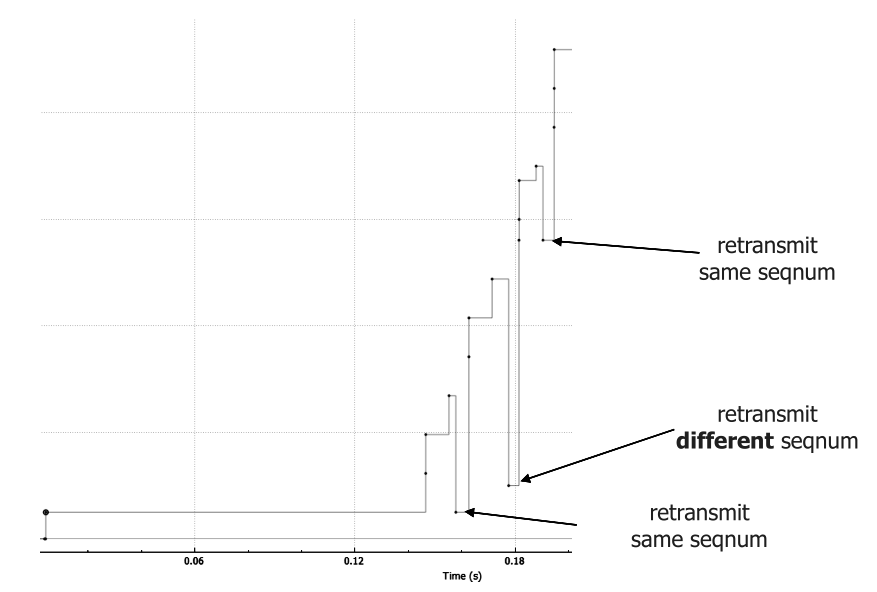
\includegraphics[ width=1.0\linewidth, height=\textheight, keepaspectratio]{./pics/tcp/timeSequenceTCP.png}
    \caption{Time plot of sequence numbers. Dots correspond to sent segments. Some retransmissions occur.}
    \label{fig:timeSequence}
\end{figure}

\subsection{Selective Acknowledgements}

Suppose that 4 segments are sent, and the second one has been lost: in this
case, the receiver got all segments except the second one, but it has
no way to inform the sender to retransmit only the second segment. Sending
ACK for only the first segment would result in unnecessary retransmission of
segments 3 and 4, which were instead correctly received. 

For this reason, the receive buffer could end up having some \textbf{gaps},
missing bytes that are supposed to be received. The solutions are
\textbf{Selective Acknowledgements} (SACK), a special kind of acknowledgements
that carry both \emph{left and right sequence number edges} of each
out-of-order \textbf{block} in RX-buffer, this way correctly informing the
other party of a \emph{specific} missing portion of the data, avoiding
unnecessary retransmissions. Selective Acknowledgements can selectively mark
which bytes should be transferred again, and only those.

SACK protocol must be \emph{supported by both members} of a connection in order
to be useful. The protocol is very convenient, since many segments can be lost
when a sender tries to deliver dozens of segments at once. This way, TCP can
achieve \emph{efficient handling} of the connection, minimizing the number of
unnecessary retransmissions.

In SACK\--supporting segments, a \texttt{TCP Option} field exist, in which both
\texttt{left edge} and \texttt{right edge} are inserted, and they allow for
correct data reconstruction after it has been lost, only for that portion
delimited by the two edges.

Of course, out-of-order segments could still lead to gaps in RX-buffer, causing
an unnecessary retransmission. In this case, unnecessary retransmissions are
unavoidable when an out-of-order segment reaches the receiver too late, after a
long time interval, since the receiver will send a SACK informing the sender of
the missing segment, while the very same segment arrives late. However, no
matter what, SACK is always convenient, since it reduces a lot the burden to
the sender for only missing segments are to be sent.

To optimize out-of-order gaps, \textbf{Fast retransmit} algorithm should be
adopted (not part of this course).

\subsection{Operating System TCP interrupts and the real TCP execution flow}

Upon packet arrival, a \emph{system interrupt} is sent. 

An operating system executes many concurrent activities: application process, other networking processes, manages other system interrupts, and so on.

When a system interrupt is cast, the operating system will try its best to fetch data from the network physical device.

From the TCP point of view, after data comes from the operating system, it will
analyze the packet to sort it by \emph{looking at the connection table}, and
then will \textbf{push in the input queue} the relative packet. The input
queue holds a certain amount of segments, stored in the order given by sequence
number.

When the TCP protocol decides it's time to process all segments in queue, it
deeply analyzes them, picks their payload, grabs their header information, and
processes all of them. After processing all segments in input queue, the buffer
is emptied.

Basically, TCP can never \textbf{immediately} process a segment upon arrival.
What it can do best, is to await some time, receive an amount of segments
depending on the operating system's load at that moment and many other factors,
and then process them altogether. Since many of them are processed at the same
time, only a single acknowledgement will be sent back to the sender.

Since there are \emph{many} different sources of randomness, let alone things
that are completely out of TCP's control (just think of connection's quality,
operating system's load, the other's end capabilities, packet loss,
send\---receive invocations), there is \textbf{no} single correct way for TCP
protocol to exchange a given amount of data with another party.

\section{Flow and Congestion Control}

To behave optimally, TCP needs to establish the correct amount of data that
should be exchanged in an interval of time.

Whenever TCP decides to transmit, there are three possible scenarios: 
\begin{enumerate}
    \item an empty segment is sent when there is no payload \-- that is the
        case, for instance, of acknowledgements or when timer expires;
    \item it transmits a single segment if payload data is smaller than MSS \--
        that is for few data;
    \item it transmits multiple segments if payload size exceeds MSS \-- that's
        the case for huge payloads.
\end{enumerate}

However, not all connections are equally good, and not all endpoints are fast
enough to cope with a sender's speed. A sender should not send more segments
than how many can be managed by the receiver \--- \emph{how many} is an upper
limit that should be dynamically changed.

The overall idea is the following one: TCP \textbf{starts slowly}, then
\emph{increases its transfer speed} according to the rate in which
acknowledgements are received. Since the interaction is bidirectional and
quite complicated, TCP implementation at sender's side tries to adapt to
both connection properties and receiver's side properties. 

As a general rule, the number of in-flight bytes is \emph{always lower than an
upper bound that is dynamically updated}, with an upper bound that is chosen
according to proper criteria. This means that TCP can automatically
\emph{adapt} to the peculiar characteristics of the connection and receiver's
speed.

In order to adapt the two different aspects of a TCP connection \-- the
\emph{connection quality} and the \emph{receiver's speed} \-- two bounds should
be adopted: the \textbf{Flow Control} and the \textbf{Congestion Control}. The
TCP layer will always send less data than the minimum between the two upper
bounds. 

The first algorithm constructs a bound in such a way that the capacity of the
receiver is always respected. Let an extremely fast computer send data faster
than a receiving, slow, computer. Slower computer has not enough speed to
collect all data that has been sent \--- the flow control algorithm lets the
sender speed adapt to the receiver speed by means of a \emph{send window}. 

The second algorithm, the congestion control, constructs a state variable
called \emph{congestion window}, whose goal is to \emph{model the maximum current
throughput of the network}. 

The number of in-flight bytes \emph{must be slower than both send window and
congestion window multiplied by MSS}, so that $$\mbox{in-flight} \leq
\min(\mbox{sndWin}, \mbox{congWin} \cdot \mbox{MSS}).$$ 

The mental model should be the following one: if the transmission buffer is
full of data, a number of in-flight bytes equal to the minumum of both
quantities should be sent, otherwise just send \texttt{snd.User - snd.Ack}
bytes (those still to send).

\subsection{Flow control}

Buffers cannot increase indefinitely: boundaries must be set in order to assure
system stability. In Linux kernel, buffer sizes are set upon compilation and are
then fixed; different operating systems may show other behaviors. In case data
cannot be pushed into the TX-buffer anymore because it is full, application
should be suspended. When the RX-buffer is full, packets have to be discarded
since they cannot be collected. Flow control will act to prevent this situation
by letting the sender know how much free space is available to the RX-buffer. 

The goal of flow control is to keep a fast transmitter from overrunning a
slower receiver.

Since application sends data much faster than ACK arrive, the TX-buffer could
end up being filled up by incoming segments. Suppose at receiver's side the
application invokes \texttt{receive()} much slower than incoming packages
speed. This way, the RX-buffer could fill up as well. To solve this issues, as
application invokes \texttt{send()} when TX-buffer is full, it is
put to sleep (blocked) until TCP gets proper ACK and advances \texttt{snd.Ack}
(when it has more free space).

TCP sender keeps track of free space in other end's RX-buffer by looking at a
variable in header (WindowSize) that informs it of how much free space is
available, so that it can actually predict how much free space there is. When
it guesses that receiver's RX-buffer could have no space left, it stops
transmission and suspends the application. If the maximum window corresponds to
the size of a single segment, the protocol is called \textbf{stop-and-wait}
(that is \-- send a single segment, then wait for ACK). Larger windows enable
pipelining of multiple segments in a row, allowing far more efficient usage of
the connection.

Flow control algorithm adopts the concept of \textbf{sliding window}. Each
segment header has a \texttt{WindowSize} field in the header that contains
\emph{how many free bytes are in the RX-buffer}. From sender's point of view,
\texttt{snd.winSize} contains the \emph{number of free bytes in RX-buffer of
the other side}.

The value is initially set to the receiver's entire buffer size, and it is
updated dynamically upon sending a segment. If a segment \texttt{S} carries
\texttt{S.Ack} that is greater or equal to \texttt{snd.Ack}, then the variable
\texttt{snd.winSize} is updated and set to \emph{S.windowSize}. The
\texttt{snd.WinSize} value ranges from $0$ to the buffer size at the receiver's
end.

Ultimately, the number of in-flight bytes must never exceed the number of bytes
in \texttt{snd.winSize} that are available in the RX-buffer. This means that
\texttt{snd.Next - snd.Ack} should \textbf{never} be greater than
\texttt{snd.\-WinSize}.

The end goal of TCP is to reach a number of in-flight bytes that is as close as
possible to the \texttt{snd.winSize} number of bytes, in order to optimize the
connection efficiently.

\begin{figure}[b]
    \centering
    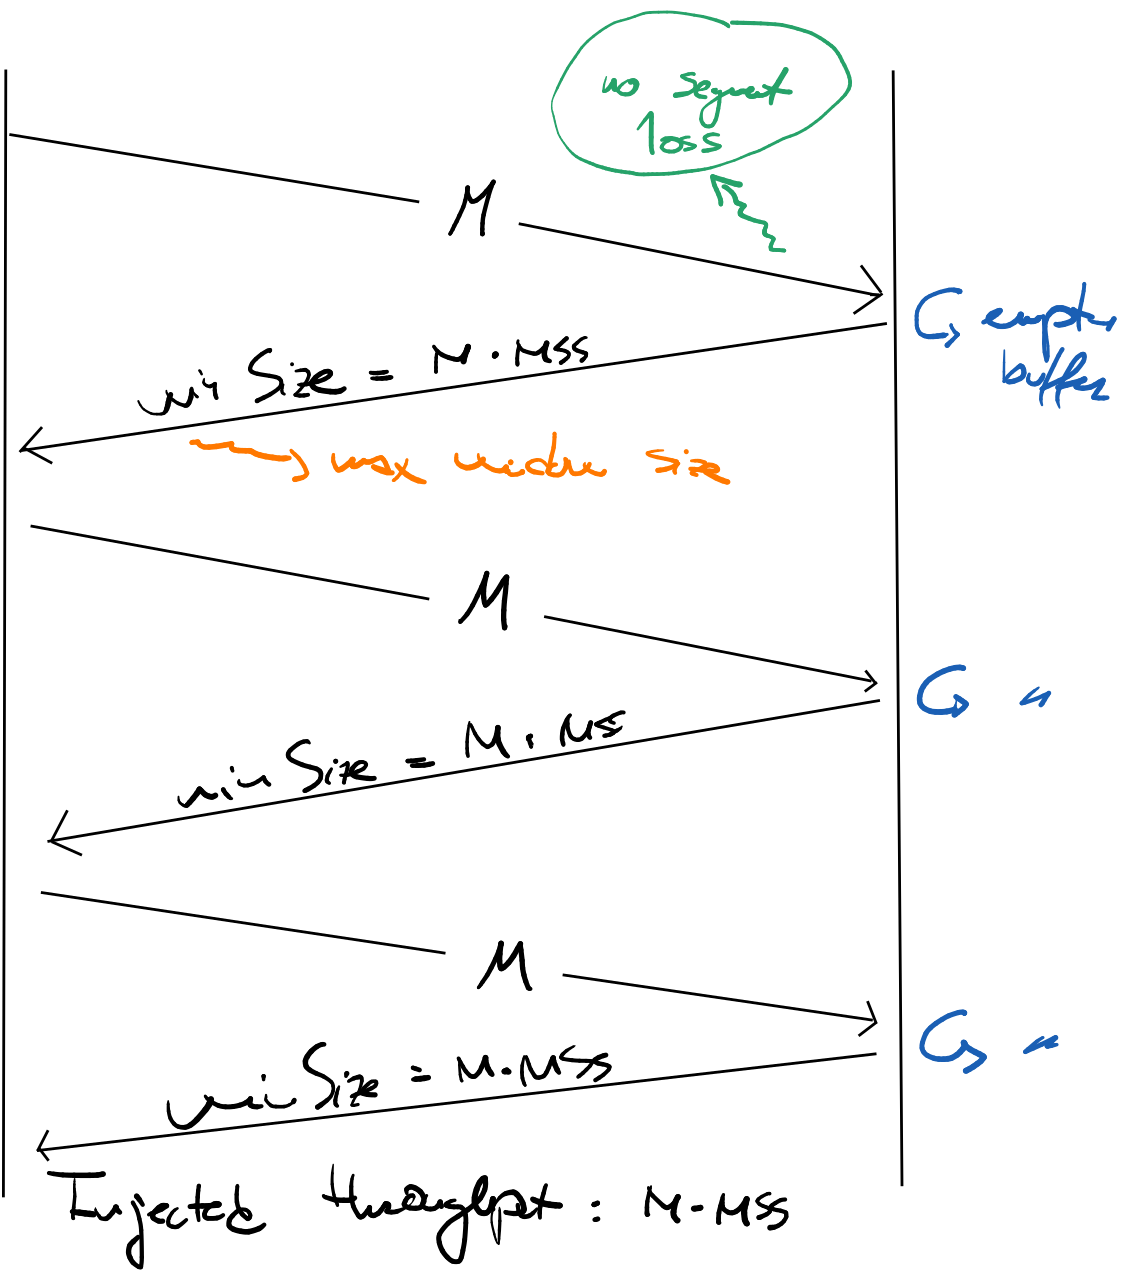
\includegraphics[ width=1.0\linewidth, height=\textheight, keepaspectratio]{./pics/tcp/idealThroughput.png}
    \caption{Ideal throughput condition, in which the injected throughput is
    equal to M $\cdot$ MSS at each time $T$. In scheme, every timing is
considered constant, and the total time $T$ is the sum of the time in which all
the segments arrive at the receiver's end, the receiver's processing time and
the acknowledgement's time to arrive at the original sender's side.}
    \label{fig:idealThroughput}
\end{figure}

\clearpage


\subsection{Performance estimation}

From flow control, let's determine the maximum T-IN-TCP (input throughput) that can be obtained.
TCP is injecting some throughput into the network, and the amount of it is
controlled by the flow control algorithm. 

Suppose the receiver has a window size of $M \cdot MSS$, and the application
requesting data invokes \texttt{receive()} on a large buffer, such that the
buffer is emptied as soon as there is new data.

The best case one can get by flow control is $M \cdot MSS$ every RTT \--- this is
the case where the receiver's application empties the RX-buffer the moment the
segments arrive. Suppose in fact $M \cdot MSS$ bytes are sent at each round,
and no packet loss occurs: in that case, the receiver would immediately and
successfully grab all segments, sending the corresponding acknowledgment
answer.

In the case the application empties \emph{half} the buffer at periodic
intervals, the throughput would be the half as well, $M/2 * MSS$ every RTT.
After the first round, only half of the segments would be sent, since the
window size is indeed the half of the total one. 

If the entire buffer is emptied at once, but with a delay, or not aligned with
the receipt of segments, the throughput would be $M * MSS$ every RTT + $\Delta$
(more time than plain RTT). Combining all cases, one could get less than $M *
MSS$ data every \emph{longer} than RTT, depending on the parameters and the
circumstances of the network.

For the best case, it's important to recall that some important assumptions
have been made:
\begin{itemize}
    \item all intervals have same time duration $T$, as described in
        Figure~\ref{fig:idealThroughput};
    \item all the segments arrive together, or at least not after a time which
        is irrelevant or already counted in $T$.;
    \item acknowledgement arrives immediately, and not after a huge delay;
    \item receiver is perfect in managing segments, and provides an
        acknowledgment segment for the full data.
\end{itemize}

In every case, a greater RX-buffer will result in higher throughput, since
there is a proportionality between throughput and buffer size. Viceversa,
greater RTT will result in less throughput \--- LANs will have greater
throughput than WANs since they possess a lesser Round\---Trip Time. However,
in this formula the \emph{quality} of the network is not taken in account:
segments can be loss, especially when too many of them are injected through the
internet. For this reason, this much-optimistic model cannot be applied in
cases where the throughput is high (read \--- when RX-buffer is insanely huge).
Every time a retransmission is needed, \emph{detection and recovery} takes
place, and throughput becomes much smaller than the ideal case. This
phenomenon is much heavier as the RTT increases, since retransmissions are
harder to assess; Moreover, it is far from being predictable.

Another thing to consider is \emph{maximum network speed}. Injected throughput could
be \emph{even greater} than maximum network speed, in that case many segments
would be loss, resulting in a sub-optimal efficiency\footnote{This is solved by
Congestion control mechanism.}.

\subsubsection{Establishing size of RX-buffer}

Size of RX-buffer should have the following characteristic: the size should be
\emph{a multiple of MSS} \--- this is done to avoid leaving unused space at the
end of the buffer, since in the lucky case exactly a multiple of MSS will be
delivered. Non\--multiple sizes would make no sense.

However, the RX-buffer size is a \emph{trade-off} between greater ideal
throughput and lower throughput due to excessive retransmissions, and should be
chosen accordingly. Unexpectedly, $64KB$ are chosen; the value is OS-dependent.
The size is managed as if it were a multiple of MSS \--- when almost full,
pretend it is full and ignore last portion of buffer.

\begin{table}[ht]
\centering
\begin{tabular}{ccc}
    Flow control & Ethernet & Internet \\
    MSS  & $1460B$ & $536B$ \\
    RX-buffer & $64KB$ & $64KB$ \\
    number of segments in-flight & $44$ & $122$
\end{tabular}
\caption{Quantities involved in flow control, on Ethernet and Internet.}\label{tab:FlowControlQuantities}
\end{table}
\bigskip

\subsection{Sustainable throughput}

A sustainable throughput is indeed \textbf{not infinite}. After a certain injected
throughput \texttt{T\_MAX}, the network bottlenecks and starts losing segments, exhibiting a
behavior that will lead to less performance. Thus, an optimal throughput should
be determined by and largely depends on \emph{connection quality}. Injected
segments are delivered at same speed only if the injected throughput is lower
than the maximum possible throughput, that is \texttt{T\_MAX}.

\begin{figure}[b]
    \centering
    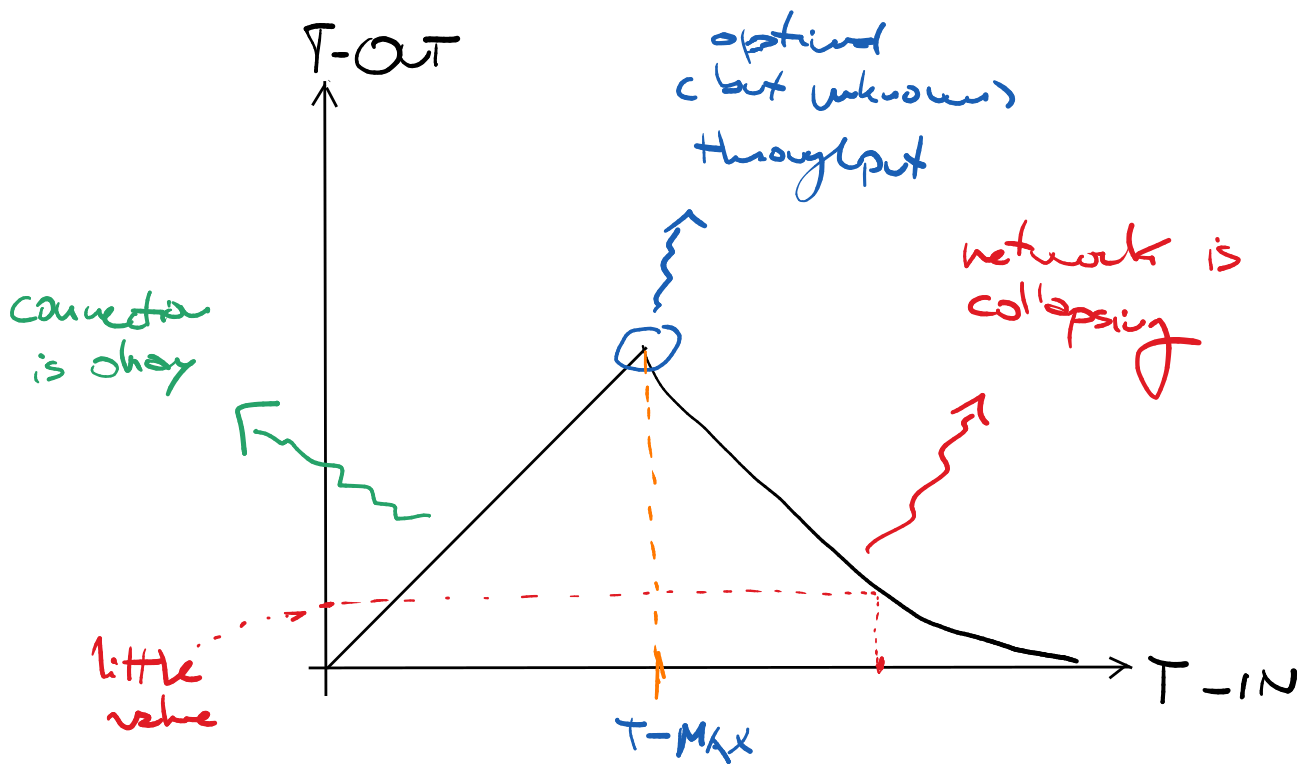
\includegraphics[ width=0.6\linewidth, height=\textheight, keepaspectratio]{./pics/tcp/networkCollapse.png}
    \caption{Network collapse after injecting a too-high throughput. Notice
        how injecting an even greater throughput will result in a \emph{lower}
        throughput.}
    \label{fig:networkCollapse}
\end{figure}


An excessive throughput \textbf{will} result in the following consequences:
\begin{itemize}
    \item packets exit \textbf{slower} than they entered;
    \item network's max sustainable throughput \texttt{T\_MAX} will
        \emph{collapse} \--- this fenomenon is called \textbf{network
        congestion};
    \item network \textbf{will need some time to remove its congestion},
        with even worse behavior in the case the unsustainable throughput is
        maintained for a longer time.
\end{itemize}

Intuitively, a network collapse happens because networks possess different
maximum speeds, a quality that cannot be appreciated by TCP, let alone for
networks \emph{different} than the one in which the device is sending data.

It is then up to the TCP layer to detect issues during path, and slow down
segments injection. Routers commonly have a mechanism for packet queuing, which
can be filled up, resulting in packet discarding. Such discarded packets will
need a retransmission, leading in even lower performance. New injected segments
and packets will increase the time for which the queue is dissolved.

\subsection{Congestion control}

\textbf{Congestion Control} algorithm takes into account the quality of the
network, allowing the sender to adapt to it instead of making it collapse.

Suppose the bound of flow control is so large that congestion control is
predominant (which means snd.congWin*MSS < snd.WinSize). A congestion control algorithm
could try do infer the maximum throughput by looking at the RTT and calculating
MSS/RTT < T\_MAX. However, this is unfeasible, since it requires too much
rounds and tentatives to be inferred.

A second issue is that the quantity T\_MAX \emph{varies during time}:
it depends on nominal throughput of networks and routers, and on
\textbf{competition} of different injected throughputs in the network.
Basically, the competition in the network is \emph{unpredictable} and
\emph{time-varying}, allowing no fixed\--value algorithm to work.

\subsubsection{Actual algorithm}

Congestion control algorithm has some important components,
\begin{enumerate}
    \item the \emph{slow start};
    \item the \emph{congestion avoidance};
    \item the \emph{fast retransmit};
    \item the \emph{fast recovery};
\end{enumerate}

each one with several variants and many parameters to be properly set. We will
see \emph{Tahoe} algorithm, but the most used one is the \emph{Reno}
algorithm.

The core idea of the TCP Congestion Control is to increase the so called
\textbf{congestion window}, a window size\--tracking variable, every time an
acknowledgement is received, while decreasing it a lot after a retransmission
timeout had expired, starting again from a lower speed. 

Initially, the
congestion window is set to a very low value: that is called \emph{the slow
start algorithm}. The slow start algorithm takes place if the congestion window
value is below a certain threshold, called \emph{SlowStartThreshold}; under the
slow start algorithm, the size of the congestion window increases very, very
quickly. After the congestion window size is above the threshold, the
\emph{congestion control algorithm} takes place, and makes the window increase
very slowly.

\begin{enumerate}
    \item The state variable \emph{CongestionWindow(t)} keeps track of a
        `virtual window' that is the actual quantity of data that can be
        injected through the network, and is initially set to a very small
        value (\emph{slow start principle}). Its value will increase whenever
        Acknowledgements are received in time \--- the network is assumed to be
        not congested. Upon retransmission (timeout expiration) the state
        variable is decreased a lot, and the network is assumed to be
        congested. 

    \item Another state variable, called \emph{SlowStartThreshold}, is
        a threshold under which \emph{CongestionWindow(t)} increases very fast,
        while above it the same state variable increases with a slower rate.
        Initial values of \emph{snd.congWin} and \emph{snd.ssThresh} are,
        respectively, $3$ MSS and $64KB$.

    \item Whenever an acknowledgement is received in time, the congestion
        window is increased. If the congestion window is lower than the
        threshold, increase fast with \textbf{slow start algorithm}; otherwise,
        increase slowly with \textbf{congestion avoidance} algorithm. The first
        will cause a fast growth in size of the window, the latter will instead
        produce a slower growth.

    \item Upon retransmission (timeout expiration), the congestion window is
        reset to MSS. Differently, the threshold is set to the maximum value between $2$
        MSS and \texttt{(snd.Next - snd.Ack)/2} \--- that is, the maximum value
        between the double of MSS and the half of the currently in-flight bytes. The
        assumption upon retransmission is that the network is congested: this
        behavior is inefficient in the case the network is not congested. Since
        \emph{many} concurrent causes may determine a packet loss \--- for
        instance, small RTO, network loss (e.g. WiFi) \--- one can end up with
        a congestion control algorithm forcing a slower pace of the network
        even though there is no actual congestion.

    \item The congestion window is increased according to the algorithm running at a given moment: 
        \begin{description}
            \item[Slow start algorithm] Congestion window is increased by +MSS
                whenever \textbf{any} in-time ACK is received. This is usually
                unaccurate, since the congestion window is usually
                \emph{doubled} after all segments have been received;
            \item [Congestion avoidance algorithm] Congestion window is
                increased by +MSS whenever \textbf{the last} in-time ACK is
                received, for all in-flight data.
        \end{description}
\end{enumerate}

The two algorithms increase the congestion window at \emph{much} different
speed. Slow start algorithm, despite its name, will \emph{double} the
congestion window each time an acknowledgement for all segments is received.
Congestion avoidance, instead, will increase the congestion window
\emph{linearly}, for which the window is increased by $1$ (single MSS) each
time an acknowledgement for all segments is received. The slow start will
provoke an exponential growth, while the congestion avoidance will provoke a
linear growth. 

\begin{figure}[hb]
    \centering
    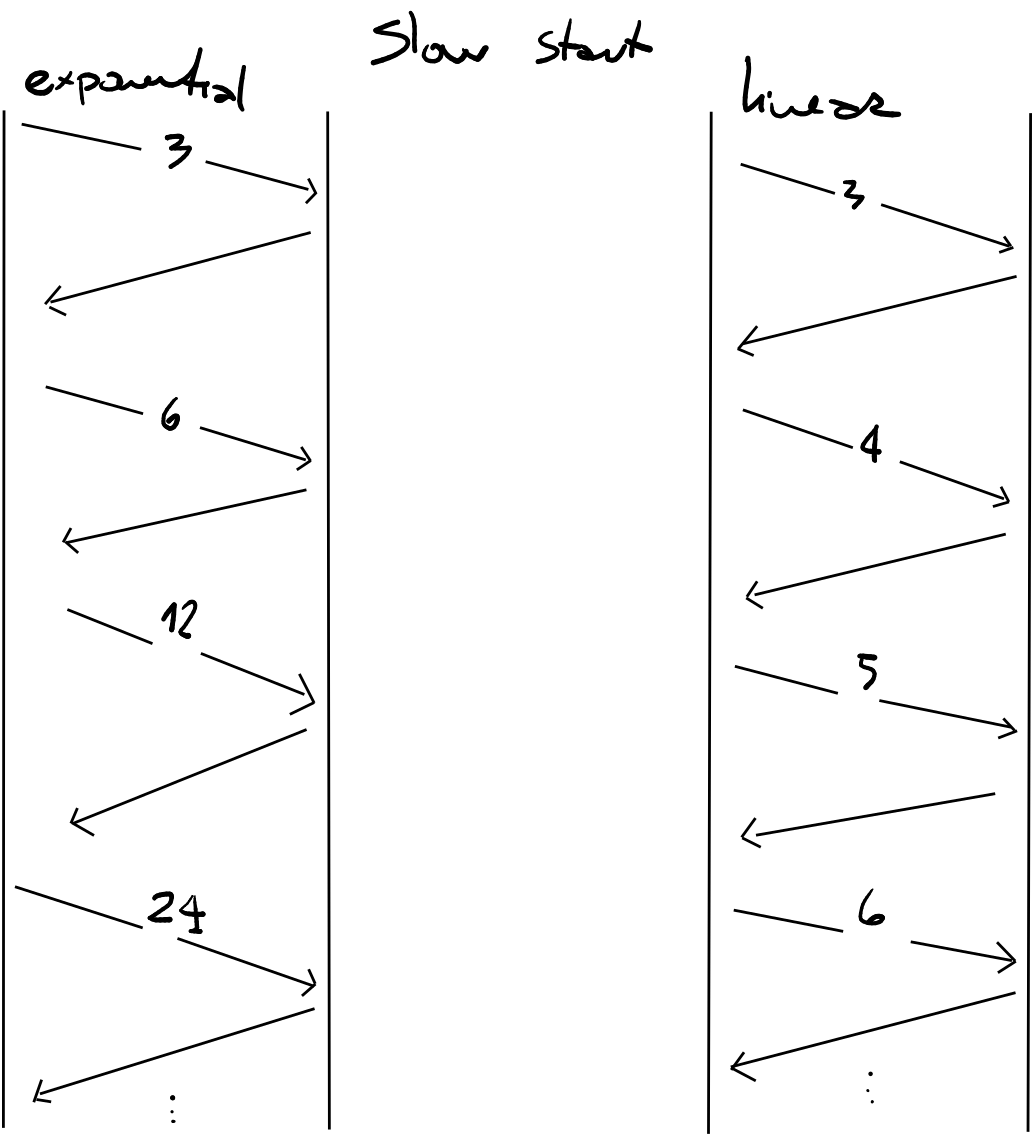
\includegraphics[ width=0.7\linewidth, height=\textheight, keepaspectratio]{./pics/tcp/slowStartTypes.png}
    \caption{The two kinds of slow start evolutions. At left, exponential, at
    right, linear.}
    \label{fig:slowStartTypes}
\end{figure}



\subsubsection{Congestion control and maximum throughput of the network}

What can happen on start?

Let's assume all segments are lost, and retransmission occurs after RTT (that
means, RTO is a good approximation of RTT). Let's also assume slow start
produces an exponential growth. Initial value of \emph{ssThresh\_start} is
$64KB$. Starting with threshold value below \texttt{T\_MAX}, slow start will
yield an exponential growth; after some time, congestion avoidance will enter,
a segment loss will occur and the congestion window will be reset to half the
\emph{ssThresh\_start} original value. 

Initial threshold above \texttt{T\_MAX}
will trigger a segment loss, and a reset of the threshold (without congestion
avoidance algorithm, that has not enough time to act). After the first segment
loss, threshold will be halved by setting it at half of the in-flight bytes,
and system will act as it started below the \texttt{T\_MAX} throughput. The
``exponential, linear, drop'' pattern will occur \emph{forever}, and the three
phases (slow start, congestion avoidance, loss detection) will happen one after
the other.

\begin{figure}[hb]
    \centering
    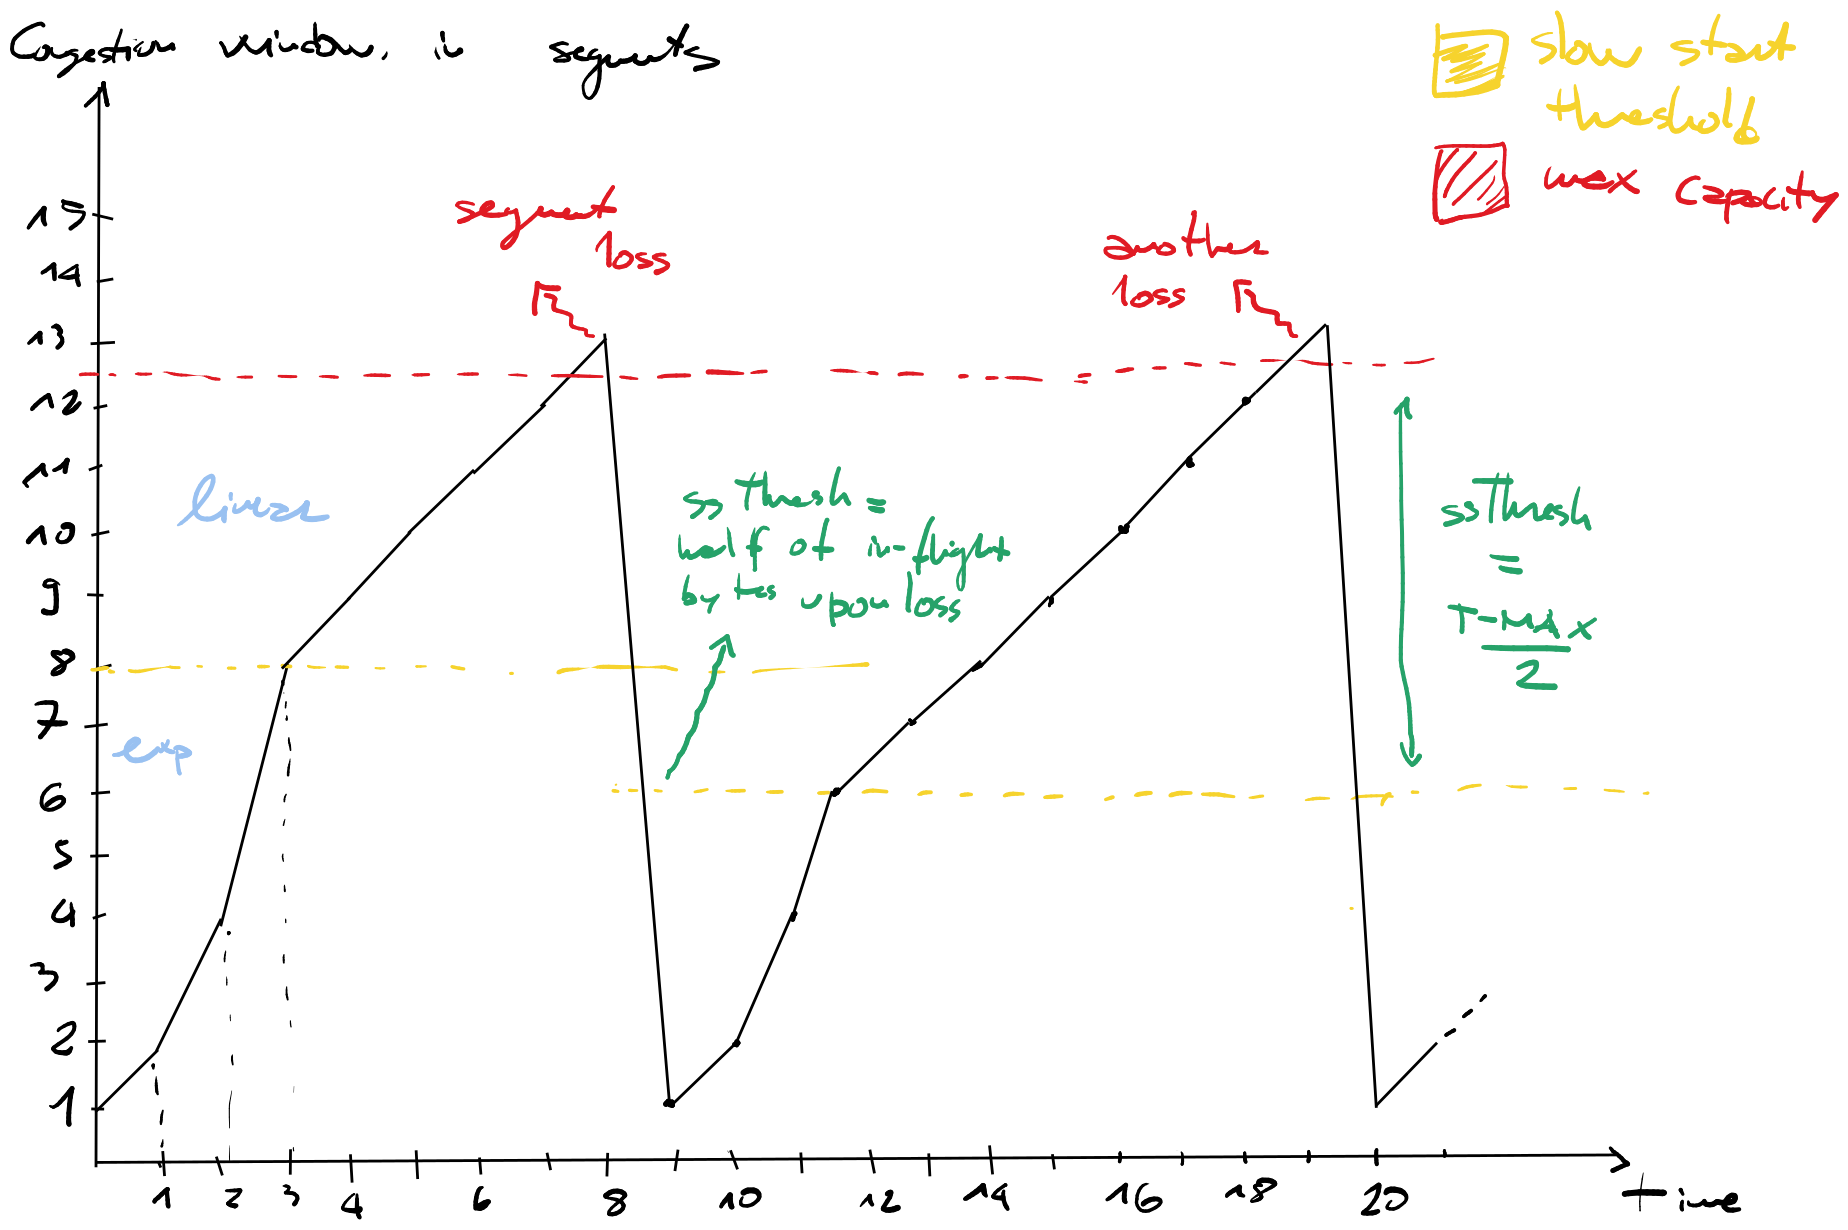
\includegraphics[ width=1.0\linewidth, height=\textheight, keepaspectratio]{./pics/tcp/congestionControl.png}
    \caption{Congestion control and its dynamics. The pattern indefinitely
    repeats.}
    \label{fig:congestionControl}
\end{figure}



\clearpage

With same assumptions as above, but with slow start provoking a \textbf{linear}
kind of growth, the pattern will be \emph{completely linear}, since no
exponential growth occurs. Basically, only the starting phase of each cycle
will be different. The end result in both patterns, however, is that the
average \texttt{T\_IN} value will be \textbf{much} smaller than \texttt{T\_MAX}:
the TCP congestion control cannot expoit internetwork capacity
efficiently. Injected throughput will always be lower than the maximum
possible: the consequence, is that the average throughput is lower than what
the network could sustain, however, this is very important in order to avoid
network collapse and congestion. 

There is a good reason for that: it is almost impossible to predict how the
network will behave. A network could host many devices, each one having
different demands, producing many kinds of traffic, each one with its own
\emph{volume}. The end result will be an unpredictable mess of network traffic.
The only way to adapt to this is to adopt an algorithm using a heuristic
behavior, that tries to adapt to the network as well as avoiding congestion the
most.

\subsubsection{Fast retransmit in a nutshell}

Suppose $K$ segements are transmitted in a burst, and a single segment among
them appears to be lost. Resetting the congestion window to its minimum value
is an inefficient move; since only a single segment of the row has been lost,
one could argue there is no need to drastically decrease the congestion window.

Another strategy could be \emph{waiting for a timeout before resetting the
congestion window}: the solution is inefficient too, since waiting before
retransmitting could lead to long breaks (how much to wait? how to estimate a
correct time interval?).

The \textbf{Fast retransmit} algorithm addresses precisely this kind of issue:
the solution is to retransmit \emph{immediately only} what appears to be the
missing segment, and decrease the window \emph{but not} to its minimum value
(that is, the maximum value between 2MSS and half of the current in-flight
bytes).

\subsubsection{Avoiding collapse of the network and the concept of fairness}

The congestion control slows down the network in order to assure both
\emph{collapse avoidance} and \emph{fairness}.

Intuitively, one would like to reach the maximum possible value for the
congestion window and the maximum throughput sustainable; however, both are
\textbf{unknown}. We can detect detect its value only after having injected an
excessive throughput, by detecing segment loss. However, whenever a segment loss occurs, the network is already congested. 

An aggressive slow down occurs
at each detection of segment loss, in order to prevent further collapsing of the
network. In fact, suppose many machines are injecting a throughput which is
closer to the maximum possible: in that case, if the network is congested,
\emph{it will require more time to return to its normal state}, because all
machines are insisting injecting throughputs close to unsustainable ones, and
removing congestion \textbf{will} require larger time. Basically, this is a
heuristic way to avoid congestion on a network where multiple machines are
using transmission resources altogether.

In the end, congestion control strives to ensure \textbf{fairness} with respect
to the other devices. Fairness is the tendency of each competing TCP connection
on a router to consume the same fraction of the router capacity. Each
connection, on average, will try to consume an equal fraction of router's
capacity. However, today's standard impose \textbf{node-level fairness}: this
means that each node should have the same amount of network capacity (thousands
of TCP connections can be opened at the same time from a single node). Note
that UDP connections \emph{do not} implement any flow or congestion control,
and transmit at full-speed: they are said to be `selfish'. 

Basically, the end goal of fairness is to grant anyone the same access of the
network, at the expense of your own networking speed (one could argue, however,
that if anyone tries to push as much traffic as possible in the network, no one
could be able to use the network, not even the same people that are pushing all
that massive traffic).

\subsubsection{Estimating the average throughput}

Some assumptions should be made in order to compute average throughput, given Congestion Control algorithm is running properly:
\begin{itemize}
    \item slow start has \emph{linear growth}. The congestion window starts
        from $1$ and goes up to $k+1$;
    \item \texttt{T\_MAX} is constant and in between $K\cdot MSS$
        and$(K+1)\cdot MSS$;
    \item \emph{all} segments are lost at once (no wild retransmissions);
    \item all segments are received up to $k$-th round; segments in round
        $k+1$-th are all lost at once;
\end{itemize}

The \emph{average throughput} that is injected is the average number of bytes in each
pattern, divided by $(K + 1)\cdot RTT$. The number of bytes in each pattern is
equal to MSS * number of segments in each pattern \-- since we are assuming a
linear growth, the segments are increasing linearly up to $k+1$, that means the
number of segments belonging to a pattern is $\frac{k \cdot (k + 1)}{2}$;
hence, the \emph{average throughput formula} is

$$A_t = \frac{MSS\cdot \frac{K(K+1)}{2}}{(K+1)\cdot RTT} = \frac{MSS\cdot
K/2}{RTT}.$$ 

Thus, the injected throughput is the same one would obtain by
having a \emph{constant window} of $K/2 \cdot MSS$ size \--- on average and
under ideal conditions, one can only get \textbf{half} of the maximum network
throughput.

Slow start in exponential fashion makes this calculation quite more complex,
but we will genuinely assume a linear growth in all our calculations, to make
them simpler.

\subsubsection{Idle connections}

Another important scenario that has not been disclosed yet is about \emph{not
transmitting data after many RTTs}, the case of \emph{idle connections}. The
basic idea is to reset the values of congestion window and slow start threshold
after a timeout expired (RTO).

Without a reset, one would use the last values that were determined by the
congestion control algorithm. In order to avoid bad performance, the sender
\textbf{resets both congestion window and slow start threshold} after a
timeout. Basically, by resetting the connection state regarding previously
achieved speed, the approach tries to be very pessimistic and conservative, in
order to avoid any kind of congestion in the network.

\subsection{Interaction between flow control and congestion control}

The interaction between the two TCP control systems is not straightforward.
After connection opening, the bound imposed by congestion control is
\emph{much} tighter than the flow control one (2--4 MSS instead of 64KB).

Hence, at the beginning the network \emph{will follow congestion control}'s
dictated bounds: data transfer begins slowly.

After connection opening (steady-state), there are two possible cases:
\begin{itemize}
    \item \texttt{T-MAX > T-FLOW-CONTROL} \--- when the maximum network
        throughput is greater than the maximum flow control throughput: in this
        case, the bottleneck is the \textbf{receiver's capacity}. The steady
        state throughput will be $\frac{M\cdot MSS}{RTT}$, while its connection
        opening transient throughput will be half of that value, that is
        $\frac{M \cdot MSS}{2RTT}$. What happens here is that there is a
        steady-state with a fixed value due to the flow control algorithm,
        while before reaching it and during the opening phase the speed
        increased following congestion control (slow start or congestion
        avoidance depending on how the slow start threshold has been initially
        selected);
    \item \texttt{T-MAX < T-FLOW-CONTROL} \--- when the maximum network
        throughput is lower than the maximum flow control throughput: in this
        other case, the bottleneck is the \textbf{internetwork}, and congestion
        window will go up and down, never reaching the value corresponding to
        the receiver's buffer size. The steady state throughput will be
        $\frac{K\cdot MSS}{2MSS}$. Basically, in this case the flow control
        never occurs, both receivers will never reach their full speed and the
        real culprit would be the internetwork.
\end{itemize}

Since the steady state during congestion control is variable and corresponds to
half of the actual internetwork speed, reaching a flow control steady state is
much more desirable, especially when the flow control window size is set
slightly below the maximum throughput. However, the exact \texttt{T\_MAX} value
is unknown and varies overtime, therefore it is impossible to reach such an
ideal scenario.


\subsubsection{Congestion control variants}

Many variants of Congestion control have been developed. In particolar, there
are many families for different use-cases:
\begin{description}
    \item[congestion collapse] this class attempts to increase the average T-IN
        upon congestion collapse in a standard, wired internetwork connection;
    \item[wireless] this class strives to optimize correct non-wired environments, with algorithms tailored to environments with high network loss;
    \item [high-speed] this class is tailored to sustain very-high bandwidth
        connections (e.g. backbones), with \emph{high bandwidth-delay product}.
\end{description}

The latter is the case of \emph{backbones}, with very-high bandwidth-delay
product \--- those are all the networks that, if TCP is left as default, will
lead to several minutes of connection start and gigabytes of data exchanged for
the sole goal of bringing the connection to full-speed! In order to optimize
them, several variants of TCP have been developed.

As an example, suppose a sustainable throughput $T_{MAX} = K \cdot MSS /
RTT$, and suppose the length of the first initialization period be $t_{init} =
K \cdot RTT$. Solving in $K$ leads to $$t_{init} = \frac{T_{MAX} \cdot
RTT^2}{MSS}.$$ By looking at the formula, one recognizes that the initial time
has a squared dependency over round-trip time, a direct proportionality over
$T_{MAX}$ and is inversely proportional to MSS. In all connections where both
RTT and $T_{MAX}$ are large or extremely large, the initialization time could
become relevant as well as the sheer quantity of the data that is needed (more
than $3$ minutes of transient, more than 100GB transmitted). For this reason,
variants of TCP for backbones are mandatory.

The following Table~\ref{tab:warmUp} sums up the values for some kinds of
connections, in the case of congestion control only.

\begin{table}[ht]
\centering
\begin{tabular}{r|cccc}
    & \textbf{\makecell{10Mb/s\\ 10ms RTT}} & \textbf{\makecell{10Mb/s\\ 2ms RTT}} & \textbf{\makecell{1Gb/s\\ 10ms RTT}} & \textbf{\makecell{10Gb/s\\ 10ms RTT}} \\
    \hline
    \textbf{MSS} & 536B & 536B & 536B & 536B \\
    \\
    \textbf{Maximum congWin} & 23 & 5 & 2332 & 23321 \\
    \\
    \textbf{\makecell{Congestion control\\ throughput (Mb/s)}} & 5 & 5 & 500 & 5000 \\
    \\
    \textbf{Transient} & 0.2s & $\sim$0.0s & 23.3s & 3.9m \\
    \\
    \textbf{Transmitted data} & 145.8 KB & 5.8 KB & 1475.6 MB & 145.76 GB
\end{tabular}
\caption{Warm up time for different kinds of connections, using the standard
TCP protocol with a standard congestion control. Notice the sheer number of
seconds required to warm up a 10-gigabit network and the unsustainable quantity
of transferred data when adopting the standard TCP protocol.}\label{tab:warmUp}
\end{table}
\bigskip

\subsubsection{Estimating the data exchange time}

Let \texttt{T\_MAX} be known and let $M$ the flow control window size be known
as well; $B$ bytes should be sent. To estimate the time of the entire data
exchange, a solution could be to first estimate the maximum number of bytes in
the transient phase, that is $$N = MSS \cdot [(\frac{M \cdot (M + 1)}{2}) -
3];$$ if the obtained quantity $N > B$, then the entire data exchange occurs
under congestion control. Otherwise, a portion $B - N$ of the bytes would fall
under one of the two possible steady states, depending on the relationship
between the maximum throughput of the network \texttt{T\_MAX}, and the window
size $M \cdot MSS$.

Notably, throughput in congestion control cannot be assumed to be exactly
$\frac{T\_MAX}{2}$ --- in fact, that is the average value over \emph{multiple}
periods, possibly many of them. In the case of a small value $B$ to delivery,
one could not have enough periods to assume the average throughput is the half
of the maximum throughput of the network.

Knowing \texttt{T\_FC} in place of $M$, one can easily find a solution by the
same means as above. However, one should take in account that in order to
understand whether the steady state lies in congestion control or in flow
control, one has to confront the throughputs so that only in the case of
$T\_MAX < T\_FC$ the steady state occurs under congestion control.

\subsection{Reliability of TCP}

TCP is a \textbf{reliable} protocol. The reliability in TCP only means that
exchanged data are received, in order, and with no duplicates.

A common misconception about TCP is that the \texttt{send()} system call
provides both delivery and reliability. Unfortunately, the \texttt{send()} call
only guarantees that the data has been handed to the underlying operating
system, without being able to tell whether the data has been successfully
delivered or not. In order to do so and achieve reliability, the application
must ask for data by invoking \texttt{receive()} --- the \texttt{receive()} call
will check whether there is a segment with a correct \texttt{ACK} or not.

Application layer invoking \texttt{send()} does not know how many bytes are
received by the other side of the connection. The \texttt{send()} call may
complete with no error, but no byte could have been transmitted \--- there is
no way to know how many packages are actually delivered to the other party.

Suppose the \texttt{send()} invocation ends with an error message.
Upon an error taken during the $n+1$-th send invocation, there is no way to
know if previous messages were actually delivered or not. Despite TCP being
reliable, there is \textbf{no guarantee} that messages up to $n$-th were
delivered and transmitted, since the error message for \texttt{send()} call
simply means there have been a failure in the TCP protocol, and data cannot be
handed over to the operating system.

The correct reasoning is that all bytes \emph{up to} $k$ are correctly
delivered, but one cannot know the exact value of $k$. 

Regarding bytes delivered to the application level at the other end, bytes were
received by TCP layer up to $k$ but probably $k - k'$ bytes \emph{are still to
be delivered to the application}. This means only a portion of them, $k'$, have
been delivered. Both $k$ and $k'$ are \emph{unknown}.

Hence, there is no exact possible reasoning on TCP when it comes to a
\texttt{send()} invocation, since application should call \texttt{receive()}
instead to be sure all the data up to $k$ has ben received.

Only after \emph{receive} call, with all ACK correctly received, one can be
sure that all previous data have been successfully delivered. 

Upon \texttt{receive()} or \texttt{send()} error, one \emph{cannot tell
anything about the previous \texttt{send()} invocations up to that
\texttt{receive()} call}, since there is no clue whether the packet has been
received correctly or not.

Any of these scenarios might be the reason for a \texttt{send()} failure:
\begin{itemize}
    \item \emph{not received}: packet never received by the partner;
    \item \emph{not delivered}: packet arrived, but partner crashed before
        reply;
    \item \emph{delivered}: packet delivered, but not reaching, connection is
        broken.
\end{itemize}

All these scenarios must be handled differently and correctly. Response to
failure should always be a correct failure handling and proper recovery from
damage, no matter its kind. Typical examples of error handling are:
\begin{enumerate}
	\item first, take an error;
    \item repeat the message;
    \item wait some time;
    \item send request again;
    \item do until receiving a response.
\end{enumerate}

However, this approach is often wrong. In fact, the party is repeating the same
request over and over, possibly producing an effect multiple times.

When dealing with financial transactions, same requests can be performed
multiple times, and lead to catastrofic errors and wrong operations. Only read
operations can be handled this way effectively.


\section{Opening a TCP connection}

\subsection{Sequence numbers initialization}

Opening a TCP connection involves the decision of the \textbf{starting sequence
numbers}, whose value is not necessarily set to $0$.

Upon connection opening, since they are not set to zero, each of the two sides
should agree to their initial sequence numbers. The ideal starting point is
that every \texttt{snd} pointer should be set to the same value, as well as the
other party's \texttt{rcv} buffer. 

A first idea could be to simply send initial
segments in which \texttt{snd.Next} are specified in header. Special segments
could carry a flag that denotes a connection request (from the client) and \texttt{OK}
(from the server). Both parties will set their initial \texttt{rcv} pointers
accordingly to the value read in the header from the other party. 

In reality, this first implementation suffers from many issues:
\begin{itemize}
    \item delayed duplicates from client may be received after a long time \---
        the server might uncorrectly believe another connection request is
        coming from the client (since there are port numbers, however, the new
        connection will be opened only in case the previous one has been
        closed);
    \item delayed duplicates from server may be received after a long time \---
        this way, an opening with wrong sequence numbers may occur. In fact,
        suppose a server initial \texttt{snd.Next} number is equal to $63$ and
        sent via a delayed segment. Now, if the server has sent another segment
        (which has not been delayed) with, let's say, \texttt{snd.Next} equal
        to $91$, the client would believe the server has chosen $91$ as the
        starting sequence number. This is not correct, indeed.
\end{itemize}

The solution to the above problems, in which delayed packets may be
undistinguishable from not delayed ones, is the ``\emph{cross your fingers}''
approach. Both machines \emph{assume} that a predefined, \emph{maximum segment
lifetime} exist, after which segments cannot exist. 

 The lifetime in question is named \textbf{Maximum Segment Lifetime (MSL)}, and
 it is arbitrarily set to $2 min$ ($120s$). After such MSL time passed, the
 machine simply assumes that the missing segment will never reach it. This is,
 in reality, wrong: IP do not have concept of \emph{time}, and packets are
 discarded only based off their number of \emph{hops}. Since the assumption
 does not match reality, the algorithm execution does not provide any
 guarantees --- it does, however, guarantee that no wrong duplicates may
 possibly reach the other endpoint.


\subsubsection{The three-way handshake protocol}

The sequence numbers are generated by the \textbf{ISN-generator} (initial
sequence number generator), a $32$-bit counter increased every $4\mu s$, even
when the connection is switched off. Overflow will eventually happen every $4$ to $5$
hours. The generator is used to generate an initial sequence number from its
current value; a sequence number can be used again after at least $4$ hours,
after the ISN-generator will overflow.
\begin{figure}[b]
    \centering
    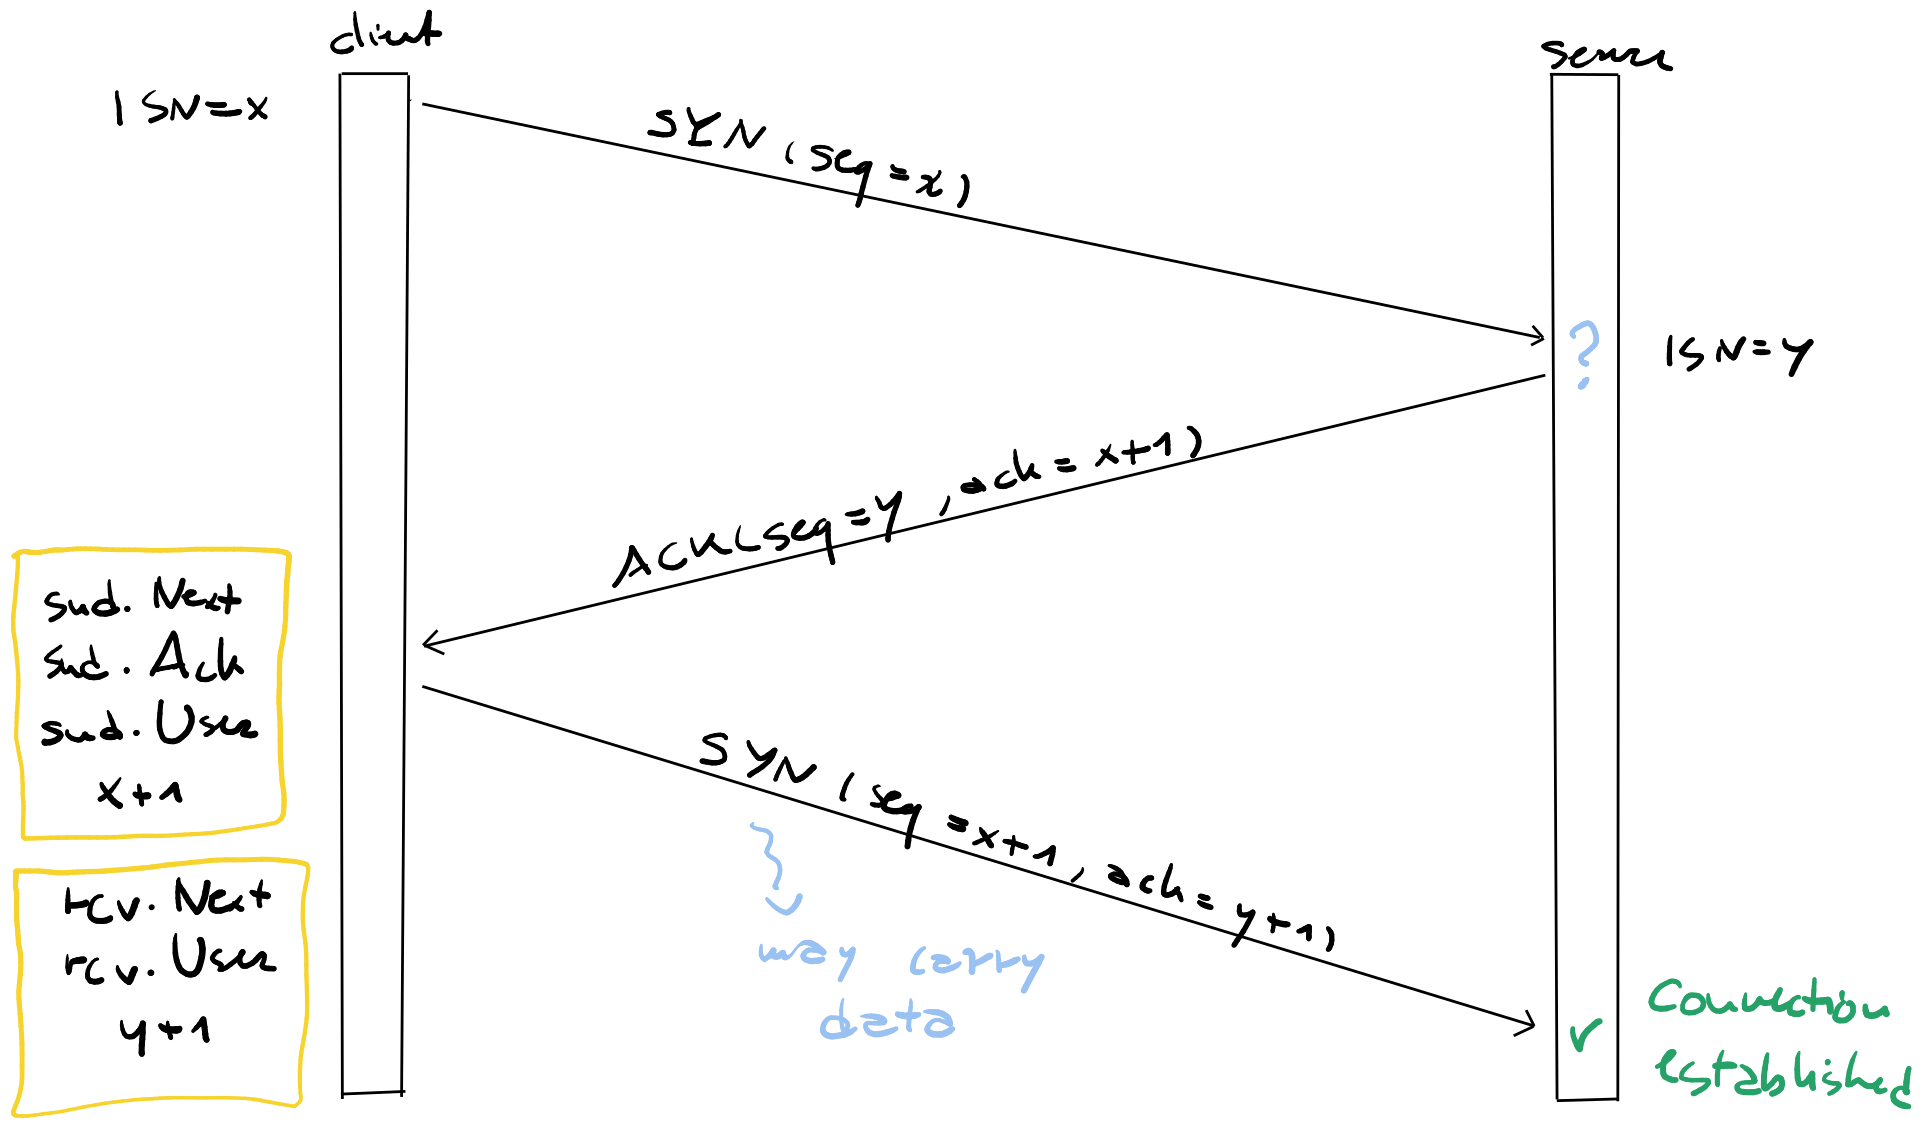
\includegraphics[ width=1.0\linewidth, height=\textheight, keepaspectratio]{./pics/tcp/threeWayHandshake.png}
    \caption{The three-way handshake.}
    \label{fig:threeWayHandshake}
\end{figure}

Upon connection opening, the initial sequence number will be obtained by
querying the ISN-generator.

The three-way handshake protocol (Figure~\ref{fig:threeWayHandshake} will begin
with sequence number initialization, whose value has been obtained from the
ISN-generator (suppose it's $x$), and send a \texttt{SYN(seq=x)}\footnote{SYN bit is a
flag in TCP header that is always zero, except in the first and second
segments, and it is used only for requesting connections.} packet to the
server. The latter will answer with a package such as \texttt{SYN(SEQ=y,
ACK=x+1)}, signaling both server's initial sequence number and that it has been
acknowledged bytes up to $x$, and it is ready to receive the next (actually the
first) byte.

The client will then respond with a second
message, containing data and having sequence and acknowledgement numbers
\texttt{(SEQ=x+1, ACK=y+1)}, showing that it is ready to receive the first byte
after $y$ as well; now, connection has been established and both parties will
assume the connection is successfully opened. 

The client side will be sure that no delayed duplicates are coming, otherwise
$x$ would have come from a connection which has been opened more than $4$ hours
ago! The same reasoning happens from the server side: any delayed duplicate
should have been traveling for more than $4$ hours, which is almost impossible
to happen. 

This protocol even protects in the case \emph{old duplicates} are delivered to
a server: in that case, the server will open a connection since the request looks legitimate. However, when the client receives the packet from the server \--- for
something they did not request at all \--- it will respond with a
\texttt{REJECT} packet\footnote{\texttt{RST} is a header flag as well as
\texttt{SYN}, and it is used only to reject connections.}. The server will
finally answer with a \texttt{REJECT(ACK=y+1)} to signal it has correctly
acknowledged the request to close the connection.

A very unlucky case is where the server receives two delayed duplicates, one
coming to open a connection and the other one just after the server sent its
\texttt{ACK}; however, there is little to no chance that the ACK values are
correct (and, in that case, it would have traveled for more than $4$ hours,
much more than MSL value of 2 minutes). In fact, in those cases, rogue packets
from a client would contain \texttt{CR(seq = x)} and \texttt{DATA(seq=x+1,
ack=z)}, with the server expecting an acknowledged sequence number \texttt{y}.
The same goes if the server receives a \texttt{REJECT} (it cannot be a
duplicate). The mechanism is shown in Figure~\ref{fig:threeWHduplicates}.

\begin{figure}[b]
    \centering
    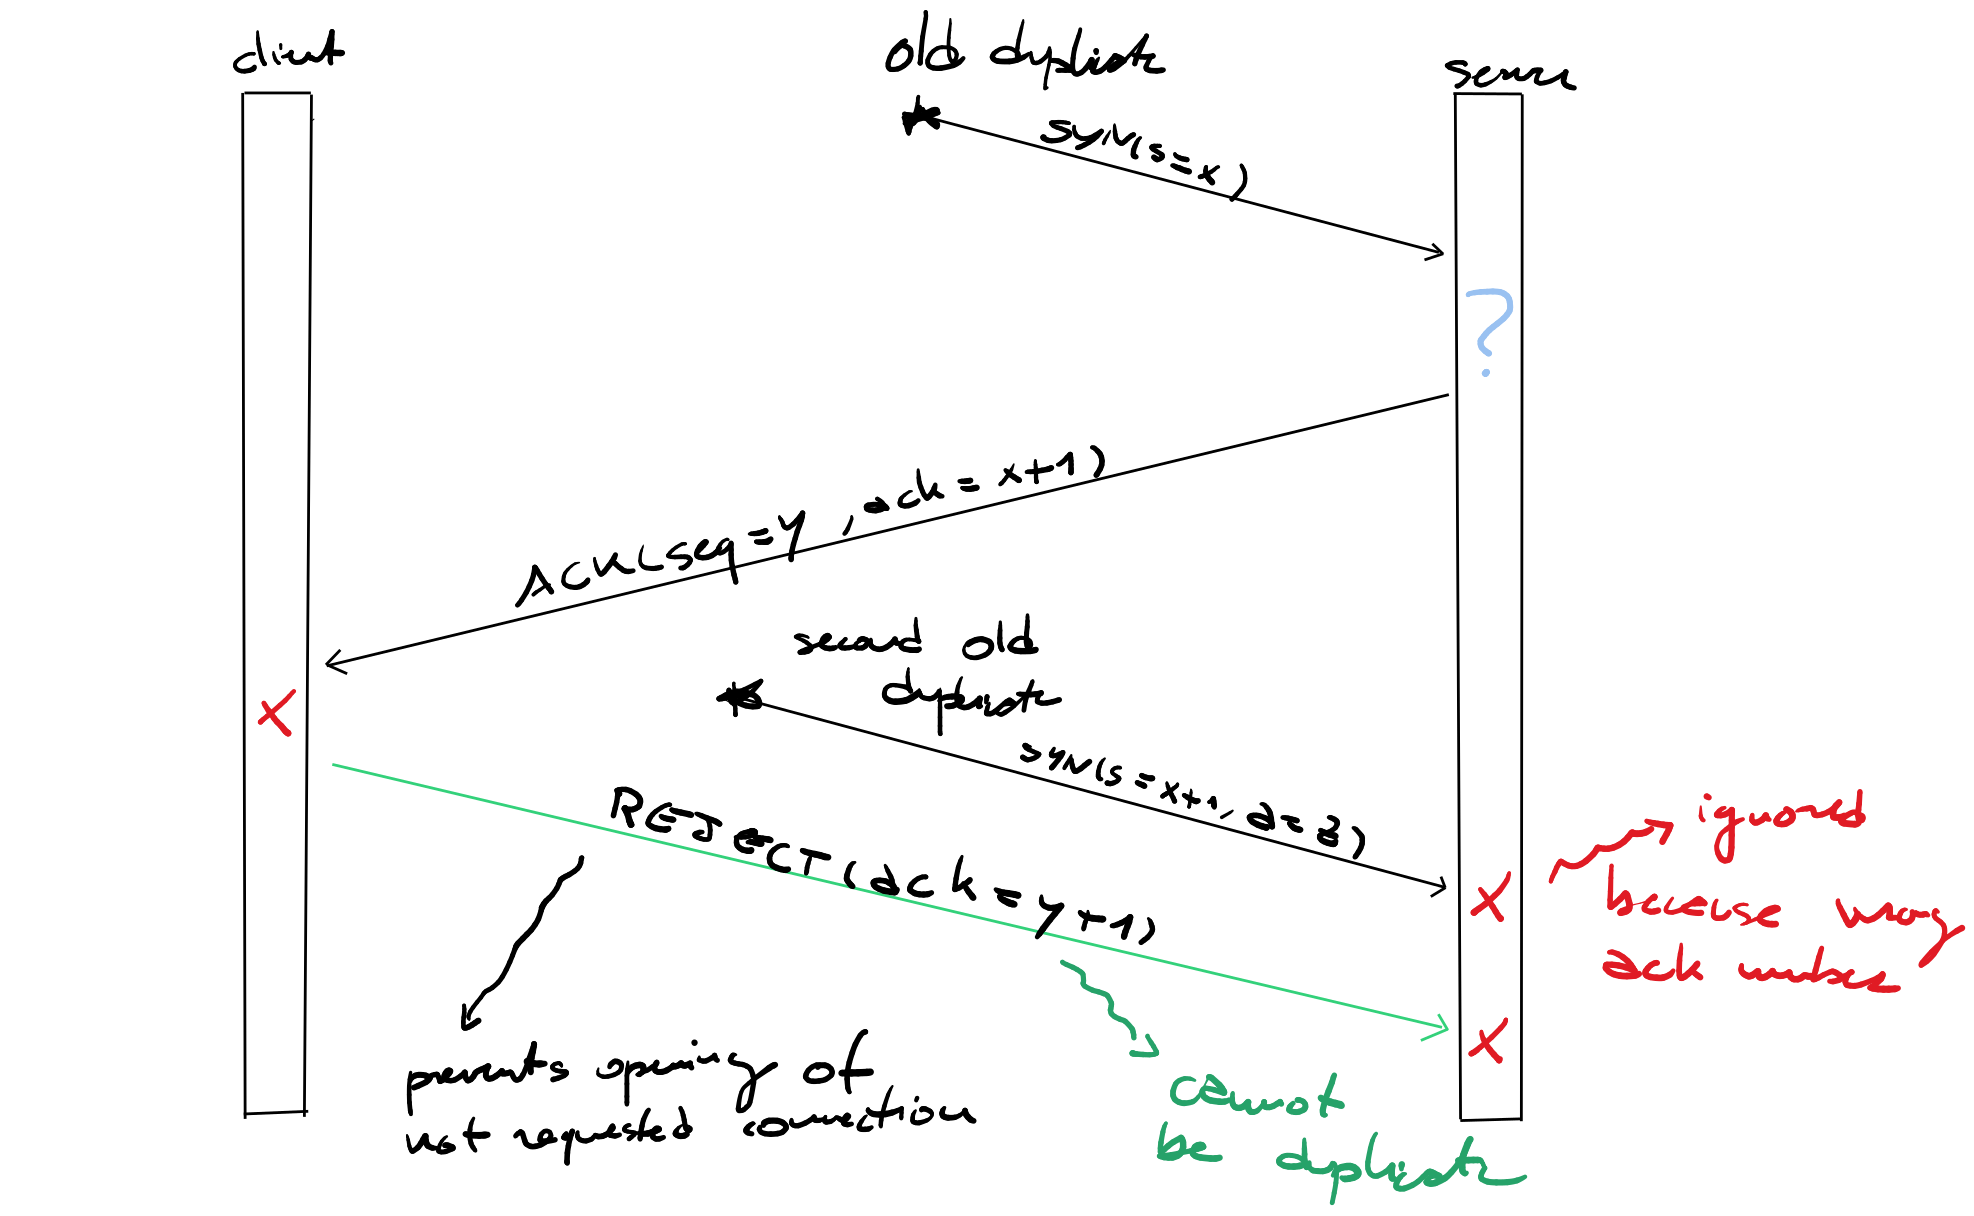
\includegraphics[ width=1.0\linewidth, height=\textheight, keepaspectratio]{./pics/tcp/threeWHduplicates.png}
    \caption{Possible errors in TCP handshake. The TCP protocol and its
    sequence number system is designed to avoid unsolicited connection opening,
preventing the server to waste resources with no reason.}
    \label{fig:threeWHduplicates}
\end{figure}



As we have already said, \texttt{RST} flags are used to reset a connection, or
close an unwanted one. \texttt{RST} segments should be sent in two cases,
\begin{itemize}
    \item unexpected \texttt{rcv-seqnum} in 3-way handshake;
    \item received segment for closed connection;
\end{itemize}
and in those cases, the \texttt{RST} segment is sent with the sequence number that is
expected by the peer.

In case the \texttt{RST} packet is legit (that is, when it carries the sequence number
the machine expects), then \textbf{close} the connection and \textbf{ignore}
\texttt{rcv-segment}.

\subsection{Interface between 3-way handshake and application layer}

To open a connection, application layer just requests TCP to open a connection.
The TCP layer will handle the connection opening with the appropriate system
calls, with the protocol as described above.
The system calls in sequence are

\begin{itemize}
	\item \texttt{socket};
    \item \texttt{bind};
    \item \texttt{listen(num, ...)};
    \item \texttt{accept}.
\end{itemize}

System call \emph{listen} has a \emph{num} in argument that tells \emph{how many
connections can be queued}, that is, the number of incoming \texttt{SYN} segments that
should be queued before opening connections. Until \texttt{listen} call has
been invoked, no connection can be opened and the server will respond with
\texttt{RST}. Up to \emph{num} \texttt{SYN} segments can be accepted at the
same time \emph{before} invocation of accept and delivery of \texttt{SYN-ACK}
packages. For instance, if \texttt{num=5}, the server will wait for $5$
connection requests before actually answering to the client and opening the
connections.

Closing a connection is done with the \texttt{FIN} flag. It is handled the same
way as \texttt{SYN} is, and where one party wants to close connection, sets
\texttt{FIN} flag to $1$ and the other party will respond with a \texttt{FIN}
flag to $1$ as well.

This protocol can be abused to block a server with little to no effort. Attacks
whose goal is to prevent the target working are called \textbf{Denial of
Service} attack. An example of DoS attack is the \textbf{SYN-flood} attack.

The idea is to keep sending \texttt{SYN} segments so that server queue \emph{is
always full}: the effect will be that legitimate \texttt{SYN} requests from
legitimate clients will be discarded. Some variants even hide the
\texttt{IP-src} by modifying it, in order to hide attack origin. This way, it
is impossible for a defender to prevent the SYN-flood by blacklisting IP
addresses. Moreover, \texttt{SYN-ACK}s responses will be delivered to (fake)
IP-src address.

SYN-flood attacks are very hard to detect and very cheap to operate.
Indeed, randomly forging \texttt{IP-src} addresses makes almost impossible to
filter them out with a firewall. SYN-flood attacks are also cheap: for $128$
opened connections every $3$ minutes, only $128\cdot 40 = 5120B \mbox{ every }
180s = 228 bps$ bytes are needed to the attacker to forge necessary packets. To
forge $1280$ connections, $1280\cdot 40 = 51200B \mbox{ every } 3 m = 6826bps.$
A small cost of sending a packet causes the listener to force a listening to a
connection, a \textbf{much} higher cost. 

By designing a new protocol, one would likely avoid spending resources upon the
first \texttt{SYN}, by operating \emph{statelessly} until the initiation can
demonstrate its legitimacy. However, a new protocol is almost impossible to
design, since existing network architectures cannot simply be replaced.


\chapter{Threat model}

\section{Understanding threat model}

TCP offers \textbf{no authentication mechanism}. It means that if, for example, the
address has been maliciously altered in DNS, a connection can be opened to the
attacker's service rather than to the legitimate one and the client would not
notice the difference. Network attacker may be in control of the router, too
\--- he might be capable of switching DNS requests and respond with fake
responses.

TCP offers \textbf{no integrity mechanism} either. A network attacker might
change what the machine sends and receives \--- a communication may be altered
by an entity that acts in between the two legitimate parties. Fortunately, an
improved version of TCP, \textbf{TLS (Transport Layer Security)}, is available.
It works by acting on top of TCP, and uses \emph{cryptography} to provide
integrity to protect the message and offers a strong authentication mechanism.

However, TSL can still be compromised: Suppose in fact the client has been
infected by a \emph{malware}\footnote{A \emph{malware} is a malicious software,
secretly installed by the attacker and against the user's consent, to perform
ill--intentioned behavior} --- then the attacker can control the client's
behavior from remote, for example modifying web pages, opening connections,
attempting privilege escalation\footnote{\emph{Privilege escalation} is a
technique in which an attacker that has gained unprivileged access to the
machine tries to obtain super--privileged access by means of exploits,
vulnerabilities and by other techniques. For instance, an attacker could try to
obtain \emph{root access} and root privileges to perform anything he wants on
the machine.} on the machine. In this case, TLS does not guarantee secrecy,
integrity, authentication.

An crucial question arises: \emph{is then TLS vulnerable and therefore pointless?}

Basically, it all depends on \textbf{threat model}. A threat model is the set
of actions that \emph{we assume the attacker can execute}. One makes an
\emph{hypothesis} on the set of attacks that are possible, and then it reasons
accordingly. In fact, reasoning about security of a system without a well-posed
threat model makes no sense at all, because an attacker that doesn't have a
predefined set of attacks and can do anything is an attacker it is impossible
to defend against. That said, a \emph{real attacker} may not be confined in a
single, limited, threat model, because it both may be modeled unaccurately and
it may be unpredictable.

An important remark is that all protections in software are designed with a
specified threat model in mind. They do not work outside their threat model
which they are based on, and for this reason software should be chosen
accordingly. Both protections and possible kinds of attackers are important to
be established before acting, in order to minimize expenses, maximize defense
capabilities, and increase the chance an attacker is successfully repelled.

Important questions when dealing with attackers are the following ones, 

\vspace*{1cm}
\setsansfont{Heliotrope 4}
\begin{quote}
\begin{center}
    \sffamily {What's the \emph{threat model} for that specific attack technique?

\bigskip
    What's the \emph{least pessimism} required in order to execute an attack?

\bigskip
    What's the \emph{best software} in terms of \emph{cost}, \emph{defensive
    capabilities} and \emph{chance to be attacked} that should be used to
defend to a given attack?}
\end{center}
\end{quote}
\bigskip
\setsansfont{Concourse 6}

Typical threat models involve the following scenarios, in increasing pessimism:
\begin{itemize}
    \item \textbf{Network attacker} \--- the attacker can only operate in the
        network. He is able to observe and communicate. DoS (Denial of Service)
        and MITM (Man in the Middle) attacks are usually what a network
        attacker can do;
    \item \textbf{Compromised endpoint} \--- the attacker compromised a node in
        the network with a malware. That node is fully compromised and should be
        considered not trusted;
    \item \textbf{Physical access} \--- the attacker obtained physical access to an
        endpoint. Regardless of the fact a machine is already infected or not,
        physical access grants much more privileges than the above threat models,
        for instance it can compromise much more easily an endpoint or can
        install devices that are physically capable of acting as man in the
        middle;
    \item \textbf{Evil maid} \--- a \emph{variant} of both \emph{physical
        access} and \emph{insider} threat models in which an person that has
        frequent physical access to a machine is instructed to perform
        operations on the device. An evil maid has no access on supply chain or
        organization internals, though;
    \item \textbf{Insider/Supply chain} \--- this very dangerous attacker has
        access to portion of the \emph{software supply chain}, for instance it
        can manipulate software libraries the main software depends on,
        infrastructure on which the software development occurs, and so on. In
        the case of the insider, it also has access to the internal
        communications and is able to actively spy the organization he is into.
\end{itemize}

The TLS (and by extension, the HTTPS protocol) grants \emph{secrecy},
\emph{integrity} and \emph{authentication} only for a network attacker--based
threat model. Outside that model, TLS and HTTPS offer no guarantee of
protection.

\subsection{Choosing the defenses}

Threat models are also useful to define from which kinds of attacks one should
defend, from which ones one cannot defend and should act accordingly, and from
which ones one simply has to ``cross his fingers'' (do nothing).

The first category of attacks should be treated with proper software that
offers protection against a well--defined threat model. Outside that model, the
software should be considered useless and the system that it protects is
compromised and not anymore trusted. This category of attacks is rather
frequent, doesn't cost too much, and poses immediate danger to the activity of
the organization. 

The second category, whose best defense is \emph{damage compensation}, is the
category of attacks that are not very frequent and whose relative defensive
mechanisms cost too much to be economically viable and sustainable for the
defending organization. In these cases the organization simply prepares for
damage mitigation, with strategies such as \emph{data backups}, \emph{backups
of systems} and by other means.

The third category is both rare and costly. These kinds of attacks are very
dangerous, but occur extremely rarely. It is therefore rational to simply allow
this kind of risk to happen, without taking any countermeasure in account.

An crucial remark is that for \emph{choosing the defenses}, it is not important
\textbf{how} an attacker has managed to operate an attack, and it suffices to
know the specific threat model and attack set an attacker is able to conduct.
For \emph{assessing likelihood} of a threat model, in order to decide the
actions to take, it suffices to know how an attacker has been able to achieve a
certain attack capability.

In fact, the details on how an attack works and how it is only necessary to
find and determine the cause of a given vulnerability or exploit.

The first step of a defender should be to determine a threat model by looking
at how simple is for an attacker to achieve a certain specific attack. The next
step is to determine the best defenses \emph{given} a threat model.


\subsection{The network attacker threat model}

The \emph{network attacker} threat model is implicitly assumed in this book. A
network attacker can only operate in the network, by communicating, observing
and altering existing traffic. An attacker of this kind cannot act on the
endpoints.

The implicit assumptions are that everything on the endpoints is perfectly
implemented, operated and maintained --- this means that there are no
vulnerabilities, no exploits, and no obvious mistakes by the system
administrator. Software is perfectly maintained as well. No mistakes are
allowed, no remote code execution, no vulnerability, no mistakes from the
users, in cryptography, protocols and communication, and operating systems.

These kind of assumptions are important to confine the attacker to the network
threat model; otherwise, an attacker could be able to infect an endpoint,
upgrading the threat model to the \emph{compromised endpoint} threat
model.

The key defensive tool against a network attacker is \textbf{cryptography}.
Cryptography allows both \emph{secrecy} and \emph{integrity}, and by means of a
structured trust system it allows \emph{authentication} as well. All of these
protocols make use of cryptography:
\begin{itemize}
    \item TLS and HTTPS;
    \item Kerberos;
    \item Windows Active Directory;
    \item OAuth (SPID);
    \item SSH;
    \item IPSec;
    \item Legally binding digital signature;
    \item WhatsApp, Signal, Telegram;
    \item and so on.
\end{itemize}

Examples of possible attacks a network attacker is capable of are listed below,
\begin{itemize}
    \item \textbf{DNS Spoofing} --- a DNS attack in which an attacker modifies
        the IP address (and the ID in header) contained in the response to a
        DNS query, in order to hijack a client to an attacker controlled
        server, and act as man in the middle, or showing a perfect copy of
        another website. Windows systems are particularly vulnerable to this
        kind of attack, since by default they prefer any IPv6 server and
        happily substitute the preconfigured IPv4 server upon a malicious
        packet containing new instructions arrive;
    \item \textbf{ARP Spoofing} --- fake responses crafted by an attacker, whose
        goal is to make a device change its default gateway to an attacker's
        controlled device, so that it can act as man in the middle. Open WiFi
        is vulnerable to this kind of attacks;
    \item \textbf{BGP Spoofing} --- highly--skilled attack in which an attacker
        manages to alter the routing of the internet, so that it can direct
        traffic to different places. Border Gateway Protocol messages are not
        authenticated; Autonomous Systems can claim ownership of any IP
        address;
    \item \textbf{Dishonest system administrators} can act as man in the middle;
    \item \textbf{Judicial authorities} or \textbf{intelligence agencies}
        possess huge available resources, and can force organizations, internet
        nodes and system administrator to act as man in the middle.
\end{itemize}


\section{Attacking TCP connections}

A legitimate threat model for a TCP connection is the network attacker threat
model. A network attacker can observe, communicate and alter traffic by acting
as man in the middle in all communications between two endpoints.

The first model of the network attacker that strives to control a TCP connection
is the \textbf{on--path attacker}. The on--path attacker is able to read
integrally the communication between the two endpoints, and can act as man in
the middle.

The objective of the first kind of attack we will encounter is the \emph{client
impersonation} in a TCP connection between a client and a server. The server
will see the IP of the client at the other end of the communication, whilst
packets are actually sent and received by the attacker.

There are three possible ways to perform such an attack:
\begin{enumerate}
    \item \textbf{Opening a connection} and impersonating the client's IP
        address;
    \item \textbf{Injecting some data} in an already opened connection;
    \item \textbf{Closing a connection} already running.
\end{enumerate}

In the second method, the attacker only injects \emph{part} of the
communication, and represents a less pessimistic approach, in which the attack
does not manipulate the communication and can only inject data. The third
method is the more optimistic one, with the attacker only capable of closing an
existing connection in order to perform some kind of Denial of Service.

All three attacks are trivially feasible, with an attacker able to act as man
in the middle. In the first case, the attacker is able to intercept an opening
connection, and starts handshake with the server, opening a connection.

An on--path network attacker is able to intercept all segments. In particular,
such attacker is interested in obtaining sequence numbers, so that it can
successfully replicate the connection state, inject data, and manipulate
correctly the connection by means of forged segments with correct sequence
number.

Data injection by an attacker cannot happen at an arbitrarily high rate.
Attacker must forge correctly numbered segments, so that both the client and
the server could not notice the manipulation. This in the past was a tremendous
issue, since there were big problems with remote shells from clients
authenticated by IP --- today it poses no longer a problem, since authentication
occurs almost always by encrypted protocols such as \emph{SSH (Secure Shell)}.
Injecting data is easier at TCP level, with carefully crafted headers and
proper payload; backwards, data injection at application layer is much harder,
since an attacker must know application protocols and expected data at time
$t$. This, however, is feasible: the \emph{National Security Agency} has done
it many times in the past, in a highly targeted way, with web browsers driven
to web servers that inject malware, by means of injecting HTTP redirect in HTTP
responses.

Attacker can also close a running connection. All he has to do is to send a
single \texttt{RST} segment with correct sequence number to be accepted by the
server, and the closing procedure will start. Closing a connection is really
feasible: a sequence number can be easily inferred by looking at the incoming
sequence numbers, and to increase the likelihood of picking the correct
sequence number, \emph{many} forged segments are sent with sequence numbers
that are likely to be the correct ones.

The second kind of TCP attacker is the \textbf{off--path attacker}. An
off--path attacker is less powerful than the on--path attacker, since it is not
in the path and thus cannot read the correct sequence numbers.

An off--path attacker is \textbf{not} able either to open a connection or to
inject data. However, despite the deep limitations in what he can do, he is
still able to \emph{communicate} to each endpoint and this suffices to be able
to close a connection and perform other kinds of Denial of Service attacks.

The attacker's objective is to determine the client information regarding \emph{sequence number} and \emph{port number} at time $t_x$: the two informations suffice to close a connection easily. The procedure is as follows:
\begin{enumerate}
    \item to begin with, the \emph{correct sequence number} should be estimated by
        means of stochastic techniques;
    \item the \emph{client's port number} is determined as well, by means of
        stochastic techniques or by looking at the default numbers;
    \item for each pair of \emph{possible candidates}, send a \texttt{RST} segment to
        the server.
\end{enumerate}

To determine a possible candidate, the idea is to first get the current initial
sequence number from the client, then estimate the amount of data exchanged by
the TCP connection, so that by adding the estimated amount one could obtain the
initial sequence number at the time and choose the candidate in the most promising range.
The initial number is obtained by a fraudulent connection opening with the
client, so that the initial sequence number can be obtained; if the
\emph{slope} of the initial sequence number generator is known at the time
interval \texttt{t} (that is, if one knows \texttt{ISN@C(t)} and how \texttt{ISN@C}
behaves he can estimate \texttt{ISN@C(topen)}), the attacker can make a guess
on the \emph{starting} sequence number the client employed. After that,
estimation is based on the application protocol and the total number of bytes
sent can be guessed. A \emph{range of likelihood} for sequence number is
determined, and finally as many segments as possible are sent to the server,
hoping for the best.

The power of this method lies in the sheer computational power of the attacker.
If the attacker is able to produce a huge number of sequence number and port
number candidates to forge enough \texttt{RST} segments in a sufficiently tight
time interval, the server could end up accepting the fraudulent close request,
determining the closing of the connection. This results in a powerful method
for Denial of Service, for any kind of existing TCP connection.

Historically, in 1985 people started realizing what \emph{could} be done
against TCP initial sequence numbers; there were no proof of concepts, however.
The first real attacks were performed in 1995, and pushed the widespread
adoption of pseudo--random number generators that should be addressed by the
TCP algorithm in order to determine its initial sequence number. Basically,
that made apparently impossible for an attacker to determine the correct
sequence numbers. That said, in 2001 attackers were still able to determine it
by means of \emph{statistical techniques}, so people realized that the widely
adopted algorithm were suffering from vulnerabilities and design failures. The
number of attempts for succeeding was much smaller than the amount that was
believed to be necessary for the attack to work; clever bruteforce was
feasible. In 2001, a new algorithm was built in order to make the initial
sequence number choice unpredictable. Unironically, in 2004 attackers were
already able to produce efficient Denial of Service attack, since the required
number of attempts was sufficiently small to be feasible.

The lesson learned is that even if \emph{today} realistic threat models assume
that a certain attack is not possible, \emph{after some years} someone realizes
that the assumption is wrong; this is due to the fact that resources, knowledge
and techniques vary over time.

The same fate struck the WPA2 protocol; designed in 2004, a serious weakness
uncovered in 2017 allowed an attacker to read, inject and manipulate data in
the encrypted protocol. Since the weakness was in the standard itself, any
correct implementation of WPA2 was likely affected.

In 2014, off--path data injection became possible as well. On HTTP, it is now
possible to insert \emph{scripts} and \emph{HTML segments} in a communication,
just by sending packets to an endpoint.

\section{The Man--On--The--Side attack}

A \textbf{Man--On--The--Side} attack is an attack in which an ``observer''
network attacker attempts to hijack the web browser of the target to a website
controlled by the attacker, with the goal of injecting exploits on the victim's
browser.

To do so, an attacker first intercepts the HTTP request, and \emph{immediately
sends back} an HTTP redirect, with the sequence number expected by the victim's
browser. The latter performs the redirection to the attacker's controlled
website, with an HTML document forcing the download of many exploits.

The legitimate response from the server will arrive later, thus appearing
\emph{duplicate} and it will be discarded by the victim's browser.

This kind of attack is very powerful if performed by intelligence agencies,
usually with the help of Internet Service Providers.

Man on the side attacks are fully prevented by HTTPS protocol.

\chapter{Network Address (Port) Translation}

In networking, some IP addresses are \emph{reserved}. Among all the possible
addresses, there are 4 ranges that cannot be assigned to any ``public'' entity:
\begin{enumerate}
    \item the \texttt{10.0.0.0/8}, $2^{24}$ addresses in total;
    \item the \texttt{172.16.0.0/12}, $2^{20}$ addresses in total; 
    \item the \texttt{192.168.0.0/16}, $2^{16}$ addresses in total; 
    \item the \texttt{224.0.0.0/4}, $2^{28}$ addresses, reserved for
        \emph{multicast}.
\end{enumerate}

Addresses belonging to the first 3 ranges are said to be \textbf{private} IP
addresses, in contrast to the \textbf{public} IP addresses. The first addresses
belong to the internal network of a single organization, while the second
addresses must be purchased from an ISP, or publicly purchased from some
governative organization, and they cannot be assigned autonomously. The number
of devices is much greater than the number of available public IP addresses.
Private network numbers are then necessary in order to manage the network of
organization. A private IP address is unique only in the boundaries of a single
organization.


As a general networking rule, every frontier router must discard incoming or
outgoing packets with private IP addresses. This means that each and any device
possessing a private IP address cannot communicate directly with any IP address
outside an organization, and it has IP connectivity only with nodes internal to
the organization. Since nowadays it is very important to be able to communicate
externally (many applications do require direct internet access), a different
communication mechanism for devices with private IP addresses should exists.

To achieve the goal, there are two different technologies with similar
functionalities, but different implementation. The first is the \textbf{NAT},
Network Address Translation. The network address translation is no longer used.
The second one is called \textbf{NAPT}, Network Address Port Translation, and
it is usually shortened with \emph{NAT}. NAPT is what's used today on gateway
routers.

\section{How NAT works}

The basic idea of \textbf{NAT} is to \emph{modify the header of a packet} so
that the private addresses are replaced with a public address, and the port is
changed accordingly. Suppose a device with private IP address
\texttt{192.168.0.1} is trying to connect to \texttt{4.26.18.144}, a public IP
address, on port 777. The packet will travel to the default gateway, our NAT
device. The NAT will then inspect the packet, look for address and port
information in header, and \emph{modify them} so that the source IP address now
is the public IP address of the router (let's say, \texttt{80.68.17.190}), and
the port number is changed with an on--the--fly generated port number that is
currently available (suppose 18923 instead of 777). Basically, a NAT devices
alters IP address and port information of a TCP and UDP packet and maps them
into the public address of the router \emph{plus} a port number which
corresponds to the device that is requesting the connection. NAT module will
also modify the \emph{header checksum}, reconstructing it in order to match the
new packet that has been built (otherwise, all modified packets would be
discarded within the next hop).

All a NAT module should do is to remember for some time that the device packet
has been mapped to a specific public IP address (all devices will be mapped to
the same one) and port number. Each time a packet from the inside travels
through a NAT, a new device---port number mapping is produced and stored in a
table, the \textbf{NAT Mapping Table}. The mapping table stores all the
mappings across time. After a time interval, a mapping is discarded.

Upon new connection from inside to outside, NAT will look at the mapping for
translating \texttt{IP-I, port-I} to \texttt{port-E}. If there is no existing
entry, choose unused \texttt{port-E} and allocate the entry in the mapping
table. After that, modify all TCP/IP headers according to the table.

When a packet from the outside comes to the NAT module's external interface,
NAT device will inspect both the packet header and its own mapping table: if a
correct mapping exist, packets with the correct public IP address as recipient
will be delivered to the correct recipient \emph{inside} the organization;
which device, it depends on the mapping between the port number and the
internal device. Basically, incoming data are translated back again by means of
the \emph{same} association in mapping table. Such translation at both sides
will result in packets correctly delivered to their destinations.

A very important aspect of the NAT translation is the way that a NAT module
\emph{protects the network}. In fact, \textbf{any} packet, request or access
from the outside for which an existing association does not exist, \textbf{will
be discarded}. This is a crucial facet of a paramount importance: one of the
most important defense mechanisms is to avoid access from the outside; by using
a NAT module, one is able to immediately obtain network insulation from the
outside, for free. For this reason, NAT is said to be \emph{``a native
firewall''}. All of this does not require change or configuration on internal
nodes, they only need to set up a proper gateway --- address translation happens
to be \textbf{transparent} to the clients.

NAT modules can be configured with \textbf{immutable entries} as well.
Immutable entries are entries that should be configured first, so that they
never expire and they are chosen accordingly. Immutable entries make sense when
one has to run an internal server that should be accessible from outside; it is
not uncommon to generate immutable entries so that, for instance,
\texttt{IP-I1, 80} is bounded to port \texttt{80} as well as \texttt{IP-I1,
443} is bounded to port \texttt{443}. Usually one wants to choose and dedicate
known port numbers so that their services work.

The number of external connected clients is irrelevant. The NAT module, in
fact, only maintains the state of the \emph{internal} nodes, and not about the
external endpoints; this means that as many nodes as one wants can be connected
inside a single NAT device.

The drawbacks of this approach are that no more than \emph{one} internal server
for any given protocol (on the standard port) is allowed, otherwise there would
be collisions in the mapping table, that are multiple devices mapped to a same
external port number.

\subsection{Entry releases in NAT}

Since port numbers are limited in number (16 bits only, from which one has to
ignore known port numbers) and precious, NAT discards old and unnecessary
entries in the table. To do so, it observes TCP segments that \textbf{close
connections}, in particular looking for \texttt{FIN} flags. Upon observing the last segment, an entry could be released. 

Moreover, old entries are discarded as well:
\begin{itemize}
    \item if an entry is \textbf{unused} during time interval $t_{u}$, the
        entry is removed --- TCP connections will crash as a result (and UDP
        connections may not work as well);
    \item if an entry is still in use, but allocated \textbf{timer} $t_{a}$
        \textbf{expired}, the entry is removed. The TCP connection will likely
        crash as well as the case before. Most NAT modules also implement this
        feature.
\end{itemize}

\section{Multiple NAT modules on the path}

Multple NAT modules on a single path are the norm. What usually happens is that two devices of two distinct organizations want to communicate --- at each organization's boundary lies a NAT module. 

The mechanics are completely similar to the previous ones. What happens is that
\emph{each NAT module hides internal IP address from the other's end},
performing transparent translation as nothing occurred.

Let organization 1 have a client that wants to connect to organization 2's
server. Organization 2 has correctly set up an immutable entry for its own network
service, so that it is accessible from outside. Now, consider a packet from the
client to the server and its response. The following table summarizes the
exchange:

\begin{table}[ht]
\centering
\begin{tabular}{r|llll}
        & \textbf{\makecell{src IP}} & \textbf{\makecell{src port}} & \textbf{\makecell{dst IP}} & \textbf{\makecell{dst port}} \\
        \\
    \hline
    \\
    \textbf{\makecell{Inside \\ Org 1}} & \texttt{IP-I1} & \texttt{port-I1} & \texttt{IP-E2} & \texttt{port-E2} \\
    \\
    \textbf{\makecell{Internet}} & \texttt{IP-E1} & \texttt{port-E1} & \texttt{IP-E2} & \texttt{port-E2} \\
    \\
    \textbf{\makecell{Inside \\ Org 2}} & \texttt{IP-E1} & \texttt{port-E1} & \texttt{IP-I2} & \texttt{port-I2} \\
    \\
    \hline
    \\
    \textbf{\makecell{Inside \\ Org 2}} & \texttt{IP-I2} & \texttt{port-I2} & \texttt{IP-E1} & \texttt{port-E1} \\
    \\
    \textbf{\makecell{Internet}} & \texttt{IP-E2} & \texttt{port-E2} & \texttt{IP-E1} & \texttt{port-E1} \\
    \\
    \textbf{\makecell{Inside \\ Org 1}} & \texttt{IP-E2} & \texttt{port-E2} & \texttt{IP-I1} & \texttt{port-I1}
    \\
\end{tabular}
\caption{Message exchange between a client and a server in the case of multiple
NAT modules on the path.}\label{tab:multipleNATModules}
\end{table}
\bigskip

\section{Multilevel NAT}

NAT modules can be structured in a \textbf{multileveled} way. In particular,
external IP addresses \textbf{need not to be public}, and might be private
addresses as well. This means that one can set up a NAT module that translates
between private IP addresses in a same organization, provided a further NAT
module exists and translates the private IP address into a public one.

More generally what a NAT does is translating \emph{internal} IP addresses into
\emph{external} IP addresses; numerical values do not matter. As a matter of
fact, packets could find further NAT modules on the path that translates its
addresses multiple times, from private to private ones, private to public ones,
and public to private ones, before arriving at destination. It usually happens
that an ISP owns some public addresses, but only gives you access to the
internet through some NAT modules. Basically, the home router's external IP
address is usually a private IP address, and the device is visible from the
real IP address only through a series of NAT modules. The same goes for
\textbf{hotspots} on smartphones; since the device has a private address, there
is a further NAT that allows the device to access the internet.

Most networks are behind many multilevel NAT architectures before even reaching
the internet. In order to expose a server by configuring NAT modules only,
\textbf{all} NAT modules should be within the same organization and be
configured properly. Since most of the path is usually out of the
organization's control, it is practically unfeasible to expose a server to the
outside. What should be done is buying a \textbf{public} and \textbf{static} IP
address, so that the server will be accessible regardless.

\subsection{NAT and protocols without port number}

There are tons of protocols that are port number agnostic. For instance, the \textbf{ICMP} protocol does not adopt ports. Since there are no specified port numbers, a NAT module could not be able to handle such packets.

In reality, a NAT modules handles ad hoc all ICMP packets, by creating a
\emph{temporary association} that it is not based on port numbers (suppose a
\texttt{ping} message exits the network --- the NAT module creates a temporary
association so that the response could be delivered to the requesting client). 

If the client requesting a \texttt{ping} is outside the network, the NAT module
will respond to ICMP request autonomously.

\subsection{NAT--unfriendly protocols}

Some protocols are said to be \textbf{NAT--unfriendly}. NAT--unfriendly
protocols are those for which \emph{server addresses are specified in
application data}. For all those protocols, if there is a NAT module along the
path, they may not work properly.

For instance, consider \textbf{FTP} protocol. FTP uses two ports, port 20 for
communication and port 21 for actual data transfer. Suppose now a client uses
command port to communicate that one wants to use a \emph{different} port than
21 for data transfer --- the server responds, let's say, with port 10000. Now,
the NAT module that actually transforms the packets \textbf{will be unaware}
and simply keep checking for packets at port 20 --- even worse, port 10000 may
already be in use! Thus, FTP protocol is said to be NAT-unfriendly due to the
incompatibility between how port numbers are exchanged and how NAT actually
works.

Despite this drawbacks, today's NAT modules are able to analyze and inspect
application payload, so that port exchanges in FTP will be predictable and
assigned properly, by understanding the case in which there is a change of data
port from 20 to another one.

Another NAT-unfriendly protocol is the \textbf{HTTP} protocol. Embedded and
hardcoded urls in HTML documents may ask for non standard ports --- in that
case, NAT module should be configured for accepting traffic to that port, from
the outside (while there are no issues for an internal client). Even though it
is unfriendly in practice, HTTP protocol is considered to be a NAT-friendly
protocol.

\chapter{Virtual Private Networks}

A \textbf{Virtual Private Network} is a technology that uses the concept of the
\textbf{tunnel} to provide connectivity between two endpoints, be them public
or private IP addresses. A tunnel is a \emph{virtual} network.

Suppose a VPN connects the two gateways of two organizations: \textbf{all IP
traffic} between the two organizations is \emph{routed on the tunnel}.
Basically, it happens that from the \emph{logical} point of view the two
organizations are connected by a virtual network. Each device at the tunnel end
will be equipped with two network interfaces; each network interface has its
own IP address, with its subnet mask and its default gateway. On a VPN, the
default gateways are the other end's IP address, so that the packets going
outside will always reach the other organization.

Tunnel does not provide routing: organizations are expected to set it up
appropriately. Suppose a client of the first organization sends a packet
somewhere. If the destination IP address lies in the network address ranges of
the second organization, then the routing should be configured so that the
packet will travel through the tunnel to reach the other organizations;
otherwise, the packet should be delivered through the internetwork. The same
goes viceversa.

The tunnel offers a functionality of packet \textbf{encapsulation}. Packet
encapsulation means that the original packet is enclosed within the
\emph{frame} of the virtual network. What happens is that the packet,
travelling on the tunnel, is first encapsulated into a proper frame, in which
it travels through the tunnel. After the packet has reached the other end of
the tunnel, the packet will be extracted by removing the frame capsule and it
will be treated as if it were never part of a virtual tunnel.

A tunnel may be established between \textbf{any} pair of nodes, be them
\emph{at the border of the organization} or be them \emph{internal nodes}. The
traffic actually routed on the tunnel will depend on the routing tables
specified by the two endpoints. Since the virtual network will ``bypass'' NAT
modules, integration between remote internetworks that have private IP
addresses will be possible even without using traditional address translation.

The tunnel is an \textbf{abstraction}, only valid from a logical point of view.
In particular, the tunnel functionality is provided by a regular TCP or UDP
connection between two endpoints, through the internet. This means that the
frame is encapsulated in an external packet --- a packet that could actually
travel through the internetwork.

VPNs might have many implementations. One of them is by means of a
\textbf{Point--to--Point Protocol} tunnel. The original packet that goes
through the tunnel will be first encapsulated within the PPP frame of the
virtual network, and then delivered through the tunnel, by means of
encapsulation in a legit packet. The packet is then delivered via the internet,
inspected by the endpoint, extracted, read the frame, and removed the
encapsulation to extract the final payload, the packet that belongs to another
IP address inside the organization.

Basically, what happens is that if a packet should be sent to a network number
that must be routed on the tunnel, it must first be encapsulated in a PPP
frame, then the frame will be put inside an IP packet with the destination IP
address and the packet will be finally sent over the internetwork.

Let \texttt{IP-X} and \texttt{IP-Y} be the two gateways of Organization X and
Organization Y. The two organizations have formed a VPN tunnel between their
two gateways. Suppose a \texttt{IP-s} client belonging to Organization X wants
to send a packet to the \texttt{IP-d} client in Organization Y. First, routing
should be set up so that the packet to \texttt{IP-d} should not be sent through
the internet, but to the tunnel. Second, the packet \texttt{IP-s, IP-d} will be
encapsulated into a PPP frame to be delivered in the tunnel. Third, the tunnel
does not exist in reality: this means that the actual tunnel is provided by a
communication between the two gateways of the two organizations. For this
reason, the gateway \texttt{IP-X} will manage to send the packet and thus the
PPP frame will be encapsulated inside an \texttt{IP-X, IP-Y} packet, that will
travel through the internet.

\begin{verbatim}
IP-X, IP-Y | PPP Frame header | IP-S, IP-D | payload
\end{verbatim}


Another way to produce a tunnel is by means of a \textbf{TCP tunnel}. The TCP
tunnel encapsulates all packets by means of a TCP header, having port numbers
specified. The payload of the IP packet \texttt{IP-X, IP-Y} is a TCP segment.
Yet another way is the \textbf{UDP tunnel} way, in which the payload of the IP
packet that travels through the internet is now a UDP packet.

Irrespective of implementation, an IP packet of the form \texttt{IP-X, IP-Y}
will have as payload the tunnel protocol, whose content depend on the adopted
tunnel protocol.

\section{Security guarantees of Virtual Private Networks}

Traffic inside a VPN has some important security guarantees, so that it is
practically a good means of achieving a secure communication between two
endpoints. In practice, IP traffic in virtual network has \emph{secrecy},
\emph{integrity} and \emph{mutual authentication} properties; for this reason
the traffic is \textbf{isolated} even though the tunnel is implemented on a
\emph{shared} medium.

VPN also offer protection against \textbf{replay attacks}. For all the above
reasons a VPN guarantees much more security from a network attacker, all of
this by \textbf{reducing the attack surface} a lot:
\begin{enumerate}
    \item due to \textbf{secrecy}, an attacker cannot tell what's in the
        traffic, since there is no way for him to inspect the data;
    \item due to \textbf{integrity}, there is no hope for an attacker to
        manipulate the data inside the tunnel;
    \item due to \textbf{mutual authentication}, there is little to no way for
        an attacker to impersonate one of the endpoints;
    \item for all the above, the \textbf{replay protection} is guaranteed.
\end{enumerate}

An attacker can only detect the existence of VPN traffic, possibly performing
some DoS attacks (only if MITM). A network attacker can conceptually be in any
network --- in practice, however, it is much simpler to sniff and manipulate
traffic \textbf{when closer} to the organization boundaries. In other words, an
attacker will try to shorten the distance between himself and the organization
to attack. When closer, focusing on traffic of interest becomes easier. Bigger
risks are posed on \textbf{open} Wi--Fi networks and personal Wi--Fi in
\textbf{promiscuous} environments (for instance, at a restaurant, at the
airport, at the school.



\section{Three use cases for a VPN}
\subsection{Scenario I --- connecting remote organizations}

The first useful scenario for a VPN is \textbf{to connect remote organizations
with internet connectivity}. In this first scenario, two VPN endpoints are
configured by the two organizations so that they created a virtual tunnel
between them. The IP traffic of all clients across the two organization will
never travel on the internet without being first encapsulated in the tunnel.
The VPN connects all traffic between two organizations, without logically
passing through the internet.

A \emph{specific} case of this first scenario is when a \emph{remote worker}
connects to the organization's intranetwork by means of the VPN tunnel. In this
case, all the traffic is encrypted in transit and an attacker cannot possibly
read, manipulate and communicate data. All the IP traffic with organization is
on VPN; a remote worker connects to the organization, and then all its internet
traffic is filtered by the organization's proxy.

Basically, this scenario boils down to \textbf{securing} integration between
\textbf{remote locations} that have \textbf{internet} connectivity. All devices
are under the same administrative domain.

\subsection{Scenario II --- using a VPN provider services}

The second, useful, scenario is the one in which personal devices are connected
to a VPN that is \textbf{managed by a VPN provider}. A VPN provider
\emph{sells} a VPN service to users, so that they can connect to any of the
servers in the subscription. What happens is that \emph{all} the internet
connectivity of the device is routed inside the VPN tunnel, to the VPN
provider's servers: the traffic generated by the device will resemble a traffic
that \textbf{originated by the VPN provider's IP address}. Some degrees of
anonimity are guaranteed by the vary fact that \textbf{many} users are
connected to the same server, and \textbf{all} appear as if they were a single
one.

A network attacker can no longer intercept traffic between the device and the
VPN provider; still, traffic is not more safe when the packets come out of the
tunnel. The VPN provider, in fact, highly reduces the set of the possible
attacks (the \emph{attack surface}).

A VPN provider usually offers multiple locations for its VPN servers. This is
done for many reasons: for instance, a user may want to choose a server close
to his location; another one might be interested in unlocking content which is
not available in their own country; another one could simply want to switch to
a far away location in order to obfuscate its traffic even more.

A paramount remark is that the VPN provider acts as a \textbf{MITM for all
traffic}. Choosing a VPN provider means that it must be trustworthy --- let
alone the fact that they represent a highly--valuable target for high--skill
criminal groups, intelligence agencies, and many other potential group that
could \textbf{target} a VPN provider specifically.

This second scenario represents the use case in which one wants to
\textbf{secure} an internet connection \textbf{irrespectively} of the
\textbf{physical location}, also hiding its traffic (possible anonymization
benefits) behind the IP address of the VPN provider of choice.

Possible ways to employ a commercial VPN services exist depending on the
provided software. There could be either \textbf{full--device} or
\textbf{per--app} VPNs, which in turn may be \textbf{OS--integrated} or
\textbf{installed as third--party clients} (for instance, \emph{OpenVPN} is
both a third--party software, on Windows, or integrated with OS, on Linux). VPN
activation can either be triggered---automatic or manual.

\subsection{Scenario III --- accessing risky devices}

Real organizations possess many devices that both play a \emph{crucial} role
for the organization and \emph{cannot be replaced} for costs and time reasons.
Those devices use old application protocols with \emph{weak} or \emph{unsecure}
defenses, with \emph{several critical vulnerabilities}, not patched for the
same above reasons (or, possible end-of-life software, or vendor not willing to
patch, or, or\dots).

The network attacker threat model \textbf{is just a model}: what happens in
reality is that an attacker \textbf{might realistically be in internal
networks}. Usually a (former) network attacker has acquired access to at least
one of the devices, due to one of the following reasons:
\begin{enumerate}
    \item \emph{too many networks} and \emph{too many networking devices} to
        properly defend;
    \item difficulty or impossibility to prevent \emph{physical access};
    \item some user can have compromised his \emph{credentials};
    \item the \emph{bring your own device} (BYOD) policy.
\end{enumerate}

The threat model must be upgraded, including the new scenario in which a
network attacker has managed to get access to an intranet.

For this reason, one of the most systematic and powerful defenses is to
\textbf{restructure networks and routing} so that the set of \textbf{risky
devices} can \textbf{only} be accessed through a VPN. This is a remarkable
defense mechanism, since there is no need to modify risky devices while the
guaranteed protection is much higher (they are no longer exposed to the
network).

This mechanism is only usable \emph{within} organizations. Also remember that
this is as secure as the VPN credentials are --- if an attacker manages to steal
the VPN credentials, the game is over.

\section{OpenVPN}

Among all possible implementations, we will consider \textbf{OpenVPN}. 

The scenario is as follows:
\begin{itemize}
    \item \emph{one} remote client (although OpenVPN supports multiple clients
        at once);
    \item an OpenVPN server that is running;
    \item both endpoints are configured properly.
\end{itemize}

OpenVPN is an \emph{open source} application program, composed of a
\emph{server} and of a \emph{client}, that creates and uses \emph{UDP tunnels}
for TLS payload (thus, carrying encrypted payloads), with the option of
enabling TCP tunnels.

An \texttt{IP-CV} (on real address \texttt{IP-C}) wants to
send a packet to \texttt{IP-D} inside the organization. What happens is that
the packet \texttt{IP-CV, IP-D} is routed inside the tunnel as an
\emph{encrypted payload}. The packet traveling in the tunnel has the form

\begin{verbatim}
IP-C, IP-S | UDP-H | OPENVPN HEADER | TLS(IP-CV, IP-D | payload)
\end{verbatim}

and sent into the tunnel. Basically, a UDP packet carries a OpenVPN header,
whose payload is the TLS encrypted version of the encapsulated original packet.
The UDP packet is sent through the internet via an ordinary packet
\texttt{IP-C, IP-S}, so that it can reach the VPN server. The latter will
inspect the packet and open it, freeing the payload inside the organization's
network.

Although the OpenVPN protocol has not been specified in any Request For
Comments, it is very used and reliable; it can manage multiple independent
tunnels, and TLS is implemented with \emph{OpenSSL} library.

An important remark is that application layer, TCP layer and IP layer
\textbf{need not to know anything} about the VPN; the only difference will be
that the application layer communicates through \texttt{IP-CV} (virtual)
instead of \texttt{IP-C}.

\subsection{VPN establishment}

In order to establish a connection with a running OpenVPN server, four steps
are necessary:
\begin{enumerate}
    \item first, one has to obtain the IP address \texttt{IP-S} of the server.
        In order to do that, the client \emph{must already know} the server's
        address;
    \item then, a TCP connection to \texttt{IP-S} should be opened;
    \item \emph{user authentication} takes place: for instance, password on
        HTTPS might be a possibility;
    \item an \textbf{UDP} tunnel must be created:
\begin{enumerate}
    \item obtain \texttt{IP-CV}, subnet mask, and \texttt{IP-GW-V} (both
        virtual private addresses);
    \item obtain IP routing table configuration (which of the network numbers
        shall be routed in the tunnel);
    \item configure local applications (for instance, which applications should
        use \texttt{IP-CV}, some of them or all of them?).
\end{enumerate}
\end{enumerate}

Establishing a VPN connection means the tunnel is then ready to work. A remote
worker connecting to an internal server (\texttt{www.x.com} at IP
\texttt{IP-WS}) will do that through the VPN. To find \texttt{IP-WS} a DNS
query to the organization's \texttt{IP-NS} should be performed in the tunnel:

\begin{verbatim}
IP-CV, IP-S | UDP-H | OpenVPN-H | TLS("www.x.com A ?")
\end{verbatim}

Routers, however, should be configured so that the response to the above
request is routed to the tunnels as intended.

All an attacker can understand is that \emph{``client \texttt{IP-C} is using
OpenVPN with \texttt{IP-S}''}.

The very same approach can be used to understand what happens on a OpenVPN
tunnel in the scenario II (with a VPN provider). All the traffic is routed
through the VPN, and can only reach the client back by means of the very same
tunnel. After having left the tunnel, the packet sees its encapsulation removed
and it passes through a configured NAT module which translates the packet with
the correct addresses:
\begin{verbatim}
IP-CV, IP-X | port-s, port-d | payload
IP-R, IP-X | port-sE, port-d
\end{verbatim}

The NAT module is mandatory to distinguish between the various clients. In
fact, it is impossible either for a private address to travel on the internet
or for a VPN to distinguish between the various clients without a NAT.

The very same path will be traveled back by all the packets going to the
client: through the NAT, then to the OpenVPN server, then into the tunnel and
finally to the client. Again, all an attacker can understand is that
\emph{``client \texttt{IP-C} is using OpenVPN with \texttt{IP-S}''}.

The last question is \emph{does OpenVPN work across NAT}?

In order to answer that, simply remind that the OpenVPN is based on UDP or TCP,
therefore \textbf{it works just like any other protocol}: NAT modules will
modify the ``external capsule'', leaving the encrypted payload intact. For this
reason, no matter how many NAT modules --- if the path client--server is
practicable, the VPN will work.

Client--side, there is no need to configure NAT modules, while on server side
static port mapping is required for functioning. The default port numbers,
identical on both sides, are \texttt{UDP/1194-1194}. Various differences arise
from other configurations; for instance, different port numbers could be set,
TCP might be used. Another configuration is the TCP + random client + 443
server + no OpenVPN header, which actually \emph{looks like HTTPS traffic}.
This is a kind of configuration that takes shape of allowed traffic, and is
particularly useful in all scenarios in which a firewall might be blocking
OpenVPN traffic.

\section{Other implementations}

Other VPN implementations are \textbf{L2TP} and \textbf{PPTP} which are,
respectively, based on \textbf{IPsec tunnel} and \textbf{PPP tunnel}
technology. The latter, developed by Microsoft, should never ever be used,
since it is considered unsafe.

L2TP implementations exist both as application programs and natively supported
be operating system. The basic idea of \emph{IPsec} is that the IP packet in
payload is \emph{directly contained} in another, encrypted, IP packet --- this
way, IPsec is in a way ``leaner'' than OpenVPN, which in turn requires a TCP or
UDP packet to travel to destination.

The key practical problems of IPsec--based VPNs is that it should be configured
properly both in the client and in the organization's server and machines
(especially in NAT and in firewall).

Within the tunnel, there are strong security guarantees such as in all examples
above --- the attacker only knows the IP addresses of tunnel endpoints, the VPN
protocol, and possibly the \emph{volume} of the traffic (this last knowledge is
only enforceable by almost--omniscent adversaries, such as intelligence
agencies, big CDN providers and some powerful organizations). An attacker does
not know the content of the encrypted payload (the packet that lies inside),
and can only DoS, if on--path.

\subsection{Some practical risks}

VPNs are indeed a powerful and systematic way to defend against \emph{network
attackers}. Some risks do exist, though. For instance, \textbf{before tunnel
establishment} there may be no strong security guarantee. A network attacker,
when connecting from an unsafe location, might be able to intercept the traffic
and act as MITM. An attacker that manages to attack the DNS interaction could
be able to impersonate the VPN server, steal credentials and read and
manipulate all traffic.

The real defense against the above issue is to perform \textbf{certificate
pinning} (that is, installing the VPN server's certificate \emph{on the
client}), hardcode the IP address of the VPN server directly in VPN client, and
\textbf{Strict Transport Security}.

Another practical risks involve \textbf{phishing} attacks, in which an attacker
sends fraudulent links to fraudulent VPN services. In those cases, the user
should remain vigilant and not fall prey of those baits.

Also, VPN software might suffer from \textbf{vulnerabilities}. Vulnerabilities
in VPN software are a real, practical problem that can be used by an attacker
to surpass the VPN protections. VPN software can be vulnerable on the server
side too, with attackers capable of executing exploits, neutralizing VPN
security guarantees and entering the organization. In this case, the defensive
tools itself allowed access to an attacker.

\chapter{HTTP Overview}
\chapter{Web Security}

The widely used \textbf{HTTPS} protocol means \textbf{HTTP over TLS}. Based on
HTTP, it uses TLS to provide warranties of \emph{secrecy}, \emph{integrity} and
\emph{server authentication} against a network attacker that can observe,
communicate, and act as MITM. HTTPS is adopted by more than $80\%$ of the
websites, and it is almost--mandatory for applications as well. HTTPS is a
pillar of the web security against network attackers. A remarkable aspect to
consider is that the HTTPS protocol is \textbf{useless} against a \emph{Man In
the Browser} attacker --- that way, the protocol doesn't guarantee anything; in
fact HTTPS protects only the communication against a network attacker.

HTTPS protects against \textbf{sidejacking} attacks. Sidejacking attacks are
attacks in which a victim authenticated against a server W on HTTP sees its
authentication cookies stolen by an attacker that is able to observe --- the
cookie grant the attacker the possibility to impersonate the victim on server
W.

Extremely simplifying, TLS is implemented in this way:
\begin{enumerate}
    \item first, a client asks for a \texttt{DNS-NAME} to a DNS server;
    \item obtained the IP address, it contacts the server, and \emph{asks for
        the certificate of relative \texttt{DNS-NAME}};
    \item the server replies with its own public certificate.
    \item the client can validate this certificate by looking at the digital
        signature provided by a trusted authority;
    \item the client sends a \emph{session key} encrypted with the public key
        of the server;
    \item only the server is able to decrypt it --- communication holds with this
        key.
\end{enumerate}

A first \emph{intrinsic} vulnerability of HTTPS is the special case of
``sidejacking'' in which the victim \emph{visits an attacker--controlled URL
while logged on W}. That way, an attacker could impersonate the victim \emph{on
real website} by stealing authentication cookies.

The attack works as follows. An authenticated HTTPS user is pushed to visit an
attacker--controlled URL, in which a remote resource with an \texttt{http} URL
is called. The victim's browser will stil send \textbf{cookies in clear} with
HTTP, de facto making possible to intercept them and use them. What happens is
basically that an attacker's website can force the victim to fetch a HTTP
resource on W, in order to steal the cookie in clear by observing the victim
generated traffic.

The solution to this kind of vulnerability lies in \textbf{secure cookies}.
Secure cookies are a special kind of cookies that \textbf{can never be sent on
HTTP} (basically HTTPS--only cookies). Not implementing secure cookies greatly
lowers the defenses.

\section{HTTPS and proxies}

A \textbf{proxy} is a server that filters out HTTP traffic generated by a
client. Usually, a client first connects to the proxy and \emph{requests} a
certain web resources. The proxy will then fetch it in place of the client,
examining it, and then delivering it to the client. Numerous kinds of
filterings can be applied depending on scenario. A proxy basically
\emph{forwards} HTTP messages of a client, while two TCP connections are opened
-- one from client's browser to the proxy, and the other one from the proxy to
the requested remote service.

Then there's the case of the HTTPS proxy. An HTTPS proxy \textbf{cannot} read
HTTPS traffic --- that means that the proxy can only \textbf{forward} traffic by
creating the two TCP streams at its ends; not understanding anything that
passes through it.

A proxy cannot understand HTTPS traffic: to do so, it would be able to decrypt
the traffic between the browser and the website, but that would be impossible:
\begin{itemize}
    \item the browser will not connect to a web service if it cannot
        authenticate it --- trusted certificates do not allow the proxy to give
        its own in place of the website's one;
    \item a proxy cannot read the traffic if the browser validated it and the
        key exchange occurred in private, that is when the proxy forwarded the
        valid server certificate to the client's browser.
\end{itemize}

Basically, if the proxy forwards the server certificate it cannot read the
traffic due to HTTPS security guarantees --- on contrary, if it blocks the
certificate and sends its own, the browser will never accept it and will not
keep the connection.

\section{Possible attacks despite HTTPS}

A network attacker could only observe, steal non--secure cookies and perform a
Denial of Service attack. However, it can also \textbf{perform other kinds of
attack} that will, basically, \emph{circumvent} all the infallible HTTPS
bells n\textquotesingle\  whistles.

In fact, two kinds of well--crafted attacks can occur:
\begin{enumerate}
    \item the \textbf{malicious HTTP redirection} to the only apparently correct
        HTTPS website;
    \item the \textbf{Rogue Certificate for target website Attack}; victim will
        witness a perfect HTTPS copy of the \textbf{exact} URL he wanted to
        visit;
\end{enumerate}

The first kind of attack has two variants. The first variant is when an
attacker incercepts the HTTP traffic and \emph{redirects} the victim to its own
server. The attacker then is able to act as MITM, with a complete copy of the
real website allowing full manipulation. The victim will see HTTP in their URL.

The second variant of the HTTP redirection is when an attacker redirects to a
HTTPS domain owned by him, whose URL is very similar to the legit one and whose
content is a copy of the correct one. The user is unable to spot differences of
that malicious copy, never realizing that the domain is different (unless
tech--savy).

\section{Redirecting a HTTP connection}

Most HTTPS websites can also be reached with HTTP. This isn't a worrying fact
per se; what happens is that usually a \emph{redirection} occurs, and the
browser is gently redirected to the HTTPS version of the page.

In the cases where a redirection has not been implemented yet, an attacker will
be able to see, control and manipulate a connection. Suppose that happens on
\texttt{esse3.\-units.it}; two kinds of attack can occur this way:
\begin{itemize}
    \item in the first scenario, an attacker registers a \textbf{similar} URL,
        such as \texttt{esse3\--units.it}, obtains a legitimate certificate for
        that domain, and hijacks the existing HTTP connection so that the
        browser won't redirect to the legit domain, but to the attacker
        controlled domain. In this case the browser will display a valid HTTPS
        connection, but with another domain --- the attacker will act as MITM,
        in the sense that it will ``copy'' the content of the legit website;
    \item in the second scenario, an attacker doesn't register a new URL, but
        simply hijacks the connection, acting as MITM. What happens here is
        that the browser redirects to an attacker controlled domain \emph{in
        HTTP} and the attacker acts as MITM by copying the content of the
        original website. These are said to be \textbf{SSLStrip} attacks, a form
        of ``downgrade'' attack in which the SSL version is downgraded (or SSL
        is removed) in order to prevent some security measures and act as MITM.
\end{itemize}

These attacks possess very huge potential impact. An attacker will be able to
\emph{record everything}, \emph{manipulate everything}, and \emph{modify
requests and responses}. The attack is very cheap: only a \emph{proxy} with
some plugins or coding, plus the ability to forward requests to real website
are all that's needed to perform this attack.

A general lesson on security is that even though the website implements HTTPS,
a \textbf{victim with a risky internet connection} and a \textbf{victim that
does not verify the URL bar} is damned --- attackers will focus on the
\emph{weakest} point in security.

What to do to defend to redirection attacks, then?
Removing the support for port $80$ is not enough --- a user is simply required
to \emph{follow} a HTTP URL: the connection will happen despite the real server
would never have accepted it. 

The first solution is to \emph{always look at the landing URL}; a solution
which isn't always fine, it's hard to apply systematically and it's hard to be
applied by everyone too.

The second solution, a technical one, is to enable the option \emph{HTTPS by
default} in the browser. If in the past it connected to a website with HTTPS,
the browser will remember this and automatically connect with HTTPS even though
the user follows a HTTP URL.

The third solution is to enable the HTTP header \textbf{Strict Transport
Security}.

Strict Transport Security (HSTS) is a \emph{policy} adopted by a server and a
browser, and exchanged via the HTTP header in which a \emph{\texttt{max-age} of
HSTS Policy} is specified, with a maximum period of $1$ year. The HSTS Policy
states that whenever a new HTTP or HTTPS connection should be established to the
web service, \textbf{it must be done on HTTPS}.

Whenever a new connection is performed, the policy is refreshed and the time
interval starts again from zero.

Another important policy is the \textbf{Content Security Policy}. The CSP's
\texttt{upgrade\--insecure\--requests} instructs a user agent to treat all of a
site's insecure URLs, served over HTTP, as though they have been replaced with
secure versions, served over HTTPS. The policy is valid only \emph{for links in
the page transported by that response}, and \emph{only for that specific
response} --- it has no persistent effect overtime. Differently to HSTS, it
doesn't last overtime and it happens only when a page is transported by that
response (it depends on the referrer). HSTS works even across different
websites.

With HSTS the \emph{vulnerability window} is \textbf{dramatically reduces} --- a
browser is vulnerable only if it has never contacted the server or if the
policy had expired before any new contact with the server. A proper value of
\texttt{max-age} should then be properly set.

A final remark is the \textbf{HSTS Preloading} practice. Some modern browsers
are \textbf{preloaded} with a list of common--HSTS policies. Those websites are
virtually immune to SSLStrip --- however, this is not scalable.

\subsection{How to become a MITM for HTTP and HTTPS connections}

There are many ready to use tools to become MITM. The tools implement some
attacks that are capable of forcing a victim to connect to an
attacker--controlled IP address, on port $80$.

The first method is by means of \textbf{DNS Spoofing}. DNS Spoofing is a
particular kind of attack in which an attacker spoofs a DNS-Response,
substituting the legit IP address with an attacker--controlled one; for
instance, the DNS request \texttt{name a ?} can be spoofed to \texttt{name A
IP-A}, so that the victim will connect to that IP address. To be able to spoof
you should observe the UDP traffic on port $53$, and \emph{respond before
the name server}. The attack is easy, since the protocol is UDP and not TCP --
however, client port number and query ID should be copied as well, while the
checksum should be changed accordingly.

A method for performing DNS Spoofing is the \textbf{Evil Twin} method, in which
an attacker impersonates a Wireless Access Point with the \emph{same name} as
the target WiFi network. The Evil Twin will also provide DHCP and DNS servers
-- the victim connects over the strongest (in signal) WiFi network, and obtains
the IP configuration from the attacker: the DNS server will now be \emph{the
one on the Evil Twin}. Hence, DNS Spoofing can happen. Evil Twins work only
against victims that do not have a proper WiFi configuration. The ``proper''
WiFi configuration means that the network should authenticate to the client as
well, by means of a shared secret.

A second method for DNS Spoofing is the \textbf{DHCP-offer-IPv6} attack method
on Windows machines. Windows machines allow an external entity to send a DNS
configuration to it; since Windows privileges IPv6 over IPv4, the new
configuration will be accepted.

A third method for DNS Spoofing is the \textbf{DNS cache poisoning}. DNS cache
poisoning is the act of entering false information into a DNS cache, so that
DNS queries return an incorrect response and users are directed to the wrong
websites. A DNS resolver will save responses to IP address queries for a
certain amount of time. In this way, the resolver can respond to future queries
much more quickly, without needing to communicate with the many servers
involved in the typical DNS resolution process. DNS resolvers save responses in
their cache for as long as the designated time to live (TTL) associated with
that IP address allows them to.
DNS cache poisoning is performed by sending to a DNS resolver two requests:
\begin{enumerate}
    \item the first one, a request for a certain target domain name;
    \item the second one, the (fake) response for the target domain.
\end{enumerate}
Instead of using TCP, which requires both communicating parties to perform a
`handshake' to initiate communication and verify the identity of the devices,
DNS requests and responses use UDP, or the User Datagram Protocol. With UDP,
there is no guarantee that a connection is open, that the recipient is ready to
receive, or that the sender is who they say they are. UDP is vulnerable to
forging for this reason – an attacker can send a message via UDP and pretend
it's a response from a legitimate server by forging the header data.

If a DNS resolver receives a forged response, it accepts and caches the data
uncritically because there is no way to verify if the information is accurate
and comes from a legitimate source. DNS was created in the early days of the
Internet, when the only parties connected to it were universities and research
centers. There was no reason to expect that anyone would try to spread fake DNS
information.

Despite these major points of vulnerability in the DNS caching process, DNS
poisoning attacks are not easy. Because the DNS resolver does actually query
the authoritative nameserver, attackers have only a few milliseconds to send
the fake reply before the real reply from the authoritative nameserver arrives.

There are also many, many other ways to achieve the condition of MITM (corrupt
sys--admins, vulnerability in networking hardware, Intellicence Agencies,
misconfigurations, and so on\dots). Moreover, it could suffice to be MITM only
for \emph{certain} messages in order to perform an attack. When reasoning on
security protocols, an attacker should be assumed to possess unlimited storage
capabilities, unlimited process capabilities and be able to observe, modify and
drop any message at any time.

\subsection{Handling HTTP --- a server's point of view}

Servers must choose among various behaviors for a key practical problem:
\emph{how to respond to HTTP requests?}

The first approach is to respond with HTTP content as well --- this is
\emph{wrong}, because if a content can be served over HTTPS, it should be
served over that. The second approach is to respond with a \emph{redirection}
to HTTPS. This is the most pragmatic and practical approach; not really secure
as the communication could still be intercepted. A HSTS policy could be served
as well. The third --- and most secure --- approach is to \emph{not respond} (and
do not even listen).

The second approach is the most practical one, and almost the most secure one
-- HSTS makes the client vulnerable to \textbf{only} the first request.
Subsequent requests --- provided the user didn't change browser, clean the HSTS
policies along with browsing data, and visited the website again in a year --
will be protected by HTTPS. Despite that, HSTS is used by only $23.5\%$ of all
the websites; a clear \textbf{misalignment of incentives} since all the costs
are on the server, but the risks are on the client.

\subsubsection{Further effects and HSTS attacks}

An attacker could intercept a HTTP request, and voluntarily respond with
inserted HSTS policies to cause a Denial of Service. Secondarily, an attacker
could intercept any HTTP request and removing the HSTS policy.

\section{Upgrading your website to HTTPS}

Suppose you have a large and complex website served over HTTP and you want to
migrate to HTTPS. In theory it is simple: just replace any absolute URL having
\texttt{http} string with \texttt{https} string, and configure the web server
so that every HTTP request is redirected to HTTPS.

In practice, this is very hard and complex. Big web services are usually a
\emph{collection} of different websites, produced and maintained by different
actors, teams, usually with different needs and objectives. What looks easy is
rather an obnoxious task of replacing all URLs and configuring the service
properly.

Moreover, what about content produced by JavaScript code?

The most useful pratical solution consists in two steps:
\begin{enumerate}
    \item configure the web server for HTTPS redirection;
    \item enable HTTP Strict Transport Security.
\end{enumerate}

It won't matter if some pages are still reachable from HTTP links --- the
browser will issue only HTTPS requests. There is no need then to inspect and
modify any content, with just an initial vulnerability window.

A potential problem still persists. If any resource cannot be served over
HTTPS, it will \textbf{never be fetched by any browser}. It is really hard then
to assure that the HTTPS redirection won't affect the working of many important
pages --- a long testing phase is required.

A curious way to solve this is to enable for a certain amount of time the
\textbf{Content Security Policy Report Only} Policy. In header,
\texttt{Content\--Security\--Policy\--Report\--Only: URL\--pattern
URL\--contact} will be delivered to a browser. The policy stats that should a
browser encounter a site not compliant with the \texttt{URL-pattern} (for
instance, not working on HTTPS) still fetch that URL, but send a note at
\texttt{URL-Contact}. The \texttt{URL-contact} is a web server prepared to
receive HTTP requests carrying JSON data, while \texttt{URL\--pat\-tern} could be
\texttt{https}.

This way, a service could start logging CSPRO notes to build a map of the
HTTPS broken webpages. This way, the website configuration could be fixed.

\section{The Chain of Trust}

A \textbf{certificate} is a text with a proper format in which an \emph{issuer}
Certification Authority states that a \emph{subject} domain has a public key
\texttt{KPUB}, along with details such as hash algorithm of digital signature,
valid from, valid through, parameters, alternate name and so on.

The key concept behind certificates is the concept of \textbf{certificate
chain}. A certificate chain is the tree relationship between a certificate and
another, in the case where the first one is adopted to issue the second one.
The \emph{root certificate} is a certificate that is
\emph{self--signed}\footnote{Remember: anyone can generate a self--signed certificate
for \textbf{any} subject.} by a Certification Authority, an entity who has been
assigned the task of issuing certificates, and is at the root of the dependency
tree of certificates. A root certificate is assumed to be true by the web
browsers by means of a trusted certificates list, that it is said to be the
\emph{TrustSet}.

Suppose a Certification Authority \texttt{CA1} issues a certificate for
\texttt{Server\--Name}. The following table shows the situation,
\begin{table}[ht]
\centering
\begin{tabular}{ccccc}
    \textbf{Name} & \textbf{KPUB} & \textbf{Subject} & \textbf{Issuer} & \textbf{Signature} \\
    \hline
    \texttt{CERT-1} & \texttt{KCA1} & \texttt{CA1} & \texttt{CA1} & Self--signed \\
    \texttt{CERT-2} & \texttt{KS} & \texttt{Server-Name} & \texttt{CA1} & Verified by \texttt{CA1}
\end{tabular}
\caption{First example of small certificate chain. The \emph{root} certificate
    is \texttt{CERT-1}, while \texttt{CERT-2} has been derived from and
    verified by the first one.}\label{tab:certificateChain1}
\end{table}
\bigskip

The above certificate chain is then \texttt{CERT-1, CERT-2}, with the
\texttt{CERT-1} that is said to be a \textbf{trust anchor} for the certificate
\texttt{CERT-2}.

Real website almost always are based on certificate chains composed of more
than $2$ certificates. Usually, everything but the trust anchor is transmitted
over the internet.

Two kinds of certificates exist --- the first one we already encountered is the
\textbf{normal certificate}. Normal certificates describe the associations
between a subject (usually a domain) and their public key, and offer no
guarantees about assertions by the subject. The second one is the
\textbf{delegation certificate}, which grants powerful rights such as the fact
that now the subject \emph{can act as a Certification Authority}. This means
that everyone possessing a delegation certificate will be trusted as a
Certification Authority by browsers and all devices trusting the entire chain
trust.

Possessors of delegation certificates are also able to create new delegation
certificates as well --- potentially in an endless chain. As a rule, any
certificate must be signed by delegation certificates. An example of chain of
trust could be the following one,

\begin{table}[ht]
\centering
\begin{tabular}{cccccc}
    \textbf{Name} & \textbf{KPUB} & \textbf{Subject} & \textbf{Issuer} & \textbf{Signature} & \textbf{Type} \\
    \hline
    \texttt{1} & \texttt{KCA} & \texttt{DigiCert} & \texttt{DigiCert} & Self--signed  & Delegation \\
    \texttt{2} & \texttt{KT} & \texttt{TERENA SSL CA3} & \texttt{DigiCert} & Signed by \texttt{DigiCert} & Delegation \\
    \texttt{3} & \texttt{KU} & \texttt{www2.units.it} & \texttt{TERENA} & Signed by \texttt{TERENA} & Normal
\end{tabular}
\caption{A certificate chain. All certificates must be signed by a delegation
certificate, except the first one, the \emph{trust anchor}, which is
self--signed.}\label{tab:certificateChain1}
\end{table}
\bigskip

\section{Rogue Certificates}

A scary category of attacks can be performed the moment an attacker collects a
\textbf{rogue certificate}. Rogue certificates are delegation certificates
which are not issued to a legitimate Certification Authority, but to the
attacker's organization. Attackers have been able to deceipt the certification
authority, allowing to bypass the normal checks and get (or steal) a delegation
certificate.

If an attacker managed to obtain a rogue certificate, then \emph{complete copy
and full manipulation, along with correct HTTPS link to exact URL} will be
possible. This is because by issuing rogue normal certificates signed with a
rogue delegation certificate the browser will trust them, even for malicious or
attacker\---controlled domains. Moreover, this issue does not involve just
browsers, but can affect applications, mobile and IoT devices, and so on.

The attack works by sending a \emph{different} chain, but considered trusted by
the victim. The browser will not suspect anything, and the user too (in order
to spot this, a user should be aware of the correct chain of trust by
inspecting the certificate and remembering the correct chain). A MITM attacker
can now interact with the user by means of a \emph{perfect} copy on correct
HTTPS URL --- thus, he can observe and modify all the traffic.

In recent years, due to structural flaws in the HTTPS certificate system,
certificates and issuing CAs have proven vulnerable to compromise and
manipulation. Attacker operates on the Certification Authority, by exploiting
\emph{procedural errors} or by means of \emph{cyber attacks} on it. Moreover,
an Intelligence Agency can require a delegation certificate from a CA on some
countries.

An attacker could also operate \emph{on victim}, by means of injecting a rogue
certificate \texttt{CA-R} either in KeySet or in TrustSet. After that, a MITM
attack can be easily performed, as the attacker is only required to generate an
on--the--fly keypair and certificate \texttt{C} for a target website, and serve
it to the victim. The victim will consider it trusted --- since \texttt{C} has
been generated with \texttt{CA-R}.

Operating on victim is easier for two reasons,
\begin{enumerate}
    \item the website need not to be selected in advance, as an attacker can
        generate \texttt{C} for any web service;
    \item the victim will be less powerful than a Certification Authority;
\end{enumerate}
despite that, a successfull attack to a CA has its own advantage, for even
though a website should be selected in advance, attacks on \textbf{any} client
with that installed trust set can be performed.

A third category of entities that can act as MITM as if they possess a
delegation certificates are \textbf{companies that possess some SSL
Interception Proxies} with the capabilities of delegation certificates.
Companies producing such Interception Proxies own delegation certificates, so
all their proxies can use them to incercept HTTPS traffic for certain websites.

\subsection{The Certificate Transparency}

The \textbf{Certificate Transparency} refers to the fact that \emph{Logging
Authorities} maintain publicly available logs of certificates issued by the major CAs.
Every CA must log certificates in at least 2 public logs --- every subject
should periodically monitor those logs.

If an attacker manages to obtain a certificate for a certain domain\---subject,
then the subject has the opportunity to know it, since everything is recorded
in public logs.

Certificate Transparency only allows detection, it doesn't act as a prevention
tool (damage is likely already done) and addresses only ``real'' Certification
Authorities --- a MITM that generates certificates on--the--fly won't be
detected this way.

Moreover, \emph{certificate revocation} is complex and takes time; subjects
have additional tasks to monitor frequently those logs, although a third
(trusted?) party could be delegated to do such task. And finally, \emph{log
integrity} should be guaranteed somehow.

\vspace*{1cm}
\begin{center}
    \emph{``A defense mechanism need not to be \textbf{perfect} --- its necessary
    property is that its usage will cost \textbf{more to the attacker} than to
the defender.''}
\end{center}
\vspace*{1cm}

\subsection{Mechanisms to prevent Rogue Certificates}

The first technique to actually prevent rogue certificates attacks is the
\textbf{certificate pinning}. Certificate pinning is the practice to
\emph{pre--install} the \emph{full} chain of trust directly in the client's
software. The client will also be instructed to \textbf{not trust} any other
chain for a specific service name. Ultimately, any MITM with a different chain
that is valid at the client will not be able to impersonate the service name.

The major conceptual change is that certificates should be transmitted over an
\emph{additional, trusted channel}, independent of the first one. Certificate
pinning is impractical for browsers (except \emph{Google Chrome} with pinning
for \emph{Google} services) as there are simply too many services that should
have their certificate pinned; regardless, the practice is very powerful for
\emph{PC and smartphone applications}, as they only need to interact with a
\emph{specific} subset of domains which can be easily pinned.

All certificate should \emph{expire} after a certain date, as prudent
engineering practices enforce. Expired certificates are said to be
\textbf{revoked}. Suppose certifiate pinning has been employed for
a specific application, and the service has been switching to a newer
certificate (the older one had been expired); how can clients be managed?

An idea would be to make sure that \textbf{all} copies of clients are updated
before the expire date --- those not updated will remain disconnected.
Basically, the last certificate is transmitted over HTTPS by means of the old
certificate.

Moreover, suppose the private key of a certificate has been compromised: a
subject should be prepared for changing the keypair together with the
certificate \emph{at any moment}. A naiive solution would be to use the same
update mechanism (with the main certificate) to deliver a new one to clients --
but this is a mistake, since attackers have compromised the keypair. What has
to be done is to deliver updates through a \emph{different} keypair and
certificate, with software update authentication made with different keypairs.
Software updates should be \emph{digitally signed} with a public key that was
meant to be used \emph{for updates only}. As the main certificate revocation
occurs, a new software update delivering the new certificate should be handed
over by means of this secondary, update, channel. Usually, this channel is
performed by a \textbf{software update organization} (Microsoft, Google, Apple,
Linux distributions) that is able to manage this crucial channel. The client
software should know the public key of the update channel in order to fetch
updates, and must accept only if signed with such key (by means of certificate
pinning).

Problems don't end up here, as the software update organization should be able
to handle two more issues:
\begin{enumerate}
    \item how can the software update organization possibly authenticate the update request
        from a certain subject?
    \item how can the software update organization revoke its update public key
        safely?
\end{enumerate}

Basically, certificate pinning is a very powerful weapon against rogue
certificates, although it has its own drawbacks. For instance, a subject should
implement it carefully in order to not leave clients permanently disconnected,
and prepare for certificate revocation at any moment before expiration.
Revocation should also be handled by means of a different --- also powered by
certificate pinning --- software update channel.

\section{Brief summary of HTTPS attacks}

Attacks can be summarized into two, main, categories: 
\begin{itemize}
    \item the first one being a \textbf{user following an HTTP link},
        with a MITM attacker providing a complete copy of the real site, either
        with an inserted \emph{HTTP link} (SSLStrip) or with an inserted HTTPS with
        \emph{slightly different URL}. This category of attacks can be
        mitigated by either \emph{verifying landing URL}, or \emph{enabling
        HTTPS by default}, or \emph{enabling Strict\--Transport\--Security};
    \item the second one being the \textbf{MITM with Rogue Certificates}, with
        an attacker having managed to either \emph{obtain a delegation
        certificate} or to \emph{inject a rogue certificate in the KeySet or
        TrustSet of the victim}, with the user that will see \emph{HTTPS link with
        exact URL}. These attacks are detected by means of \emph{Certificate
        Transparency} and are mitigated by \emph{Certificate Pinning} and the
        building of a proper software update mechanism.
\end{itemize}

The aforementioned techniques work less with a network attacker that can only
observe and communicate (man\--on\--the\--side), as it can only inject fake
responses for redirection in place of providing an exact copy of the web
service with malicious modifications. As the HTTPS provides security guarantees
against a network attacker that is not able to perform attacks on organizations
or clients, \textbf{HTTPS should be adopted widely, as soon as possible}. The
key attack point, now and in the future, will be that between organizations and
browsers. Moreover, there could be \emph{vulnerabilities} in TLS protocol, TLS
implementation or Web Server HTTPS implementation.


\chapter{Passwords}

\textbf{Passwords} are used both in clients and in servers for authentication.
In principle, they should be stored somewhere. In practice, they all reside in
the so\--called \textbf{Authentication Databases} (\texttt{AuthDB}s).
Authentication Databases are present in both clients and servers, and collect
all informations regarding logins (usernames, passwords) on a machine.
Authentication Databases can also manage credentials across the entire
organization, as happens with the Active Directory domain controller for
Windows machines.

The core concept of \emph{authentication} is that each registered user must
prove to the machine that \emph{he knows a certain secret} --- for instance, a
password. Typically, such proof knowledge can be either transferred locally
(everything happens on the same machine) or remotely (through the network or
the internetwork), either in the same or in different organizations. Location
of the AuthDB depends on the application; be it a web site, a file server, a
mail server, a printer, an API server and so on. AuthDBs located on servers
typically store credentials for more than one user. Since an AuthDB contains
sensitive information, a very concrete risk is that \emph{it is stolen by an
attacker}; an event that occurs very frequently. A stolen AuthDB has the
potential to give up to the attackers the credentials of all the included
users.

A best practice for avoiding this scenario is to \textbf{store non\--reversible
functions} of the password \texttt{pwd}, and not \texttt{pwd} in plain text.
Authentication for a user works by first letting him send \texttt{user, pwd},
and then computing \texttt{F(pwd)} and checking the presence of \texttt{user,
F(pwd)} in the AuthDB. Since only the user knows the password, the secret is
safe against the stealing of credentials from the AuthDB.

Any attacker that wants to collect real secrets for the users is now forced to
apply \texttt{F()} to a \emph{list of candidates passwords} and see if any of
the results matches any entry in the stolen AuthDB. This practice is called
\textbf{offline guessing}. Offline guessing is called in such way to
distinguish it from \textbf{online guessing}, an attack practice that will be
covered later in this chapter.

The non\--reversible function largely depends on operating systems: for
instance, on Windows it is collected in a \texttt{SAM} file, while on Linux
secrets are collected on \texttt{/etc/shadow} file. Android uses analogous
mechanisms as well. When served over the network (usually by means of an
authentication protocol over TCP), it depends on the server implementation. Not
infrequently, passwords are stored ``in the clear'', in plain text as many
servers have their default settings to store cleartext passwords. Across
organizations, users would like to use the same credentials everywhere; hence,
keeping all AuthDB synchronized is close to impossible. For this reason, the
\textbf{Single Sign\--On} technique is adopted, as we will see in a later
moment.

\section{Password Attacks}

Password attacks pose a huge threat to organizations, so that password\--based
authentication is no longer enough, and \textbf{two\--factor authentication}
should be used in its place.

Passwords can have a huge \emph{value}, that it can be:
\begin{itemize}
    \item \emph{direct}, let's think of banking or e\--mail services;
    \item they might allow \emph{credential stuffing}, with many users using
        the same password across many services --- this amplifies the value of a
        credential;
    \item they might let \emph{organization multistep attacks}, with the
        so\--called ``lateral movement phase'' and even adoption of spear phishing;
    \item they might be \emph{sold on the black market};
    \item and so on.
\end{itemize}

Password attacks are usually \textbf{not targeted} --- passwords of any
user across an organization are enough. Password attacks are indeed dangerous
threats that could affect virtually anyone, no matter the technical skills
of the person in exam.

The thread model involves many steps further than the classic network attacker
threat model. In particulare, to steal passwords an attacker is required (and
supposedly able) to:
\begin{itemize}
    \item install \emph{malware} on devices;
    \item perform \emph{phishing} attacks or campaings;
    \item perform \emph{spear phishing} attacks;
    \item achieve \emph{physical proximity} so that a password could be
        collected (Insider threat model);
    \item of course, \emph{steal the AuthDB} of an organization;
    \item and if the authentication protocol has no
        security\--integrity\--confidentiality guarantees, a network attacker
        that can observe is all what's needed to obtain the credentials.
\end{itemize}

Let's focus on the threat posed by \emph{stealing an organization's AuthDB}. An
attacker has now free and unlimited access to the AuthDB, but he should be able
to determine passwords from applying \texttt{F()} to \emph{a set of candidate
passwords} and perform a search in the database. No limit on speed (except
hardware) and number of attempts should be considered. This is said to be
\textbf{offline guessing}.

Differently, a network attacker that is able to communicate will be also able
to perform \textbf{online guessing}, an attack that is carried out against a
``dumb'' server with no detection capabilities. Perhaps a server is not
configured or able to detect multiple (possibly in the order of thousands) of
login attemps; hence, online guessing attacks are feasible. The online guessing
attack consists in trying to use each password in a candidate set \emph{against
the real server}, hoping to find the correct one. There is a \emph{tight limit}
on speed and number of attempts. These attacks still succeed, because some
passwords are \textbf{very} weak, or are left to their --- publicly known --
defaults. Online guessing is ``equivalent'' to the offline guessing, only
against the users involved.

An important remark is on \textbf{password strenght}. Password strenght becomes
relevant \textbf{only} if the attacker is performing guessing attacks (offline
or online guessing); otherwise, with malware, phishing and Insiders the
password choice becomes irrelevant as long as it is stolen with other means
other than guessing.

As a matter of fact, a harder password is only \emph{harder to guess}, not \emph{harder
to steal}.


\subsection{How guessing attacks are performed}

\subsubsection{Offline guessings}
\emph{Offline guessing} attacks involve two steps:
\begin{enumerate}
    \item the first, a number of \textbf{likely passwords} are attempted. This
        step is performed with the help of \emph{dictionaries} of common
        passwords, predictable patterns, passwords from previous breaches,
        default passwords and word lists and the so\--called \emph{mangling
        rules}, the set of common ``likely alterations'' of words in passwords
        (append or prepend a special character, replace o with 0, and so on);
    \item the second, \textbf{all permutations} of symbols belonging to a
        certain alphabet (for instance, English alphabet with the addition of
        commonly used non\--word characters), up to a \emph{certain length}.
        Basically, a \emph{systematic exploration on string space} is
        performed.
\end{enumerate}

The last step is \emph{very less likely} to yield correct passwords (exhaustive
search of solutions), therefore is \emph{much more expensive} and less
cost\--efficient for an attacker to perform. Hence, \textbf{an attacker is a
lot more likely to stick with the first step only}, never executing the second
step; or executing it with a low length (for instance, strings of 6 or 7
chars).

As a rule of thumb, a password is more important not to be in any dictionary or
past breach than ``complex'', since the first attempts will likely be performed
on breached or commonly\--used passwords.

Mangling rules play little to no role on making a password stronger. Automatic
tools can produce very quickly a huge range of mangling rules for any common
password, making mangling attempts useless.

AuthDB stealing is one of the most important risks across organizations and
across users. Authentication databases records \texttt{< username, C >} are
implemented with 4 ``general'' approaches, from worst to best:
\begin{enumerate}
    \item \emph{in clear} --- the worst of the worst, consists in storing the
        password in plain text along with the username. An attacker would
        immediately obtain passwords for all users;
    \item \emph{encrypted} --- a little better, but still useless. Storing
        \texttt{< user. Ek(pwd) >} is uneffective the moment \texttt{Ek} is
        compromised (usually along with an attack). Both the previous storing
        mechanisms are not to be used at all;
    \item \emph{hashed} --- the bare minimum requirement, passwords are stored
        after having hashed them by a unidirectional function. The server
        should not know the password, and only store \texttt{< user, H(pwd) >}.
        When server receives \texttt{pwd}, it immediately computes
        \texttt{F(pwd)} and checks against the database entry;
    \item \emph{hashed and salted} --- the best way to store credentials, it
        involves the previous step \emph{plus} the addition of a ``salt'' to
        decrease the likelihood of an attacker to possess a pre\--computed
        table of hashes to speed up password guessing. By altering the
        credentials in an unpredictable way, salting renders table attacks with
        pre\--computed tables unfeasible, as the memory required for computing
        every possible combination of salts on passwords would be too much.
        Such attacks are called \textbf{lookup table attacks}.
\end{enumerate}

An attacker cannot directly obtain \texttt{x} from \texttt{H(x)}. Attacker can
only perform offline guessing with a candidate password set, with
aforementioned techniques. Offline guessing attacks are generally performed
with specific \emph{cracking tools}, possibly with \emph{cracking hardware}.

The method generally works as follows:
\begin{itemize}
    \item for each candidate password, compute the hash;
    \item for each user and password record in the Authentication Database,
        check if the computed hash matches any hash present in the table.
\end{itemize}

Since the overall process is very costly, an attacker will rarely try to find
all permutations in symbol set, and will rather focus on the likely passwords.
If an attacker wanted to excute an exhausting search on symbol set, \emph{any 8
characters password will be easily broken in a few days}. Passwords should
\emph{at least} be 10 chars long. Every 8 chars password can be bruteforced in
a single day as of 2019.

\subsubsection{Hash function requirements}

A \emph{hash function} has basically three requirements:
\begin{itemize}
    \item \texttt{H(x)} \textbf{must not provide any information} on
        \texttt{x};
    \item \texttt{H(x)} is of \textbf{constant length} (for instance, 128, 256
        bit);
    \item \texttt{H(x)} is \textbf{computationally heavy}.
\end{itemize}

Ultimately, it should be only crackable by bruteforce attacks, and they should
be hard to perform.

The state of the art regarding hash functions are \textbf{PBKDF2} and
\textbf{bcrypt}, and they have computational weight parameters that are proper
quantities (iterations for PBKDF2, rounds for bcrypt). \emph{NTLM}, a very weak
hash function used in Windows is millions of times weaker than the above two.

Hash function algorithms, and cryptographic algorithms in general are
\emph{public} for scrutiny by cryptography experts. Generally, the rule is
\emph{``do not roll your own crypto''}.

\subsubsection{Lookup table attacks}

\textbf{Lookup table} attacks are offline guessing attacks in which \emph{the dictionary
is known in advance}. Basically, hashes are pre\--computed so that a
\emph{simple search} can be performed, and are valid for any AuthDB that uses
the corresponding hash function. Lookup tables require a lot of storage, but
are available on the internet in cracking tools.

The protection against lookup tables is \textbf{salting}. Salting consists in
picking the input of the hash function --- that is the password --- and adding a
\emph{random number or symbol} to it, at any position. The new ``password''
will then be the password itself \emph{plus} the salt; its corresponding
hash will be stored in the AuthDB together with the salt that should be added
to compute the hash. A given password at different users is associated with
different random numbers. Basically, the lookup table \textbf{cannot} be
pre\--computed anymore, since the random numbers would make the task
practically unfeasible.

All the server is required to do is to first retrieve the salt from the AuthDB
corresponding to a user, then concatenate the password with the salt and
computing the hash function. A further check is performed to confirm the match.
An attacker, instead, cannot compute in advance a lookup table, since it is
unfeasible.

Moreover, salting prevents \emph{password frequency analysis}. Password
frequency analysis is a technique that involves an attacker looking for
frequent passwords by simply looking at the AuthDB --- many users have the same
passwords, probably in a dictionary. With salting, hashes are unpredictable,
thus frequency analysis of passwords is not possible anymore.

On Windows, the non\--reversible function produces hashes that are not salted, with a
lightweight hash function fast to compute. Even worse, Windows authentication
protocols require the knowledge of \texttt{H(pwd)} (a knowledge that it is
sufficient to have to impersonate a user --- the hash is even stored in the
machine's memory; basically, if AuthDB is stolen, no guessing is required to
impersonate anyone).

On Android or Linux the non\--reversible function makes use of salts, and it is
very heavyweight. On Linux, the file in which it is stored is the
\texttt{/etc/shadow} file.

A very general and powerful approach in security is the \textbf{defense in
depth} approach. It consists in multiple, \textbf{independent} layers of
defense, which should result in a \emph{higher increased cost for the attack
than for the defender}.


\subsubsection{Online guessing}
Now let's talk of \emph{online guessing} attacks. Online guessing attacks are
different, since a very low number of attempts can be performed --- either
because the network introduces some lag (an invalicable limit) or because there
could be a chance to be detected by the organization to which the attack is
performed.

Online guessing attacks are usually executed by means of \emph{botnets} when
outside organization, or by a set of clients or machines when inside an
organization. Usually, online guessing attacks are not cheap --- for this
reason, an online guessing attack will focus on common passwords, predictable
patterns, default passwords and passwords from previous breaches \textbf{only}.
If an access has not been found, then the most rational behavior would be to
change service or webapp.

The first technique is the \textbf{credential stuffing}. For each username, try
a few thousand passwords --- basically, for every user multiple passwords are
tried in a row. Since this can easily be detected by a defender (its log will
contain thousands of failed login attempts on single users), another technique
is preferred: the \textbf{credential spraying}. Credential spraying is
different in the sense that the two for loops are now reversed: for each
password, try it on many usernames. Defender's log will now present a
less\--obvious pattern of login attempts. Typically, there are up to 50
passwords sprayed across usernames, resulting in up to 20000 attempts per hour,
each following a hard-to-predict pattern (2019 data --- around $0.5\%$ of all
accounts get compromised each month, with nearly all hacked accounts on
\emph{legacy protocols}).

As a general remark, the realistic threat model for organizations is to
\textbf{assume breach} inside the organization, with possibily many credentials
that have been compromised.

Against online guessing the most important defense is \emph{detection};
relatively simple with stuffing, more complex with spraying; depends on
guessing rate and traffic usually occurring across an organization.

The possible action against online guessing attacks are the following ones:
\begin{enumerate}
    \item \emph{automatic username lockout} --- a wrong practice, since it will
        then be trivial to perform a Denial of Service attack on a target;
    \item \emph{blacklist IP addresses} involved in guessing attacks --- a weak
        action, since it's easily circumvented, with a lot of potential false
        positives and users damage more than attackers;
    \item \emph{alert toward targeted usernames} --- only feasible for stuffing;
    \item enforcing \textbf{time throttling} depending on failed attempts, with
        a threshold\---based system having a progressive increase of response
        delay --- a really effective technique that prevents most of guessing
        attacks. Despite being really useful, this mechanism is rarely
        implemented for servers.
\end{enumerate}

\subsubsection{Network attackers and password guessing}

A network attacker observing traffic in a network is completely equivalent to
an offline guesser, against the observed users with hashed and salted
credentials. This means that one should assume a network attacker to be able to
perform \emph{offline guessing attacks} against observed targets, by analyzing
and collecting observed traffic.

Let an Authentication Protocol traffic travel over an encrypted channel
(examples of this are BASIC/FORM over HTTPS, SMTP/POP over TLS, MSCHAPv2 over
TLS, and so on); guessing should not be feasible due to encryption --- however,
it might still be able to guess a easy\--enough credentials, since modern
cracking tools handle most authentication protocols. The possible number of
hash per second depends on hardware, with GPU clusters and with weak hash
functions such as NTLM we are in the order of millions guesses per second.

\subsection{How to choose a password}

The key objective when choosing a password is that \textbf{it must resist
guessing attacks}. The first and most important requirement for any password is
\textbf{not to be in any dictionary} --- not a common or predictable pattern,
not a word, not a mangled common word. Second, \textbf{passwords should be
unique for each service} --- an extremely important remark, since a compromised
credential could lead to compromising even more services. The password,
ultimately, \textbf{must be sufficiently long and complex}.

To put it briefly, a password should be \textbf{at least 14 characters long},
with special symbols that matter not particularly. This last requirement is the
most fundamental one, since all attacks will use dictionaries and perhaps only
some of them will also perform an exhaustive search on permutations space. Moreover,
passwords used on multiple services pose a serious threat to security for
aforementioned reasons.

A practical and very effective way to generate passwords is to
\emph{concatenate two or three uncorrelated long words, possibly in different
languages}, an easy\--to\--remember technique which makes computations too high
in cost to be sustained.

The best practice is still the use of a \textbf{password manager}, which is
able to generate, store and apply credentials directly on devices.

Additional requirements such as \emph{change password} or similar are even
harmful, since forcing password expiry carries no real benefit, while the user
is pushed to cheat on the password generation mechanism by choosing weaker
passwords. Also \emph{complexity requirements} do not bring any benefit against
guessing attacks, only placing extra burden to uers, many of whom will seek for
predictable patterns that are easy for them to manage and to remember. The only
requirement should be in password length.

\subsubsection{The ``Security Vs Usability Trade\--Off''}

Generally speaking, the security will bring down usability, and viceversa, in
an unavoidable trade\--off. Pushing users against the security side will
\textbf{inevitably} affect usability. When forced ``to the ropes'' to maintain
very high security levels, users will find out ways to manage their security
(in this case, their passwords) so that the usability increases and reaches
acceptable levels for them --- de facto, loweing the security. A good
sweet\--spot should be achieved by the security manager, by producing security
policies that take the user behavior into account.

That said, system administrators \textbf{can} carry the security burden, and
thus they \textbf{must} change their passwords frequently.

\chapter{Multi--Factor Authentication}

\textbf{Multi\--Factor Authentication} is an \emph{additional identity proof}
that should be given alongside with the main credentials, username and
password. Multi\--Factor Authentication is indeed very effective against
realistic threat models --- enabling 2FA is a very high priority defensive
investment, because it literally saves you from credentials stealing and
\emph{significantly increases the cost for attackers}. MFA is optional for
common web services, mandatory for banking services.

The scenario is the one in which a user \emph{authenticates} with username and
password to a service by means of an authentication protocol, either in the
same or across different organizations. Basically, if the authentication
mechanism involves \textbf{a second factor}, even if an attacker knows both
username and passwords he will not be able to access the user profile; the
attacker will be neutralized ``almost completely'' (attacks on 2FA cost too
much to be sustainable, unless directly targeted user);

The second factor could either be a \emph{smartphone}, with (in increasing
order of security) an OPT SMS, an OTP authenticator app, push notifications, or
a \emph{security key} having USB, NFC or Bluetooth capabilities. The most
secure option is the security key one, but all 2FA methods are generally
enormously more secure than password alone.

Also \emph{smartcards} and \emph{security tokens} (generators of
one\--time\--passwords) are available, which are similar to a security key, but
less flexible.

All \emph{roaming authenticators} will connect to the device which is
connecting to a service --- the roaming authenticator then will also connect
with the remove service by itself, with a complex protocol. All protocols are
standard protocols.

\section{2FA in practice}

Two\--Factor Authentication might be enabled by linking the second factor to
the service during an authenticated session, a process that generally is
necessary \emph{once}. The 2FA\--login should be performed this way: the user
browser or device authenticates with the server, and the latter asks for a
\emph{challenge} --- a knowledge or a token that can only be retrieved by the
second factor. The second factor \emph{confirms} the browser login, either on
the same channel or on different ones (that's the case of smartphone\--2FA).

Second factor is \emph{not always} required: some services are able to identify
a previously logged\--in browser and skip the second factor requirement, as the
browser is considered a \emph{trusted device} by the service.

\subsection{One\--Time\--Password functionality}

The OTP works like this: a browser authenticates itself to a service, and then
the latter asks for a further \emph{challenge}. After a waiting period, the
user will read the OTP code, insert it in the browser (as asked by the
service), and it will send it to the service --- if the OTP code is the one that
is expected, the authentication will be a success.

Usually, OTP codes are 6\--digits long with uniform distribution, valid for
\textbf{a single} login attempt, and known \emph{only} to the smartphone of the
user. They can be sent by \emph{SMS} if the service chooses to send the OTP to
the user smartphone (to check whether or not he is the real owner of the
service) or be determined by an \textbf{OTP Authenticator} (that is an app
installed on the smartphone of the user). Each installation generates a unique
sequence OTP(t), and the service knows OTP(t) for that installation.

The user, only once and at registration, has to enable 2FA, choose and install
the appropriate authentication application and link his account at service with
the application on the smartphone. At every login, the user has to provide
username, password, witness the ``insert OTP'' field, open the authenticator
app, read the proper OTP for the service he is connecting to, and provide the
OTP.

Usually a service, if it supports an authenticator app, it supports many of
them through standard protocols. 

Remember: there is \emph{no direct communication} between the OTP authenticator
and the server; the code is provided through the browser. Usually the protocol
involved in transmission of a second factor is the \texttt{FIDO2} protocol.

\subsection{OTP: AuthApp Implementation, Time\--Based OTP}

The first requirement of an AuthApp implementation is the \emph{linking}. A
private key \texttt{K1} is \emph{generated by service} and \emph{securely sent
to AuthApp} upon activation --- the so\--called linking process. The
Authentication Application is usually linked to \emph{several} services, unless
the application is service\--related. For instance, an Authentication
Application will contain the pairs \texttt{U, K} related to various services,
which private keys were generated by the service and securely sent to the
Authentication App.

One of the many ways in which this happens is by means of the following
procedure:
\begin{enumerate}
    \item user's browser successfully authenticates to a service;
    \item the service sends a link \texttt{URL-U-tmp}, usually by means of
        showing a QR code that should be captured by the smartphone on which
        the AuthApp is running;
    \item the smartphone follows the link and opens a secure TLS connection
        with \texttt{URL-U-tmp},  a proof that the owner of the device is the
        same person that surfs through that browser;
    \item at this very moment, the service generates \texttt{K1} and privately
        sends it to the smartphone by means of the TLS encrypted channel;
    \item both smartphone and service will know shared secret \texttt{K1}.
\end{enumerate}

The mechanism with which those endpoints agree on the OTP is the
\textbf{Time\--Based OTP}. Time\--Based OTP comes from the idea that the OTP
should be \emph{time\--dependent} in a predictable way if one knows secret
\texttt{K1}, and unpredictable if one doesn't know the secret. Basically, the
formula is as follows,

$$ OTP(t) = Enc_K(t - t_0), $$ where $t$ is the current time, $t_0$ is the
conventional zero time (same for both parties) and $K$ is the shared secret
(the private key) that both parties (and only them) own. Basically, the result
is the encryption of $t - t_0$, a result that after a normalization yields a
$6$-digits number. The encryption function is usually a \texttt{HMAC} function.

OTP is generated at both parties independently. This means that the AuthApp
shows a code that the user should enter in the browser as prompted by the
service, and the service will then check the OTP based on the very same
algorithm that generated it on the smartphone application, with the same shared
secret \texttt{K}.

Possible issues of this mechanisms are the following ones:
\begin{itemize}
    \item clocks cannot be perfectly synchronized;
    \item messages do have latency;
\end{itemize}

hence, the above formula cannot reliably work! The solution is to apply a sort
of \emph{module operation}, in which 
$$ OTP(t) = Enc_K((t - t_0) \% DX), $$  with $DX = 30s$ --- this means that the OTP
changes once every $30s$ (and not at each and every second), and there is a
$30s$ time window to insert the OTP code before it expires.

The algorithm is actually much more complex than it looks.

The TOTP is a powerful solution against any attacker that only knows
\emph{username} and \emph{password}. To become a threat to TOTPs defense
mechanisms, an attacker should also become a MITM. The main issue is that
\textbf{OTPs are fishable}: an attacker could simply act as MITM between the
service and the user and the service. If he also knows username and password,
then he is able to intercept the OTP message that the user sends to the
service, de facto allowing to steal it and to connect to the service in user's
behalf. Automated and configurable tools exist for this sole purpose.

Another powerful threat model against which the OTPs are not effective is the
\textbf{vishing} (Voice phishing) attacker. An attacker practicing
\emph{vishing} talks to the user and convinces him\---her to be the legit
website organization. If the attacker is prepared, determined and possesses
enough information on the victim, then the attacker can be successful.

Despite the above limitations, \emph{OTP makes phishing much more costly to
attackers}.

\subsection{SMS\--based OTP vs AuthApp\--based OTP}

SMS\--based OTP involves the service sending a SMS to the smartphone,
containing the OTP the service expects.

However, this doesn't guarantee security against those threats:
\begin{itemize}
    \item \emph{malware} on smartphone (can read, forward, delete SMS);
    \item \emph{SIM swap} (a fraudulent SIM change --- phone number fraudulently
        taken by another SIM);
    \item \emph{SMS routing attacks} involving weaknesses of \emph{SS7 phone
        protocol} and resulting in the SMS sent to the attacker.
\end{itemize}

Differently, the AuthApp OTPs do not suffer from the previous issues, except
from malwares that are still able to determine the OTP despite the AuthApp
prevents to perform screenshots.

Moreover, in SMS\--based mechanisms the service needs to know the user's phone
number, while on AuthApp\--based techniques the service needs not know the
user's phone number.

Regardless of the adopted MFA method, the enhanced authentication provides a
huge advantage against attackers as \textbf{the cost of the attacks increases
dramatically}.

\subsection{Security Keys}

\textbf{Security keys} are indeed the most powerful 2FA method. Widely adopted
security keys are the \emph{Google Titan} and the \emph{Yubico Security Key}.

Upon login, the security key must communicate with the Browser, usually by
means of \emph{near communication means} such as USB, Bluetooth and NFC. The
security key flashes to notify the user that a login is in progress, and
expects the user to press a button on the security key. A browser can never
login to a service as long as the security key is far from it.

During a login, the common procedure for browsers still occurs, with the
username and passwords credentials sent to the service. After that, the service
immediately \textbf{asks to sign a challenge}. The challenge can only be
successfully signed by the private key \texttt{Kpriv-X} stored \emph{inside}
the security key. The key signs the challenge and the browser sends it back to
the service, which verifies the signature. The very same procedure can occur
for a smartphone browser. The protocols are, 
\begin{itemize}
    \item \texttt{WebAuthn} for the browser with the service;
    \item \texttt{CTAP} for the browser with the security key (for instance,
        via Bluetooth, NFC or USB);
    \item \texttt{FIDO2} for the overall protocol.
\end{itemize}

\emph{Linking} a security key involves creating records in the security key of
the format \texttt{DNS NAME, username, prv key, pub key}, with a single
security key associated with \emph{many} services. \textbf{Only} the security
key knows the private keys of the services. An authenticated browser session
(with username and password) to service \texttt{S} exists. The security key
generates the pair \texttt{prv key, pub key} to be used only with \texttt{S};
the browser then sends the public key \texttt{pub key} to \texttt{S} by means
of the already existing authenticated and secure channel. The service will
associate \texttt{pub key} with the corresponding username.

Since the keypair is completely generated inside the security key, \textbf{full
decoupling} from real entities is guaranteed.

\emph{Login} occurs in the way that had been presented before. The challenge is
sent along with \emph{username} and \emph{public key} (so that the key can
actually verify the correspondence), and the challenge is \emph{signed with the
private key stored in the security key}. The service verifies the challenge has
been correctly encrypted by using the public key.

Some more things should be provided before the security key works. For
instance, the browser \textbf{must be authenticated with HTTPS and with real
domain}, otherwise the key will refuse to encrypt the challenge. The model is
broken only in the case of false certificate (and if the attacker already knows
the public key --- that is an attacker that already existed at the beginning).
Thus, the security key protects against \emph{real\--time phishing} (DNS name
mismatch, phishing does not work as the user is completely bypassed).

Other security guarantees provided by a security key are the following ones,
\begin{itemize}
    \item if the attacker has physical access to the security key, the
        \emph{cloning} procedure must be very difficult --- in particular,
        extracting set of service names must be as unfeasible as possible;
    \item a service must be able to know who the Manufacturer of a security key
        is, and the product ID that the key holds --- this is because an
        attacker might be the Manufacturer itself, so that the trust to certain
        security key may be \emph{revoked};
    \item the Set of Services might collude to link respective user identities
        --- the Service cannot \emph{identify} which specific security key the
        user is using for login process.
\end{itemize}

\subsection{Smartcards}

\textbf{Smartcards} are based on the very same principle of security keys, with
a similar defensive strength, but they all \emph{require a dedicated device} to
interact with them (a smartcard reader) and the set of user identities is
\emph{static}, defined at creation time. Smartcards are usually adopted to
legally bind identity proof in some countries, or in certain
intra\--organization settings.


The unsolved threat models are the \emph{attacker that owns a valid certificate
for a service} and the \emph{attacker that has malware on the Browser's
device}.

\subsection{Push notifications}

Smartphones can be used as security keys. In particular, if the service
supports it, a smartphone can be used to receive a push notification, informing
the user of a tentative login. The user might accept or not. The smartphone
should be able to communicate with the service --- no smartphone near the user,
no login from that user. Push notifications work very similarly to security
key, in the sense that \texttt{DNS NAME, username, prv key, pub key} are stored
inside the device. The implementation is \emph{almost identical} to that of the
security keys, with the only difference that now the user should press a button
in the smartphone to allow the login.

As the smartphone receives the push notification, a ``side'' HTTPS
authentication to the service is performed. The service sends a challenge to be
signed, along with username and public key stored in the smartphone, so that it
can be checked. The smartphone signs the challenge, to be verified by the
service. The only ``relevant'' differences between this mechanism and the
security key technique is that in this case a push notification is sent, and an
independent HTTPS connection is established.

Push notification system is still \emph{vulnerabile to real\--time phishing}.
An attacker could act as MITM, and as the attacker logs in into the service,
the user is asked to press the button --- the attacker will login at user's
behalf. Push notifications describe which device or browser is logging in,
often in a not easy to understand way for an end user. Basically, this system
does not bypass the user and therefore it doesn't solve phishing and vishing.

\section{The concept of trusted devices}

From certain devices, a special handling of 2FA is managed by a service. For
example, a service might consider \textbf{trusted} some devices, not asking
them for 2FA again. The terminology of what a ``trusted device'' is not
uniform, and many, many different scenarios exist. For instance, there are
Google Services for Android phones or Chromebooks, Microsoft Services for
Windows devices, \texttt{FIDO2} standards for any service and device in
general.

The typical scenario is the one in which a user owns several devices, and the
user has activated 2FA on service \texttt{S}. As the user performs a
2FA\--login from a device, the service declares that device \emph{trusted}:
second factor is \emph{no longer required for login}, and the user will only
need the classic ``username and password'' from that device. The service might
decide autonomously to require a second factor again, for instance if the
trusted device is not trusted anymore. That may occur in the cases where the
device connects from an anomalous geographic location, or when it has been
declared trusted a too long time ago (or, with other heuristics and security
policies). Obviously, the device should not public or shared!

A trusted devices stores a \emph{cryptographic token} which is agreed by it and
the service. Basically, this is very similar to app linking for push
notifications.

\subsection{Passwordless login}

\textbf{Passwordless login} is possible in the case that \emph{a trusted
device} has a ``built\--in authenticator'' --- a fingerprint reader, a face
recognition mechanism --- from which the device can perform authentication based
on \emph{biometrics}. In that case, the device ``guarantees'' for the user: the
user \textbf{authenticates with the trusted device}, then the device
authenticates with the service, allowing user to access \texttt{S}. This is the
common scenario with banking apps. The user \emph{must have told the service to
trust the local authenticator} for this to work.

It works as follows:
\begin{enumerate}
    \item the service asks the trusted device to authenticate the user with the
        built\--in authenticator;
    \item the trusted device asks the user to authenticate itself with
        biometrics;
    \item if the authentcation is a success, password is not required and the
        login proceeds --- otherwise, the authentication will require knowledge
        of password.
\end{enumerate}

\subsection{The loss of a second factor}

The first solution to the \textbf{loss of the second factor} is to \emph{login
from a trusted device}. An old second factor can be revoked, and a new one can
be defined. 

\vspace*{1cm}\begin{center}\emph{But what if no trusted device is left?}\end{center}\vspace*{1cm}

Two\--Factor Authentication always allow \emph{exceptional login} with
\textbf{alternate second factors}. Recovery information should be provided to
the service --- for instance, a ``downgrade'' to \texttt{OTP --- SMS} or
\texttt{OTP --- email} might be allowed to avoid account lockout. This is,
however, \textbf{not} password recovery as they are in addition to password
login.

Still, the unsolved threat model is the one in which the attack knows both
password \textbf{and credentials for exceptional login}. This might be
exploited in the cases where a single password is used across various services
-- especially if the e\--mail password is the same one as the password of the
service that allows \texttt{OTP --- email}. In all cases, a service never allows
changing 2FA recovery information without a second factor. It allows protecting
against attackers that know only the password.

The most secure option \emph{by far} for reclaim ownership of your account when
the second factor is lost are \textbf{recovery codes}. Recovery codes are
special codes that are generated once and can be used as a special second
factor. They can be stored as secrets in password managers: they prefer
security against usability in the security\---usability trade\--off!


\chapter{Authentication}

\textbf{Authentication} is the process in which an entity authenticates against
another, either in the same or in different organizations. Credentials are
stored in AuthDBs, and the sets of users and passwords are completely
independent of each other.

Usually, authentication is performed following an \emph{authentication
protocol} over an \emph{encrypted channel}. Some examples of this are the
\emph{BASIC\---FORM over HTTPS}, \emph{SMTP\---POP over TLS} and \emph{MSCHAPv2
over TLS}. Many protocols do exist --- involving file servers, printers, and
many other machines.

Authentication provides some \emph{guarantees} to a certain entity, from
another entity. For instance, in \textbf{client authentication} the server does
not provide any proof of its identity; what happens, instead, is that the
client provides a proof of its identity by means of a protocol, that could be
POP, BASIC\---FORM, FTP and for \emph{Active Directory} the Windows
\textbf{NTLM} protocol. On contrary, in \textbf{server authentication} the
server itself should authenticate to the client (that's the case of TLS and web
services).

A powerful form of authentication is the \textbf{mutual authentication},
adopted by \emph{Kerberos}, in which both client and server possess the means
to authenticate to each other.

Authentication can occur in three different aspects:
\begin{enumerate}
    \item by means of something you \emph{know} (a password, a private key);
    \item by means of somethin you \emph{have} (a smartphone SIM, ATM card,
        smartcard);
    \item by means of something you \emph{are} (fingerprint, face).
\end{enumerate}

The first will be considered in this chapter (although the entirety of all the
three above had been inspected in the previous chapter --- since the
two\--factor authentication involves all of the above three, with the latter
only used for local authentication).

The threat model of the authentication is a Network Attacker that can observe,
communicate and act as a MITM. Its attack objective is to obtain guessing
material from the execution of an authentication protocol, and then performing
offline guessing with cracking tool afterwards, on captured material. The
overall difficulty is equivalent to an \emph{hashed and salted} database
cracking. The end goal is the \textbf{impersonation} of one of the two parties
in \textbf{one execution} of authentication protocol.

\section{NTLM}

The \textbf{NTLMv2} (\textbf{NT LAN Manager v2}) protocol is a Windows
Challenge\---Response authentication protocol used on networks that include
systems running the Windows operating system, and on stand\--alone systems; it
considered largely insecure, and should be replaced with \emph{Kerberos}
protocol instances.

The NTLM server contains an \emph{AuthDB} possessing the credentials of any
user, in the form of \texttt{username, H(pwd-user)}. Each application protocol
for Windows networks is integrated with NTLM in \emph{very\--specific ways};
usually, information at the beginning of a (usually TCP) connection is related
to the NTLM protocol, but no further rules can be generally inferred without be
more specific.

The NTLM works as in Figure~\ref{fig:ntlm1}, and is composed of the following
messages:
\begin{enumerate}
    \item negotiation;
    \item server challenge;
    \item challenge response, client challenge, username.
\end{enumerate}

The above chain of messages can be found in almost every protocol in which NTLM
is included.

\begin{figure}[ht]
    \centering
    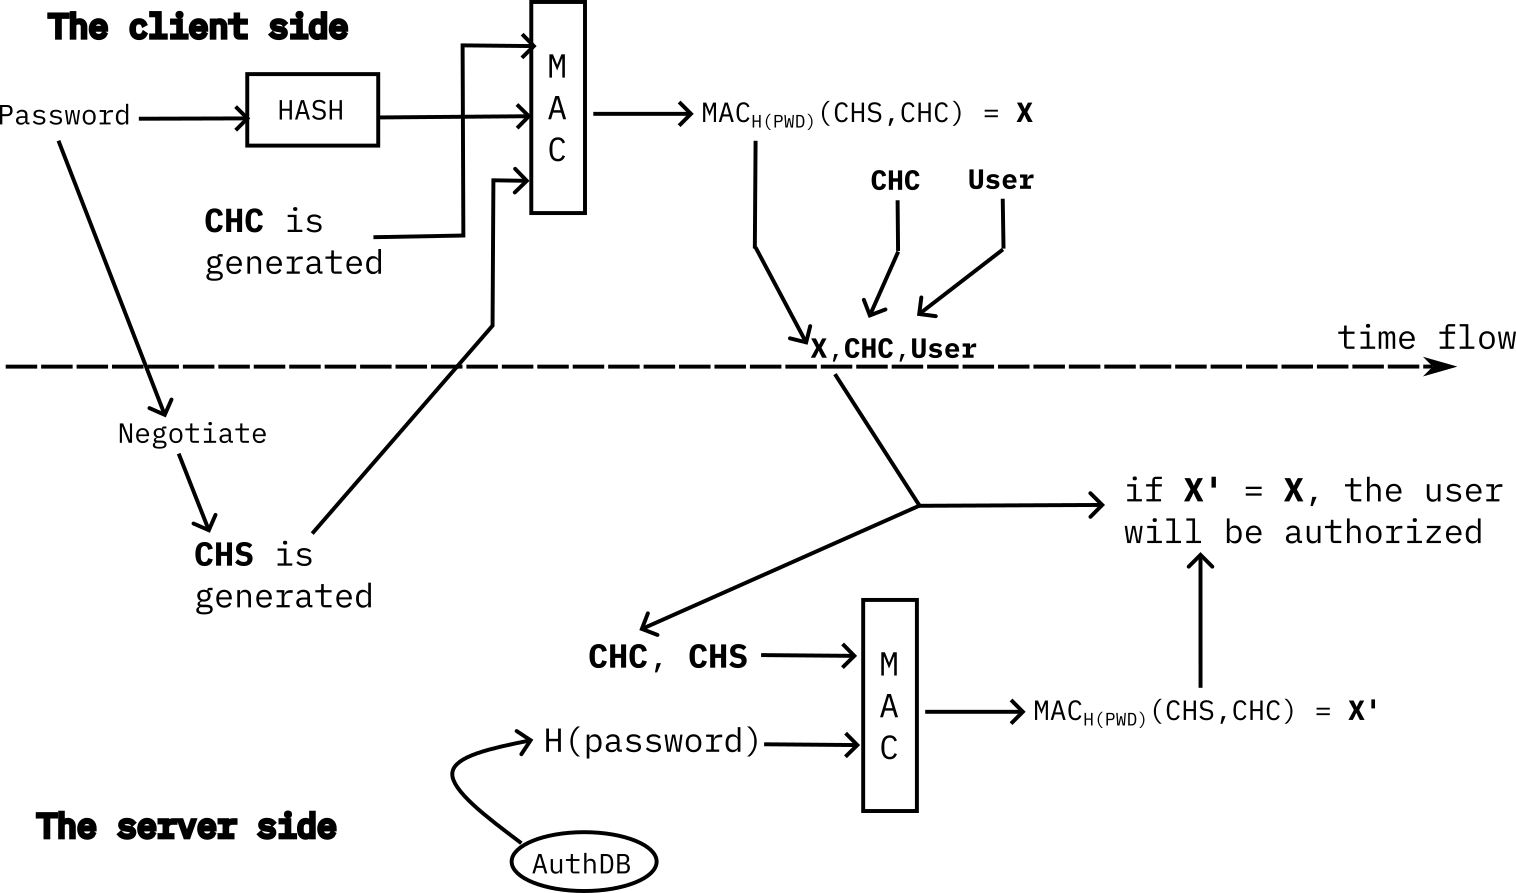
\includegraphics[ width=1.0\linewidth, height=\textheight, keepaspectratio]{./pics/auth/ntlm1.png}
    \caption{The NTLM scheme. A login is first \emph{negotiated} by sending
    username, after which the server sends a \textbf{server challenge}
\texttt{CHS}. Another challenge, the \textbf{client challenge} \texttt{CHC} is
determined and concatenated to the \texttt{CHS} to form a string. The string is
then transformed by a MAC() algorithm by means of the key determined with the
hash of the user's password. MAC\--digest along with username and \texttt{CHC}
are sent back to the server, that is able to check the integrity of the
original message by using the MAC again with the string and with the hash of
the password (present in the AuthDB). The \textbf{only} security control is in
this last phase, where the two strings are checked to be equal.}
    \label{fig:ntlm1}
\end{figure}

A first remark of this NTLM protocol is that \textbf{the server does not prove
its knowledge of the \texttt{H(pwd-user)}} --- in practice, the client
authentication is completely \emph{unilateral} as the server can actually be
impersonated by anyone.

With the established threat model, an attacker can only execute guessing
attacks, as the string \texttt{X} cannot be replayed in future executions
(\texttt{CHS} changes at every execution). The \texttt{H(pwd-user)} is
\textbf{unknown} to the attacker, that only knows the MAC result (\texttt{X}),
\texttt{CHC} and \texttt{CHS}. Equivalently to salted database, an attacker
cannot compute anything in advance --- this means that he must employ a cracking
tool and perform an exaurient search in the password space (or, more cleverly,
adopt a candidate password set as seen in previous chapters).

Unluckily, the encryption algorithm used in NTLM is very \emph{fast} to
compute, all while capturing an NTLM execution is very easy. The consequences
are that guessing attacks are actually possible, and basically
\emph{unavoidable} in Windows environments. The number of realistic guesses is
very high. Windows password have a huge value for attacks, as most
organizations implement \textbf{Single Sign On (SSO)}. Thus, possessing strong
passwords should be a priority in large organizations.

However, on NTLM that is almost \emph{useless}: the client only
\textbf{demonstrates the knowledge of the hash, that is \texttt{H(pwd-user)}}.
Basically, \textbf{knowledge of the hash of a password suffices to impersonate
the user}, a weakness that renders NTLM very dangerous to use. What happens is
that on Windows environments hash knowledge is enough to impersonate an user,
no matter how strong the password is: offline guessing can be done with the
goal of obtaining \texttt{H(pwd-us\-er)} rather than \texttt{pwd-user} itself.
Moreover, softwares capable of extracting the hashes from a Windows machine
exist: when a client is compromised, the user can immediately be impersonated
on the network.

The hash of the password is nowadays computed by a function that is called
\textbf{NetNTLM Hash}: the computation hardness of the function is a lot better
than standard NTLM, however still very weak when compared to blowfish or bcrypt
(53.9k times weaker).

\subsection{NTLM and security guarantees: authentication in practice}

NTLM does not provide \textbf{any security guarantee after authentication}.
Differently from HTTPS (which provides secrecy, integrity and server
authentication), there are no guarantees after a client authenticated to a
server. The drawback of this is that the communication occurs without
encryption or any security guarantee that might be expected from an
authentication protocol (that is, no shared secret key \texttt{K} is
established). Of course, a network attacker can inject application data in open
connections, alter the traffic, and observe everything --- something that cannot
occur in the cases of an authentication procedure that guarantees something
more. Weak protocols in this sense are HTTP BASIC or FORM, POP, and
\textbf{NTLM}. Strong protocols are HTTPS, Personal or Enterprise Wi\--Fi, any
protocol over SSH (secure shell).

MITM attacks are trivial against NTLM. A MITM attacker can simply watch and
collect all material, performing offline guessing on the collected material.
More simply, he can perform a \textbf{relay attack} in which just after he
impersonated the server and the client in a NTLM authentication procedure, he
impersonates the client and further communicates with the server. Of course,
the attacker should be able to impersonate different protocols at once, so that
the attack can work on any service. This all requires the exact timing, and it
only works on a single authentication. Basically, \textbf{NTLM is weak to relay
attacks}.

NTLM can be made much more secure. In fact, NTLM can be upgraded to
\textbf{NTLM with Signing \& Sealing}, in which the server must \emph{prove
knowledge of the hash of the password}, negotiate a secret \texttt{K} with the
client, and after the authentication secrecity, integrity (with the option of
server authentication) are guaranteed. A MITM cannot execute relay attacks
(since he does not know \texttt{K}), however the security mechanism is not
enabled by default.

\section{Kerberos}
\textbf{Kerberos} is a computer-network authentication protocol that
works on the basis of tickets to allow nodes communicating over a non-secure
network to prove their identity to one another in a secure manner. Its
designers aimed it primarily towards a client-server model, and it provides mutual
authentication—both the user and the server verify each other's identity.
Kerberos protocol messages are protected against both eavesdropping and replay
attacks.

Kerberos is built on symmetric-key cryptography and requires a trusted third
party; optionally it might use public-key cryptography during certain phases of
authentication. Kerberos uses \emph{UDP port 88} by default.

Kerberos was initially designed in 1978 by \textbf{Needham} and
\textbf{Schroeder}. In 1981 it had its first attacks, and some fix occurred --
in 1987, the first release called \emph{Project Athena} (MIT), and in 1988 the
first conference took place. Only in \emph{Windows 2000} Microsoft systems
started implementing it for real. History tells that for most crucial protocols
a huge amount of time and money should be spent on research, and the results
can be perceived only after some years.


\subsection{Private Key Cryptography}

In \textbf{private key cryptography}, along with secrecy (encryption) every
message exchange contains a \emph{Message Authentication Code} to provide
\textbf{integrity}. MACs are appended to each message and allow checking for
the integrity of the message. If a receiver realises that the digest of the
message and the MAC don't match, then the message has been subject of errors or it
might have been tampered. For simplicity, MACs will be omitted from now on.

Private key cryptography assures secrecy, mutual authentication and integrity.
It resembles \textbf{digital signature}, since only the real part is able to
use that secure channel (as it owns the specific secret that allow the
communication to take place).

\subsection{A simple version of Kerberos}

The first simplified version of Kerberos has the following properties:
\begin{enumerate}
    \item mutual authentication;
    \item key establishment;
    \item secrecy, integrity, mutual athentication;
    \item uses private key cryptography;
    \item enforces short key lifetimes, with frequent rotation.
\end{enumerate}

The architecture is as follows:
\begin{itemize}
    \item every user \texttt{U} has a \textbf{secret key} \texttt{KU};
    \item every server \texttt{S} has a \textbf{secret key} \texttt{KS};
    \item each secret key had been derived by a \textbf{password}, so that
    \begin{itemize}
        \item \texttt{KU = H(U, pwd-U)};
        \item \texttt{KS = H(S, pwd-S)};
    \end{itemize}
    \item an \textbf{Authentication Server} \texttt{AS} knows all secrets, as it
        possesses an AuthDB containing the pairs \texttt{username, K-username};
    \item the username is used as a \textbf{salt};
    \item every node has a good, local clock.
\end{itemize}

Kerberos is particularly suitable for \textbf{local} environments, as an AS
should exist for all users and servers. This is not scalable, as private key
cryptography can't be managed on a large scale.

The first phase of any login is the \textbf{interactive logon}. An interactive
logon sees a user \emph{locally logging in} a machine (a workstation, a
physical terminal of a server). After the local login, the workstation
immediately authenticates to the AS --- if the operation results successfully,
the interactive logon completes correctly, and the user is correctly
authenticated (he knows \texttt{pwd-U}. The user can use all the services
provided on the local workstation.

The next phase is the \textbf{network logon}. A network logon involves a user's
workstation \texttt{U} authenticating to \textbf{any} server \texttt{S} (he is
authorized to perform the login on). The already\--authenticated workstation
authenticates on user's behalf, and the end result is the user \texttt{U} able
to use services from server \texttt{S}.

In this simplified model, the user workstation \texttt{U} interacts with the authentication server \texttt{AS} by sending a message, containing:
\begin{itemize}
    \item \texttt{U};
    \item \texttt{S} to which a connection should be performed;
    \item \texttt{Eku(t1)}, with \texttt{t1} local clock and \texttt{ku}
        \textbf{private key} known only by the client;
\end{itemize}

If \texttt{t1} is sufficiently close to the clock of \texttt{AS} and the
encryption key is the correct one, then the \texttt{AS} will respond with a
message\footnote{Up to version $4$, \texttt{AS} would respond to messages
\texttt{U,S} without \texttt{Eku(t1)}, thus providing unnecessary material for
offline guessing since an attacker could simply ask for thousands of tickets.},
encrypted with \texttt{ku}, containing the \textbf{session key} \texttt{Kus}
and the clock \texttt{t1}. Since \texttt{ku} had been used, the message is
authentic, and since \texttt{t1} is recent, the message is also fresh. The
session key is a special key constructed by the \texttt{AS} whose purpose is to
allow interaction between \texttt{U} and \texttt{S}.

Since the message is encrypted with \texttt{ku}, how can the server possibly
get \texttt{Kus}? The answer is by means of \textbf{service tickets} --- service
tickets are messages containing \texttt{Kus} encrypted with the key \texttt{ks}
belonging to the server. Service tickets are appended to the response message
to the client. Service ticket is then sent to the server \texttt{S}. A service
ticket contains \texttt{Kus}, can be read only by the server \texttt{S} since
it is encrypted with \texttt{ks}, and can be only issued by \texttt{AS} (since
no other entities will know \texttt{ks}).

A service ticket is of the form \texttt{Eks(Kus, U, S, IP-U, Tas, LIFE, ...)} --
it contains \texttt{Kus}, but also informations regarding the workstation
(user, server, IP of workstation, time of \texttt{AS}, lifetime, and many other
informations) so that the ticket \textbf{can only be used by the legitimate
workstation, to submit requests to the legitimate server}. The lifetime is
provided (usually in minutes) to prevent \emph{replay attacks}.

During a request to \texttt{S}, the workstation \texttt{U} must authenticate as
well, with an \textbf{Authenticator} message encrypted with the session key
\texttt{Kus}. In order to do so, a message \texttt{Ekus(U, IP-U, TU1)} is
appended so that the server can properly read informations on workstation (and
comparing them to common network inspection). If the authentication succeeded,
\texttt{S} will send back to the user \texttt{Ekus(TU1)}, so that he can check
\texttt{S} identity and freshness of communication. Basically, both
authenticator and ticket must agree on user's name, IP address and timestamp
for this to work. The overall scheme is shown in
Figure~\ref{fig:almost-kerberos}.

\begin{figure}[ht]
    \centering
    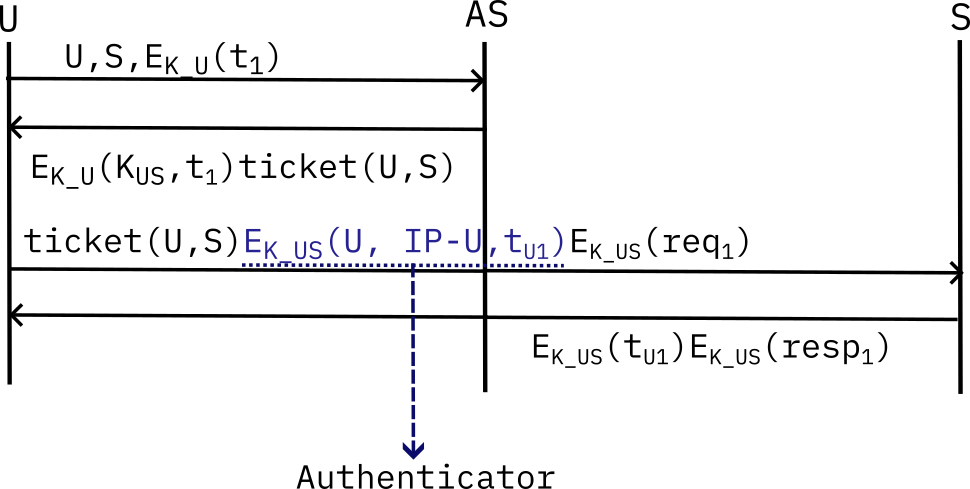
\includegraphics[ width=1.0\linewidth, height=\textheight, keepaspectratio]{./pics/auth/almost-kerberos.png}
    \caption{A simplified overview of the Kerberos protocol.}
    \label{fig:almost-kerberos}
\end{figure}



Network attackers in this path cannot succeed. First of all, communication between
\texttt{U} and \texttt{AS} works perfectly, as the entire process runs on
encrypted communications (by means of secrets known only by the two parties);
secondly, communication between the \texttt{AS} and \texttt{S} guarantees
secrecy, mutual authentication and integrity. The user becomes trusted as long
as it cannot tamper \texttt{Kus}, because it doesn't know \texttt{ks}. An
attacker cannot forge messages that should be encrypted with \texttt{Kus},
cannot impersonate another user (as \texttt{U} would be different). The only
attack left is Denial of Service.

Among a single session (until the ticket expires), all the Kerberos\--related
messages are always the same, as the ticket can be reused again. The only
different things will be timestamps and requests\---responses between
\texttt{U} and \texttt{S}. Since timestamps will mutate, the Authenticator
message will mutate as well.

Kerberos can be seen as a \emph{protocol} for making sure that an
\textbf{Authentication Token}, authentic and intact across untrusted channels,
is presented by its owner and to the legitimate service. With these expedients,
Kerberos is able to provide secrecy, integrity and mutual authentication, at
the cost of a lesser usability, greater costs and greater administration
difficulty.


\subsection{Kerberos and security properties in detail}
\subsubsection{Improving the simplified Kerberos model to withstand replay attacks}

A network attacker cannot read, modify or forge messages; however, he can
\textbf{replay} them:
\begin{itemize}
    \item replaying \emph{responses} will result in a detection, as the
        responses are always matched with the corresponding timestamp;
    \item replaying \emph{requests} will be undetected with the above
        techniques only.
\end{itemize}

However, requests to \texttt{AS} pose no problem, since the attacker will
receive many copies of the same response (containing the service ticket), but
he will never be able to decrypt them --- differently, an attacker may want to
replay some request to a server \texttt{S}, so that \textbf{multiple
executions} of a same command can be provoked.

Since the client will insert the local clock in every sent message, the defense
is to \emph{compare the clock contained in the message with the local clock},
and then \textbf{discard} every message received with \texttt{msg.clock -
rcv.clock} greater than a certain threshold (before of after the
\texttt{rcv.clock}). In other words, \textbf{given a tolerance} $\delta$ every
message whose clock is different from the clock of the receiver will be
discarded. An attacker could still perform a quick replay and send a lot of
requests during the threshold --- this is now possible, however, since
\textbf{the server will store all received message with clock within $\delta$,
and discard all copies of the same message}, thus preventing massive spam of
replay attacks. This technique is also adopted in many modern protocols, such
as \emph{OAuth} and \emph{SPID}.

Kerberos can still be vulnerable to guessing attacks. Guessing can, of course,
only be made against \texttt{Ku} and \texttt{Ks} as both are derived from
password (plus a salt), and not against \texttt{Kus}.

\subsubsection{The three different versions of Kerberos}

Kerberos comes in three versions:
\begin{enumerate}
    \item the \textbf{very strong} configuration, providing \emph{private}
        messages with guarantees of secrecy, integrity and mutual
        authentication;
    \item the \textbf{strong} configuration, providing only \emph{safe}
        messages (integrity and mutual authentication);
    \item the \textbf{so\--so} configuration, in which after the first
        interaction the connection \textbf{is the same as TCP}, therefore it is
        vulnerable to relay attacks just as default NTLM configuration. Sadly,
        this is the default configuration when setting up a Kerberos instance.
\end{enumerate}

The first and strongest configuration is the one we have already seen, and it is depicted in Figure~\ref{fig:very-strong-kerberos}.

\begin{figure}[ht]
    \centering
    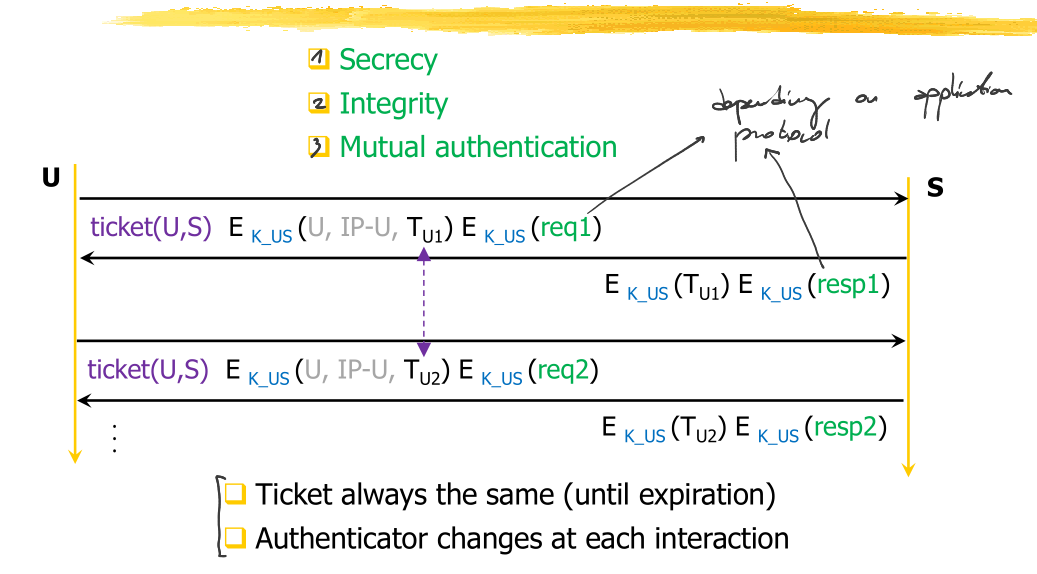
\includegraphics[ width=1.0\linewidth, height=\textheight, keepaspectratio]{./pics/auth/very-strong-kerberos.png}
    \caption{The ``very strong'' Kerberos configuration.}
    \label{fig:very-strong-kerberos}
\end{figure}

The second configuration has \textbf{no secrecy in requests}, only providing
mutual authentication and integrity by means of \emph{Message Authentication
Codes} appended in each message (Figure~\ref{fig:strong-kerberos}).

\begin{figure}[ht]
    \centering
    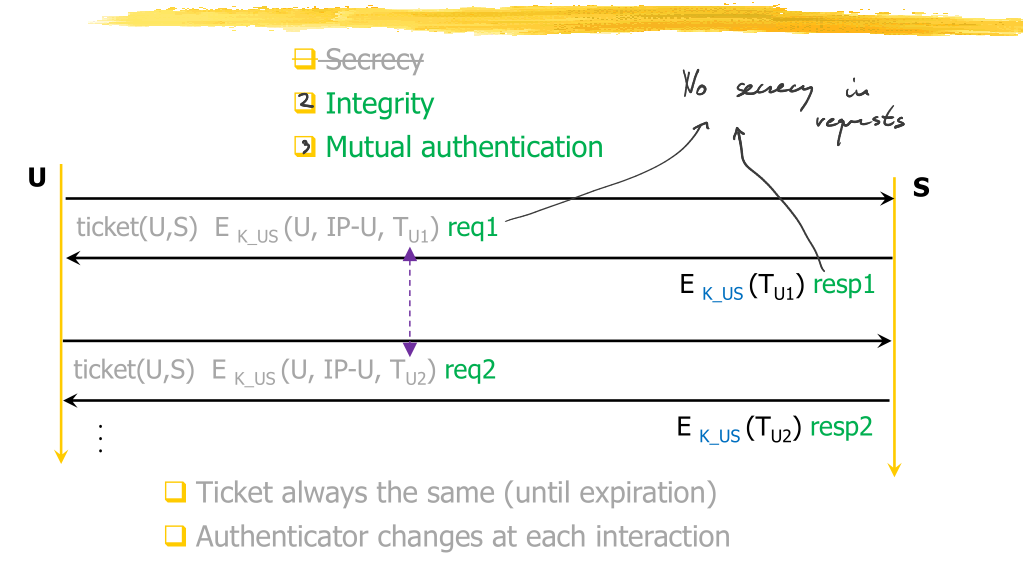
\includegraphics[ width=1.0\linewidth, height=\textheight, keepaspectratio]{./pics/auth/strong-kerberos.png}
    \caption{The ``strong'' Kerberos configuration.}
    \label{fig:strong-kerberos}
\end{figure}

The third, the weakest of all, provides mutual authentication \textbf{only} in
the first interaction of the protocol (Figure~\ref{fig:so-so-kerberos}).

\begin{figure}[ht]
    \centering
    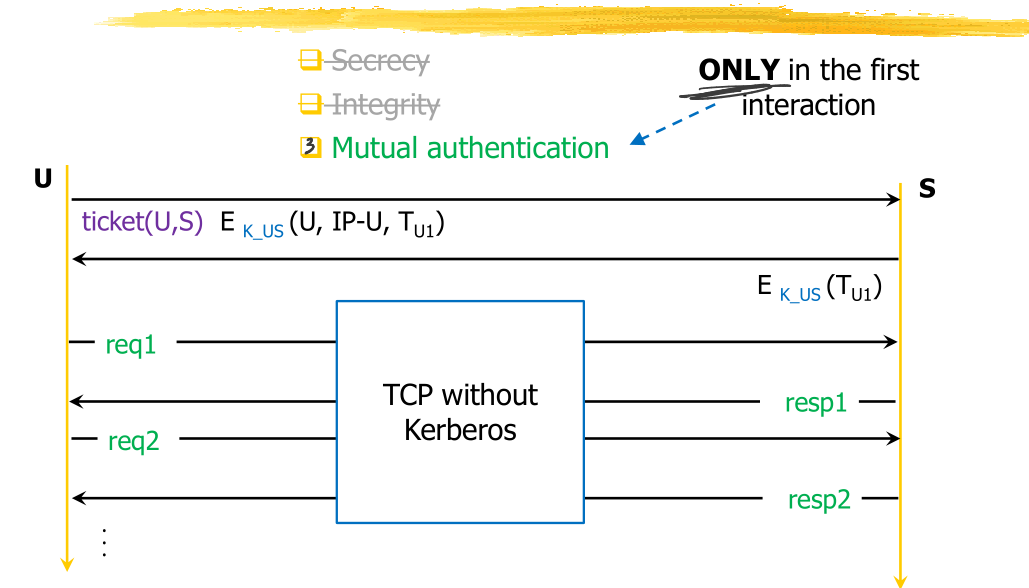
\includegraphics[ width=1.0\linewidth, height=\textheight, keepaspectratio]{./pics/auth/so-so-kerberos.png}
    \caption{The ``so-so'' Kerberos configuration.}
    \label{fig:so-so-kerberos}
\end{figure}

\subsubsection{Ticket lifetime}

During a \textbf{Kerberos Session} there exists a single ticket. After the
ticket expires, a new Kerberos Session should be created and a new ticket
should be granted, all by contacting the \texttt{AS} again. The Kerberos
Session and the ticket lifetime is \emph{completely independent} of the TCP
connection lifetime --- a single TCP connection can end up by using
\emph{multiple} service tickets, and a single service ticket can be used on
\emph{multiple} TCP connections.

The main reason to adopt a limited lifetime is the \emph{Crypto Prudent
Engineering Practice}, which states that \textbf{every key must be changed
every now and then}, a fundamental practice for every practical application in
cryptography. There could be many reasons for this, for instance the
cryptographic algorithm could have weaknesses exploitable by collecting a lot
of traffic, or the key might be found \emph{somehow}, so all the traffic would
be decrypted, forever. Thus, the session key that the service ticket grants
must be changed every now and then.

The problem with ticket expiring is that it protects a strong key by increasing
the risk on a \textbf{weaker} key (\texttt{Ku}), by providing more
opportunities for observing traffic (dictionary attack), and more traffic for
cryptanalysis. The issue is solved by means of KDC (next section).

\subsection{Key Distribution Center}

In order to understand how the real Kerberos works, further modifications
should be done.

The \textbf{Key Distribution Center} is a server belonging to a Kerberos instance
whose goal is to \textbf{provide tickets}. A real Kerberos works with two,
distinct services (can be run on the same machine --- in fact, it runs on port
88 on the same machine): one that \textbf{initiates authentication}, and the
other one that \textbf{provides tickets}. The first one is the \texttt{AS} that
had already been depicted in the previous paragraphs, while the KDC role will
be explained now.

Suppose a user wants a ticket to communicate with a server \texttt{S}. The user
sends a request to the \textbf{Ticket Granting Service} (\texttt{TGS}). The
\texttt{AS} grants the user a \textbf{Ticket Granting Ticket} (TGT), that is a
ticket with which the user workstation will be able to communicate with the
\texttt{TGS}. After that, the user presents its \texttt{TGT} to the
\texttt{TGS}, along with a request for service \texttt{S}. The \texttt{TGS}
will respond with the \textbf{service ticket} for communucating with service
\texttt{S}. To summarise, a first ticket --- the \emph{Ticket Granting Ticket} --- should be provided by the Ticket Granting Service to request other tickets. Subsequent tickets --- the \emph{Service Tickets} --- are the same ones we illustrated in the previous sections. Next
Figures~\ref{fig:real-kerberos-1}~and~\ref{fig:real-kerberos-2} illustrate the
entire process in detail.

\begin{figure}[ht]
    \centering
    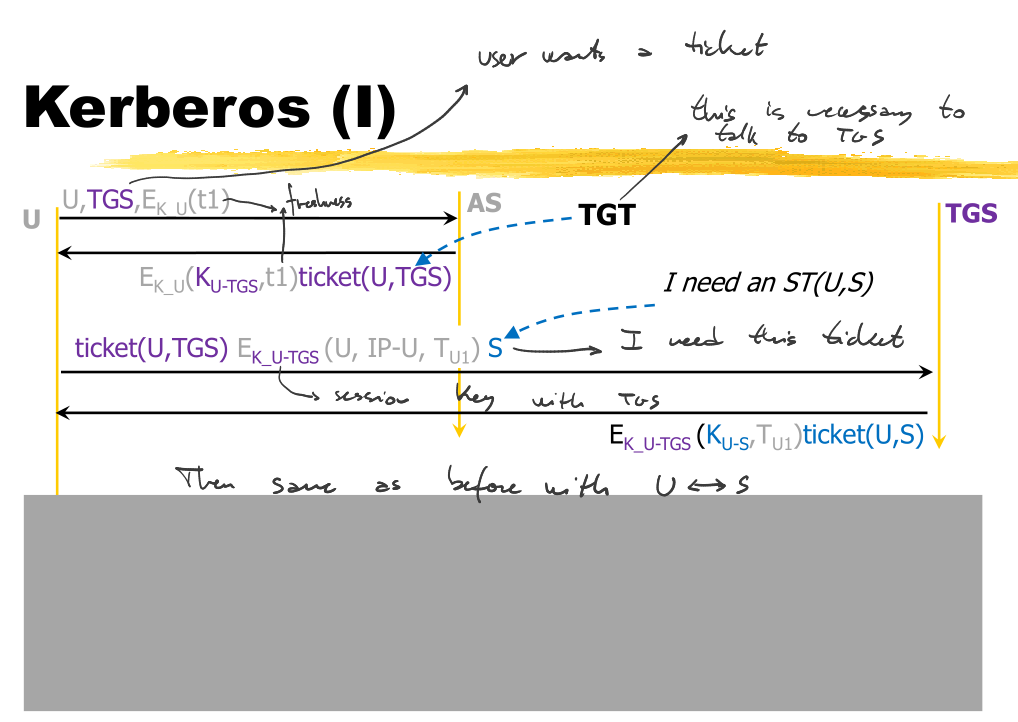
\includegraphics[ width=1.0\linewidth, height=\textheight, keepaspectratio]{./pics/auth/real-kerberos-1.png}
    \caption{The first steps of real Kerberos.}
    \label{fig:real-kerberos-1}
\end{figure}

\begin{figure}[ht]
    \centering
    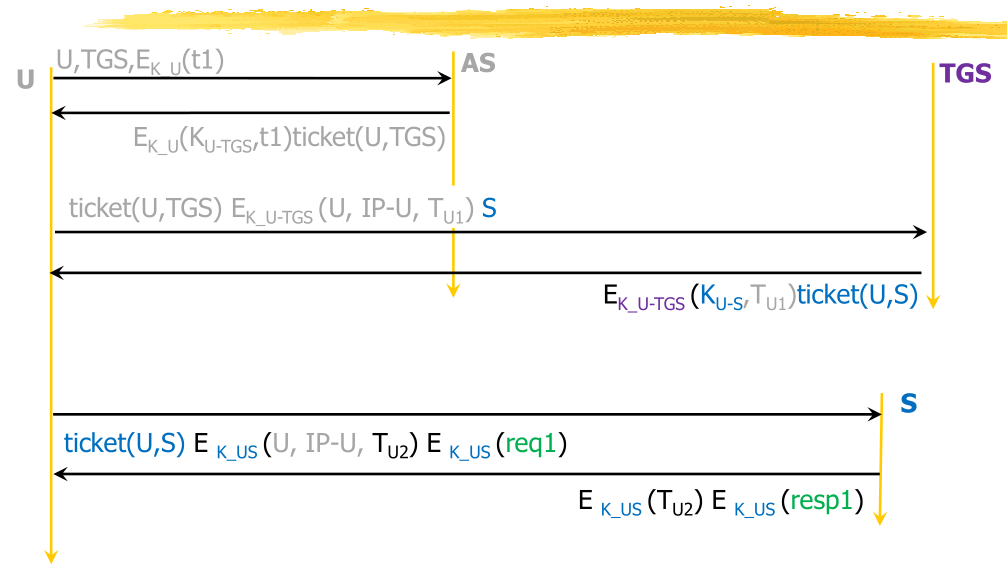
\includegraphics[ width=1.0\linewidth, height=\textheight, keepaspectratio]{./pics/auth/real-kerberos-2.png}
    \caption{The further steps of real Kerberos.}
    \label{fig:real-kerberos-2}
\end{figure}


\clearpage


Hence, the process can be summarized in $4$, distinct steps (two phases):
\begin{enumerate}
    \item the user \texttt{U} performs an \textbf{interactive logon} on the
        workstation. A concatenation of username and password is passwd through
        a hash function, which produces \texttt{Ku};
    \item the workstation \emph{proves its knowledge of \texttt{Ku}} with the
        Authentication Server \texttt{AS} --- the latter grants the user's
        workstation a \textbf{ticket granting ticket}, along with session key
        \texttt{Ku-tgs}. The \emph{interactive logon} phase ends here;
    \item the user performs a \textbf{network logon} to a service \texttt{S}.
        The workstation presents the TGT to the \texttt{TGS}, also proving the
        knowledge of \texttt{Ku-tgs}; the \texttt{TGS} gives it the
        \emph{session ticket} for the communication between \texttt{U} and
        \texttt{S}, along with \texttt{Ku-s};
    \item the user completes the network logon by presenting the ticket to
        \texttt{S}, proving knowledge of \texttt{Ku-s}.
\end{enumerate}

A Ticket Granting Ticket lasts \emph{hours}, and can be used to request new
service tickets until it expires. During a single day, some of them might be
requested by a workstation whose TGTs expired. A service ticket, instead, lasts
\emph{minutes}. This means that \emph{the secret \texttt{Ku} is used only once
in hours}, protecting it from the collection of guessing material, while the
strong secret (the session key) is rotated multiple times, possibly hundreds of
times each day. Basically, the high volume traffic is only performed with
strong secrets, protecting the weaker user key.

Some weak points of real Kerberos exist. For instance,
\begin{itemize}
    \item collecting service tickets is very easy. Service tickets are
        encrypted with \texttt{Ks}, hence collecting guessing material to
        attack server password is a realistic threat;
    \item if weak or default passwords are used this is dangerous;
    \item even more dangerous in the case of \emph{overprivilege}.
\end{itemize}
hence, an attacker that has obtained credentials of a single user (very
realistic) can then obtain ST(S) for \textbf{any} server \texttt{S} by simply
asking \texttt{TGS} for tickets (for this reason, servers passwords must be
managed \textbf{very} carefully); this attack is known as
\textbf{Kerberoasting}. There are many automated tools for this data
collection, and there is no need to observe the traffic (only by communicating
and possessing credentials of a user). When the attacker can only observe (and
does not possess credentials) the attack is feasible, but not easy. In fact, he
must perform the equivalent of an offline guessing attack, with salted
passwords. This is still feasible as \texttt{Kerberos 5} protocol allows
computing 13200 times more hashes than \texttt{bcrypt} or \texttt{blowfish}.

\section{Access Management in Kerberos}

Kerberos allows fine\--tuning the \textbf{permissions} related to
\textbf{Access Management}. In particular, access management is performed in a
\emph{centralized fashion}, with \textbf{access right specified on the ticket}.
Basically, when a ticket is forged by a \texttt{TGS}, the access rights for a
user are defined in the ticket (the server trusts them blindly) since the
access rights are set up in the KDC. User requesting an operation which is out
of his rights will result in a ``not authorized'' message from the server. Each
resource has an Access Control List described in terms of groups of usernames
-- the ticket specifies which groups the username belongs to.

Kerberos can only work effectively towards a \emph{single organization}. In fact:
\begin{itemize}
    \item a server in the second organization must be able to verify the
        authenticity and the integrity of tokens \textbf{issued by the first
        organization};
    \item the protocol is not NAT\--friendly;
    \item the access right policies should be mapped between organizations
        (hard to do due to privacy);
    \item each organization should trust the other. Perhaps, this is the most
        crucial aspect.
\end{itemize}

For the above reasons, Kerberos is practically used only between different
parts of a same organization --- and not across the internetwork. Protocols that
reliably work across the internet are \textbf{SAML}, which supports
authentication and authorization, often used for authentication only, as in the
case of SPID --- and \textbf{OAuth}, which supports authentication and
authorization as well.






\chapter{Identity and Access Management}

Large organizations involve hundreds of servers, each one storing files and
databases, thousands of workstations (either private or shared) and thousands
of users (belonging to tens of partially\--overlapping groups). Some servers
might even be accessible from the outside (POP, HTTP, for example). Users and
groups are said to be \textbf{identities}, while everything else falls in the
category of \textbf{resources}. What an identity \texttt{U} can do, is to
request \textbf{operation} \texttt{O} on resource \texttt{R}. 

Every software that manages a resource authenticats the identity that requests
an operation, and verifies whether that identity has the access rights (the
authorization) for such operation. That should be done in a centralized
fashion, with a single \texttt{AuthDB} managin all identities and related
permissions.

The \textbf{Identity and Access Management} are the \emph{procedures} and
\emph{technologies} for management of individual \emph{identities}, their
\emph{authentication}, \emph{authorization}, \emph{roles} and ultimately their
\emph{access rights} \textbf{within} or \textbf{across} system and enterprise
boundaries.

Almost all large organizations use \textbf{Windows Active Directory}, along
with \textbf{LDAP}.

\section{Identity and Access Management within an Organization}

IAM within an organizations is realized thanks to the \textbf{Directory
Service}. A Directory Service is a \emph{centralized} repository containing all
\emph{identities} and their \emph{credentials}, all \emph{resources} and all
\emph{access rights} associations between identities and resources.

A process of \emph{Single Sign On} can be performed by users, with each
resource executing authentication by interacting with \texttt{DS}. Access
rights are stored on \texttt{DS} --- therefore, authorization can be queried to
the Directory Service.

\subsection{Windows Active Directory}

On \textbf{Windows Active Directory}, a single entity --- the \textbf{Domain
Controller} --- runs the three single most important services:
\begin{itemize}
    \item the \emph{Kerberos AS};
    \item the \emph{Kerberos TGS};
    \item the \emph{Directory Service};
\end{itemize}
thus, it runs both Kerberos and the Directory Serivce and should definitely be
safeguarded from attackers. Obtaining access to this server usually leads to a
complete catastrophe.

Active Directory works wonderfully over Kerberos. The process is the following
one:
\begin{enumerate}
    \item \texttt{U} presents credentials to a workstation and performs the
        first phase of interactive logon;
    \item the workstation obtains \texttt{TGT(U)} from \texttt{DC};
    \item the workstation \emph{verifies} whether \texttt{TGT(U)} specifies
        that \emph{the user \texttt{U} can logon on the workstation};
    \item if yes, the workstation stores \texttt{TGT(U)} in its memory;
    \item the network logon phase starts. The workstation presents
        \texttt{TGT(U)} to the Domain Controller, which in return grants
        \texttt{ST(U,S)};
    \item the workstation presents \texttt{ST(U,S)} to server \texttt{S};
    \item the server \texttt{S} verifies in \texttt{ST(U,S)} \emph{which
        operations} the user \texttt{U} can execute on \texttt{S};
    \item the user has correct privileges, both workstation and server
        \texttt{S} store \texttt{ST(U,S)} in their memory;
    \item the server executes \texttt{S}.
\end{enumerate}

A third way to logon is the \textbf{Remote Logon}. A remote logon occurs when a
user wants to connect to a different workstation (not the same one) --- it works
like in the case of a server:
\begin{enumerate}
    \item the workstation presents \texttt{TGT(U)} to \texttt{DC} and obtains
        \texttt{ST(U,WKS')};
    \item the workstation presents \texttt{ST(U,WKS')} to \texttt{WKS'};
    \item the remote workstation \texttt{WKS'} \emph{verifies} in
        \texttt{ST(U,WKS')} which operations \emph{the user \texttt{U} can
        execute on \texttt{WKS'}}.
    \item if all correct, the workstation and the remote workstation will store
        \texttt{ST(U,WKS')} on their memory.
\end{enumerate}

A fourth way of logon is the \textbf{Network Logon with Delegation}. In this
scenario, an user \texttt{U} authenticates to \texttt{S}, and the latter
accesses \texttt{S'} \textbf{on behalf of \texttt{U}}. The typical case is when
the \texttt{S} is a web server, and \texttt{S'} is a database server. In this
case,
\begin{enumerate}
    \item the ticket \texttt{ST(U,S)} must be a \textbf{delegation ticket},
        having a special flag denoting such peculiarity;
    \item the server \texttt{S} presents \texttt{ST(U,S)} to \texttt{DC},
        obtaining \texttt{ST(U,S')} --- with this ticket, the server \texttt{S'}
        obtains the user's identity;
    \item both servers keep \texttt{ST(U,S')} in memory.
\end{enumerate}


An important remark is that \emph{everything can be done with NTLM as well},
for compatibiluty reasons. The important aspect is that \textbf{credentials
such as hashes of user passwords are stored in memory}, always present in
workstations --- a network attacker can grab oggline guessing material for
\texttt{H(pwd-U)}, a secret that it allows impersonating the user \texttt{U}.

\subsection{LDAP}

\textbf{Lightweight Directory Access Protocol} is a protocol designed for Linux
(or different than Windows) machines to interact with an exiting Active
Directory configuration.

Some services or web applications run on Linux. In order to interact with users
of an existing Active Directory configuration, the Linux machine \textbf{asks
Directory Service by means of the dedicated LDAP application protocol} if the
credentials are valid and what are the proper access rights of an user (logged
in with an application\--specific authentication protocol, let's say HTTPS,
FTP, POP and so on). Basically, the Linux machines authenticates to the
\texttt{DC} with an \emph{LDAP Authentication}, for instance with
\emph{TLS+username\--password} (\textbf{LDAPS}) carried on a special LDAP
message. Certain LDAP operations require \textbf{LDAP authentication} of the
client application. After that, the Linux machine is successfully authenticated
to the \texttt{DC}, and can then ask for credentials validity or access rights.


LDAP has a double meaning:
\begin{enumerate}
    \item a \textbf{standard} for describing entities of IT interest, such as
        \emph{users}, \emph{resources} and \emph{access rights};
    \item a \textbf{protocol} for querying a directory service (the server that
        stores those descriptions).
\end{enumerate}





\part{Cyberattacks}

\chapter{An introduction to Vulnerabilities}

\textbf{Vulnerabilities} are a \textbf{mistake in software} that can be
directly used to \emph{gain access} to a system or to a network.

The list of known vulnerabilities (CVE, \emph{Common Vulnerabilities and
Exposures}) can be found at \texttt{https://cve.mitre.org/}.

Vulnerabilities allow a wide range of attacks to succeed, with impacts ranging
from better to worse:
\begin{enumerate}
    \item information disclosure;
    \item privilege escalation;
    \item code execution of existing operations, or arbitrary code execution.
\end{enumerate}

and are also categorized according to various methods of execution (not
exhaustive list):
\begin{itemize}
    \item physical access needed;
    \item can be exploited by a malicious running program;
    \item remote execution with human interaction;
    \item remote execution without human interaction.
\end{itemize}



A more general definition is the following one:

\vspace*{1cm}
\begin{center}
    \emph{``A vulnerability is a flaw or weakness in a computer system, in its
    security procedures or internal controls, which could be exploited to
violate the system security policy. (NIST SP 800-28 Version 2)''}
\end{center}
\vspace*{1cm}

Typical examples of vulnerabilities are:
\begin{itemize}
    \item over\--privileged user accounts;
    \item oversized administrator groups;
    \item bad practice in workstation administration;
    \item bad practice in password management;
    \item excessively loose firewall policies;
    \item and so on\dots
\end{itemize}

In a nutshell, vulnerabilities are software or configuration\---procedural
\textbf{mistakes} that allow an attacker to violate the security policies in
effect.

Vulnerabilities are a \emph{growing trend} (we are not in the range of
20000\--per\--year), and they are only the publicly known vulnerabilities.
There are, however, the so\--called \textbf{zero\--day} vulnerabilities which
are known to the attacker only, and unknown to both software manufacturer and
defender.

\textbf{Every kind of software} can be affected by vulnerabilities.
Vulnerabilities are an intrinsic feature of software --- not a sporadic,
occasional phenomenon. In practice, those categories can be affected:
\begin{itemize}
    \item end user software;
    \item network devices;
    \item security software;
    \item software implementing security protocols;
    \item Industrial Control Systems (ICS);
    \item Medical Devices;
    \item IoT devices (Cars, Ships, home devices);
    \item and so on\dots
\end{itemize}


\section{The Common Vulnerability Enumeration procedure}

The \textbf{Common Vulnerability Enumeration} is a procedure for assigning a
\emph{unique ID} to every known vulnerability. The first step is the
\emph{submission} of the vulnerability details to a certain consortium (for
instance, \texttt{https://\-www\-.cve.org}; \emph{analysis} will follow by
\begin{itemize}
    \item assignment of a new ID for the vulnerability, in format
        \texttt{CVE-YYYY-NNNN}\dots;
    \item merging of the vulnerability with an existing one, if already
        existing.
\end{itemize}

CVE is the standard de facto nowadays, and all the organizations and documents
will refer to a certain vulnerability by the same ID, its CVE. This is of a
huge importance in order to avoid any confusion.

Along with the CVE, the \textbf{impact} (or \textbf{risk evaluation}) of a
vulnerability is provided, so that a defender can understand the danger of the
vulnerability in question. Moreover, \textbf{reason} can be provided as well
(does the attacker induce a crash? does the attacker induce an endless loop?
does the device has a too small amount of resources? can the attacker consume
all resources easily?)

Parallel to CVEs, there exist \textbf{Common Weakness Enumeration} (CWE). CWEs
are a \emph{list of types of mistakes}, constructed \emph{once and for all}
(periodically revisited). Some of these mistakes in the list include
\begin{itemize}
    \item weak encryption;
    \item improper validation of syntactic correctness in input;
    \item improper certificate validation;
    \item improper access control;
    \item improper\dots
\end{itemize}

Each CVE might be associated with one or more \textbf{CWE}; this is very useful
in order to grasp the underlying reasons quickly.





\chapter{Attacks}

\section{The reasons behind attacks}

Attacks are most frequently done to \textbf{obtain money}. The first and
foremost reason will always be to make money as easiest as possible. Some
attackers, however, might be motivated enough to performing an attack to
\textbf{steal informations} or \textbf{distrupting the operations} of a
target organization.

Attacks are a \textbf{professional activity}, with criminal groups of tens of
people, hierarchically structured, and teams that are able to update malwares
(for instance, the Conti Group updated their malwares every 4 hours, in order
to avoid detection from \emph{Windows Defender}, so that signature is
different). To obtain money, many creative ways do exist:
\begin{itemize}
    \item steal and use \emph{banking credentials};
    \item steal and sell \emph{credentials};
    \item steal and sell \emph{long term cookies};
    \item employ \emph{Remote Access Trojans} to infect a device, and sell or
        rent it;
    \item and so on.
\end{itemize}

Usually, the victim is \textbf{not} aware of what happened, except in the case
of \textbf{ransomwares} in which the victim is asked to pay an amount of money
in order to unlock the files on his computer that had been encrypted by the
attacker. Another kind of malware \emph{steals} data instead of encrypting it,
asking ransom for not making it public.

With all the above attacks, \emph{the attack cost is very low}, while the
\emph{potential Return on Investment (ROI) is very high)}: this means that a
lot of potential attackers are incentivized to perform attacks to obtain money.
On top of this, anonymous payments worldwide allowed attackers to ask for
ransoms anonimously, while the importance of data for organizations has grown
exponentially in the last years. Ultimately, this is a huge societal problem.

Three distinct target categories might exist:
\begin{itemize}
    \item organizations --- servers and data;
    \item Industrial Control Systems --- sensors and actuators;
    \item single individuals;
\end{itemize}

each one possessing their own attackers and their own crucial aspects.

The term Organizations covers a whole range of entities, such as Hospitals,
administration of manufacturing companies, universities, and any other entity
that possesses servers and owns data. An organization might or might not
possess an ICS infrastructure --- thus, with organization we mean the
administration, logistics, payroll, sales\---purchasing, warehouse,
email\---web (and so on) part, while with ICS one explicitly suggests the
sensors and actuators infrastructure in a manufacturing or control process.

Organizations are often under attack of criminal groups. Criminal groups
usually possess high skill and a great amount of resources, that very often
exceeds those of the target organizations. Crime groups will typically attack
organizations in order to get huge amounts of money with the least possible
effort --- a rational behavior.

A lot of money can be obtained by attacking
\begin{itemize}
    \item single organizations --- asking for huge ransoms;
    \item many individuals --- asking for small ransoms;
\end{itemize}

while attacks on ICSs are frequently justified by other motivations (for
instance, disruption and information disclosure). In fact, attacks to ICS
rarely grant money. Very often, attacks to single individuals are designed to
affect a very broad range of devices, to maximize the possible targets. Each
individual will likely yield a small amount of money, but the very wide set of
victims will provide a large amount of money, enough to justify the efforts.
Ultimately, attacking a category of devices is far simpler than attacking
powerful organizations.






\section{Attacking an organization}

Attacking an organizations usually is a many\--steps process: several phases
follow one after the other, each of several steps, that can last from minutes
to months. To describe attack phases, several \emph{models} have been built;
the most famous two are the \textbf{Kill chain} model, the first widely used,
and the \textbf{MITRE ATT\&CK} model, the one that represents today's standard.

The MITRE ATT\&CK framework is used to describe an attack, and is composed of
13 possible phases, called \emph{Tactics} --- some tactics are optional for an
attacker, so that an attack can succeed without seeing all of the tactics
involved. Tactics are also not necessarily executed in sequence.

Each tactic comprises several \emph{Techniques}, that are the ways for
executing each step of a tactic.

The MITRE ATT\&CK framework involves three \emph{Matrices} in which all the
tactics and techniques are
exposed\footnote{https://attack.mitre.org/matrices/enterprise/}.

The role of vulnerabilities is relevant in all tactics that involves
penetrating security breaches; that are \emph{Initial Access},
\emph{Execution}, \emph{Lateral Movement} and \emph{Privilege Escalation}.

\subsection{Initial Access}

The \textbf{Initial Access} tactic is the one that is almost always observed:
an attacker overcomes the first defenses of an organization. Several techniques
exist:
\begin{description}
    \item[Drive\--by Compromise] A user visits a website over the normal course
        of browsing, and a \emph{vulnerability} is exploited
    \item[Exploit Public\--Facing Application] A \emph{vulnerability
        exploitation} is performed against an internet\--facing machine (be it
        a server or a workstation)
    \item[Phishing] \emph{Malicious attachments} or links in e\--mails lead to a
        vulnerability exploitation
    \item[Valid Accounts] \emph{Compromised credentials} are used to enter the organization
    \item[Other 5 techniques] in MITRE ATT\&CK framework
\end{description}

A remark is that the techniques either exploit an existing vulnerability or get
to deceipt a real human.

An important cornerstone of initial access is \textbf{phishing}. Phishing is a still widely used and very effective attack technique, which is of two forms,
\begin{itemize}
    \item \textbf{non\--targeted}, when adversaries conduct malware spam
        campaigns or other non\--targeted phishing attempts, with even low
        success rates leading to huge gains (cost\--effective);
    \item \textbf{targeted}, in the case of \textbf{spearphishing}: a specific
        individual, company or industry is object of targeting by the
        adversary. Defending against spearphishing is \textbf{very difficult},
        and it usually follows the phase of \emph{Reconnaissance}.
\end{itemize}


\subsection{Execution}

\textbf{Execution} techniques result in an \emph{adversary\--controlled} code,
running within the organizations. Twelve techniques exist for this. Attacker's
code is usually arbitrary code, in the sense that the device is now completely
controlled by the attacker and can respond at will.

\subsection{Persistence}

\textbf{Persistence} should be granted across \emph{system restarts},
\emph{changed credentials} and \emph{interruptions} that could cut off the
attacker's access. Nineteen techniques exist. Persistence is necessary in order
to keep the infected machines as such --- attacks might require weeks of
efforts, so an attacker should carefully design its exploits so that they will
also grant persistence across interuptions or configuration changes.

\subsection{Establishing Command \& Control}

\textbf{Command \& Control} are a set of techniques that adversaries may use
to \emph{communicate with systems under their control}, within a victim
network. Adversaries commonly attempt to \emph{mimick normal, expected traffic
to avoid detection} --- usually by means of existing protocols, but new
``unseen'' protocols might be created by an attacker. The attacker will also
\emph{obfuscate his location} to avoid detection from the defenders or other
security organizations.

An example of C\&C structure is the \textbf{DNS Tunneling} technique, in which
an attacker controlled device encodes a \emph{request message} to attacker in a
DNS query, for instance \texttt{dfg99872gh\-.innocent.com A?} --- whose CNAME
response will be let's say \texttt{hhjsd67\-.innocent.com}, encoding a response
message from the attacker. This way, a very hard to detect channel can be
established. Sixteen more techniques exist.

\subsection{Discovery}

\textbf{Discovery} are a set of techniques in which an attacker \emph{gains
knowledge} about the internal environment of an organizations and decides how
to act accordingly. The goal of discovery is to learn of networks, hosts, devices,
applications, but also users, groups, access rights. Twentynine techniques
exist.

A simple and lightweight program for discovery is \textbf{\texttt{nmap}}
(Network Mapper), an open source tool for \emph{network exploration} and
\emph{security auditing}. The tool \texttt{nmap} is capable to scan either
large networks or single hosts --- it uses raw IP packets in novel ways, to
determine:
\begin{itemize}
    \item what \emph{hosts} are available on the network;
    \item the \emph{services} that are running;
    \item the \emph{Operating Systems} and their version the hosts are running;
    \item the kind of \emph{firewalls} in use;
    \item and many more.
\end{itemize}

Usually, \texttt{nmap} is quite noisy, but with certain flags it can be
configured to be hardly detectable. Of course, many more programs exist for
this purpose.


\subsection{Lateral movement}

\textbf{Lateral movement} is the phase in which an attacker, after having
obtained access to a single point internal to the organization, performs
attacks and operation in which tries to access new devices, usually in the same
privilege sphere that the already attacked device lies; applying then Execution
and Persistence on other hosts. Lateral movement, indeed, is much easier when
the attacker had obtained the privileges of an administrator. There are 9
techniques for lateral movement in MITRE ATT\&CK framework, under the tactic
\emph{Lateral Movement}.

Usually, the lateral movement phase comes after the attacker gained foothold
during the first phase and after having guaranteed \textbf{persistence} with
related techniques.

Lateral movement abuse is based on expansion of \emph{credentials} and
\emph{access rights}, executed with \emph{credentials misuse},
\emph{vulnerability exploitation} and \emph{Access Rights abuse}. Usually, a
crucial aspect allowing all of this is \textbf{misconfiguration}, with
overprivilege or inadequate account auditing. An attacker might be able to
devise a technique to circumvent access right policies, by exploiting bad
configurations from careless system administrators.

With lateral movement, an attacker can access various kind of data --- which and
with which access rights will depend on the available credentials. Of course,
if the Domain Controller is accessed, the attacker will have the upper hand on
the defenders, basically owning the data across the entire section of the organization pertaining to the Domain Controller.

The main reasons for success of lateral movement are the following ones:
\begin{itemize}
    \item target has some device with \emph{default} credentials;
    \item target has some device with \emph{easy to guess} credentials;
    \item target has some device accessible by \emph{stuffing or spraying} credentials;
    \item credentials used locally by the attacker have some \emph{access
        rights} on the target --- suppose the attacker managed to get his hands
        on a privileged machine: the remote logon, for instance, will grant him
        high access rights;
    \item an unpatched \emph{vulnerability} can be exploited;
    \item a careless system administrator did a poor job regarding access
        rights, misconfiguring them;
    \item and so on\dots
\end{itemize}

For instance, the tool \texttt{CrackMapExec} is able to \emph{identify} all
machines in the provided IP range, \emph{attempt credentials} on those machines
and ultimately \emph{extract password hashes} from all machines, where local
admin.

Lateral movement might happend with automated tools as well. The automated tool
will attempt logon on more and more machines, making \emph{credential set}
progressively larger and larger, until some credential allows executing
operations for exfiltration\--impact. This can be done either with
Kerberoasting or NetNTLM Collection.


\subsection{Exfiltration}

The end goal of \textbf{Exfiltration} is to \textbf{steal data} from the target
machines --- transferring it over the already set up C\&C channel (or an
alternate channel), usually employing compression, encryption and paying
attention to size limits. There are 9 techniques to do so.

For instance, \texttt{HTran} is a tool for \emph{proxying TCP connections} --
installed on unsuspecting machines with prior attacks, it opens a TCP
connection to a proxy, while the latter opens a connection to the attacker. Of
course, many instances of \texttt{HTran} could be running between the attacker
and the organization. It makes harder for the defender to guess where the
attacker is. \texttt{HTran} usually hides its traffic on the majority of HTTPS
users in the organizations, thus with the traffic commonly leaving the
organizations without raising suspects. 

Exfiltration effort might be split between many devices that are
infected, in order to both relieve the load across devices and to make harder
to detect the illicit traffic.

\subsection{Reconnaissance}

In this phase, the adversary is trying to gather information they can use to
plan future operations towards a target, before attack.

\textbf{Reconnaissance} consists of techniques that involve adversaries
actively or passively gathering information that can be used to support
targeting. Such information may include details of the victim organization,
infrastructure, or staff/personnel. This information can be leveraged by the
adversary to aid in other phases of the adversary lifecycle, such as using
gathered information to plan and execute Initial Access, to scope and
prioritize post-compromise objectives, or to drive and lead further
Reconnaissance efforts. This is done \emph{before} attacking.

There are 10 techniques.

\subsection{Resource Development}

The adversary is trying to establish resources they can use to support
operations towards a target, before the attack occurs.

\textbf{Resource Development} consists of techniques that involve adversaries
creating, purchasing, or compromising/stealing resources that can be used to
support targeting. Such resources include infrastructure, accounts, or
capabilities. These resources can be leveraged by the adversary to aid in other
phases of the adversary lifecycle, such as using purchased domains to support
Command and Control, email accounts for phishing as a part of Initial Access,
or stealing code signing certificates to help with Defense Evasion. This is
done \emph{prior} to executing the attack, and consists in 7 different
techniques.

\subsection{Impact}

The adversary is trying to manipulate, interrupt, or destroy your systems and
data. This is done \emph{in place} of \emph{Exfiltration} --- for an attacker,
it might suffice to interrupt data services at organization (disruption).

\textbf{Impact} consists of techniques that adversaries use to disrupt
availability or compromise integrity by manipulating business and operational
processes. Techniques used for impact can include destroying or tampering with
data. In some cases, business processes can look fine, but may have been
altered to benefit the adversaries’ goals. These techniques might be used by
adversaries to follow through on their end goal or to provide cover for a
confidentiality breach.

Usually it comprises \emph{ransomwares}, \emph{web defacement}, \emph{disk
wiping} and many more possible damages. Moreover, an attacker could modify
design data, emails content, or other relevant stuff at the organization.

\subsection{Organizing defense}

At this point, it should be clear that organizing the defense should address
many of the tactics above. Insisting on \textbf{complete prevention of Initial
Access is usually meaningless}, because the perimeter is too large to be
properly controlled. The defense must consist of three pillars:
\begin{itemize}
    \item prevention;
    \item detection;
    \item and mitigation\---recovery;
\end{itemize}
with the last two \textbf{much more important} than the first one.

A maturity test for organizations is to ask CTO to provide an inventory of
network\--interfacing systems, software with versions, who is in charge of
things, and all the necessary details. Whether or not this report is
timely\textendash{}provided and enough detailed tells a lot about an
organization's defense capabilities.

\subsection{Human\--operated attacks vs automated attacks}

\emph{Human\--operated} attacks are usually very effective, but they cost very
much, since a human is supervisioning all the steps of the attack; they can be
tailored to the specific environment of the organization. On contrary,
\emph{automated} tools are executed by a program and thus not very effective;
they cannot be tailored to the specific environment, and the investment can be
amortized over many targets. Automated tools occur more frequently than
human\--operated attacks, and are much less dangerous due to their lack of
adaptiveness.

However, in some circumstances automated attacks are \textbf{very effective},
resulting in a fast execution within the organization, and high damage. If
organizations share some vulnerability, automated tools are capable of
\textbf{propagating quickly} across different organizations (Petya, notPetya,
Wannacry).

\section{Privilege escalation}

\textbf{Privilege escalation} attacks are indeed very dangerous, as they allow
an attacker to reach the state of maximum privileges over a machine, possibly
allowing arbitrary code execution. Locally, they mean game over.

On Windows, local users are defined in a SAM file, in a local machine, while
domain users are defined in Active Directory (for machines domain\--joined).
Any process running as administrator can read and write the entire
disk\--memory of the PC (hence, it can do whatever it wants).

The system process \texttt{lsass.exe} (\textbf{Local Security Authority Server
Service}) keeps a LSASS table of \texttt{process\_name, H(pwd-U)}, so that each
process is labeled with the (ticket) hash of the user.

Of course, in Windows a process running as administrator that knows
\texttt{H(pwd-U)} can assume the identity of user \texttt{U} without knowing
the password! It is sufficient to write at the correct location in LSASS. An
administrator can obtain \texttt{H(pwd-U)} of every local user, thus
impersonating anyone in the local workstation. A terrible side effect is that
the process with admin rights can obtain \texttt{H(pwd-U)} of \textbf{every
domain user executing a process on that machine} (for instance, with a remote
logon for troubleshooting\---administration). Therefore, the admin process can
impersonate every identity that operates on that PC, even a Domain Controller
administrator.

For an attacker, an effective strategy is to become administrator of a machine.
In order to do so, \emph{privilege escalation} techniques must be adopted, such
as vulnerability exploitment or local access rights misconfiguration.

If this succeeds, \textbf{Pass\--the\--hash} technique can be used. The admin
process reads LSASS periodically with an automatic tool, collects credentials
of any domain user \texttt{U-D} executing a process on that machine, and
attempting logins everywhere as \texttt{U-D}. If the login succeeds, the
attacker might also attack with that machine. Of course, it all depends on the
rights of \texttt{U-D}: if \texttt{U-D} belongs to an \emph{administrator}
group, or even worse it belongs to \emph{domain administrator} group, then the
range of attacks that can be performed is order of magnitudes greater.

As a rule of thumb, \textbf{never log on low\--tier machines with higher\--tier
credentials}!

Some variations to the formula have been developed:
\begin{itemize}
    \item \textbf{Pass\--the\--hash}, attacks based on reading and writing
        password hashes from and to LSASS;
    \item \textbf{Pass\--the\--ticket}, reading and writing tickets from and to
        LSASS;
    \item \textbf{Silver Ticket}, a forged server authentication ticket
        \texttt{TGT(U,S)}, where \texttt{U} is the administrator of \texttt{S};
    \item \textbf{Golden Ticket}, a forged \texttt{TGT(U,S)} where \texttt{U}
        is the \textbf{administrator of the domain controller} \texttt{S}.
\end{itemize}

\subsection{Access Rights abuse}

A different kind of \emph{privilege escalation} is the \textbf{Access Rights
abuse}. During access rights abuse, an attacker exploits vulnerabilities in how
access rights are defined so that logon on many machines and credentials
discovery is faster.


For instance, let's say that \texttt{U-X} and \texttt{U-Y} belong to a certain
\emph{credentials set}, and that
\begin{itemize}
    \item \texttt{U-X} has access right \emph{administrator of machine group
        A};
    \item \texttt{U-Y} has access right \emph{add a PC to machine group A}.
\end{itemize}

Suppose an attacker is capable to operate as \texttt{U-X} and as \texttt{U-Y},
he is capable of inserting a lot of machines in group A (as \texttt{U-Y}) and
start monitoring LSASS in all of those machines (as \texttt{U-X}); when a
server\--domain administrator executes a process in any of those machines, the
attacker will get its credentials.

Another example of this is the \texttt{Backup Operators} group: a group that
can read data from all servers, by default, including Domain Controllers. This
is usually done in order to perform backup maintenance and administration.

Suppose \texttt{U-X} has the access right to \emph{add a user to group
\texttt{Backup Operators}}. Now, an attacker can insert \texttt{U-Y}
\textbf{administrator} in \texttt{Backup Operators}, stealing data on all
servers (even Domain Controllers).

These abuses involve \emph{no password} and \emph{no software vulnerability}.
Instead, they only rely on \textbf{overprivilege} of groups and accounts,
leading to \textbf{undesired chains} of access right; straight to the Domain
Controller full ownership. The above are usually (but not always) the result of
inadequate auditing of accounts and asset management.


\subsection{The Principle of the Least Privilege}

The \textbf{Principle of the Least Privilege} states that

\vspace*{1cm}
\begin{center}
\emph{``Every program and every user of the system should operate using the
least set of privileges necessary to complete the job.''}
\end{center}
\begin{flushright}
Saltzer and Schroeder 1975
\end{flushright}
\vspace*{1cm}

and is a very deep principle, comprising any running system, no matter its
goals, its requirements.

\emph{Bloodhound} is a security software which can easily identify highly
complex attack paths, that would otherwise be impossible to quickly grasp. It
reveals hidden and unintended relationships within an AD environment, by means
of queries to LDAP and Domain Controllers.

\chapter{Categorizing the attacks}


\section{Target categories}

There are three attack categories. The first one is to \emph{organizations},
the second one is to \emph{Industrial Control Systems}, and the third one
is against \emph{single individuals}.

\subsection{Attacking Organizations}

Attacking an \textbf{organization} is a very mainstream and remunerative way
for an attacker to obtain money. Since there are many similarities between
organizations, a \emph{given} set of skills, tools and knowledge might be
reused or almost completely reused across many, different organizations.

Attacks on organizations involve (all or some of) the steps we have previously
encountered when discussing MITRE ATT\&CK framework.

\subsection{Attacking Industrial Control Systems}

\textbf{Industrial Control Systems} can be put under attack by a motivated
attacker, with the goal of \emph{disruption of systems}.

ICSs are usually built with the \textbf{Air Gap} principle in mind: the IT part
is connected to the internet, while the ICS part is \textbf{fully disconnected}
from the IT part and from the internet. Theoretically, no attacks are
possibile, however quite often it happens that there are some laptops or
systems to the ICS, or ICS is permanently accessible from the IT for remote
control and monitoring: this could expose the ICS to attacks.

Attacks on Industrial Control Systems are much less likely to occur than
attacks to organizations. Industrial Control Systems attacks are typically
\emph{targeted}, \emph{techniques cannot be used again} and are \emph{harder to
get money from}. Differently, attacking an organization does not typically
require tergeted efforts and techniques, and ultimately there are consolidated
means to obtain money from them. Basically, ICSs have very few similarities
between them, thus attacks cost a lot and have a low return in money. Very few
rational attackers would compromise an Industrial Control System in order to
obtain money.

Some important remarks should be done, though. Attacks to Industrial Control
System are usually motivated by \emph{strategic} and \emph{intelligence}
reasons. The so--called \emph{state\--backed groups} are fundamentally hired
by state\--level adversaries whose interests are different from the common
criminal group. A country or an organization could be interested in \emph{data
stealing} for tactical or techonological reasons. Another motivation is
\emph{disruption}, in which the functioning of a strategic industry is
prevented by means of a cyberattack. In all cases, a huge amount of resources
is available to attackers, while interests are not related to money.

Typically, an attack to Industrial Control System begins with many months of
extensive \emph{Reconnaissance}, with a very\--carefully crafted \textbf{spear
phishing} attack which is quite impossible to detect and to prevent. The later
lateral movement phase is made easier due to the extensive data collection on
the specific target.

Disruptions happens at the ``digital level'', however they can affect physical
world as well, such as when an attacker disables critical sensors, deletes all
data available, prevents working of automation systems, or provokes
volunitarily damages to the facilities through altering machine--controlled
mechanisms. State--sponsored disruption can create very high damages across
target, such as in the case of targeted fuel pipelines, nuclear power plants,
and military facilities.


\subsection{Attacking single individuals}

Attacker is usually interested in affecting and debilitating a single device,
owned by a large group of people. For this reason, attacks on \textbf{single
individuals} follow a rather simple pattern when compared to the previous kind
of targets: there are the initial phases of \emph{initial access},
\emph{execution} and \emph{persistence}, along with \emph{Command \& Control},
however there immediately comes the \textbf{impact} phase. No \emph{discovery}
and no \emph{lateral movement} are usually adopted, much frequently for a
reason of costs.

Impact comes through adoption of \emph{ransomwares}, \emph{exfiltration}, and
\emph{disruption of operations}. Especially the first one is employed to
directly ask for money to the individual.

In fact, regarding attacks related to a single individual the most frequent
motivation is \textbf{money}. Single individuals category of attacks is
\textbf{never targeted} --- the attacker employs techinques crafted for a category
of devices, and puts into effect the attack to as many targets as possible.
Each target can yield little money with respect to attacking a single
enterprise, however the sheer number of affected users can quickly sum up to
huge amounts of money.

Attacks to individuals are usually \textbf{automated}. It is much
simpler to create a tool that is effective in attacking a single individual
than creating a tool that is effective in attacking a large organization. Since
there is no need for lateral movement, discovery phase, and it is much easier
to just adopt a ransomware, it is much quicker to build automated tools for
compromising a device, encrypt all the data and ask for money. The only way for
an attacker to make those attacks \emph{economically viable} is to use
automation as the fundamental technique, for each target will yield only a small
economic gain.

\section{Attack categories}

An ideal set of attacks represents all possible categorization of attacks.
Partitioning this set can be done in many ways --- one of them is due to
\emph{Steve Bellovin}, who categorized attacks in 4 classes:
\begin{itemize}
    \item \textbf{targeted} attacks involving a \textbf{low\textendash{}skilled} attacker;
    \item \textbf{targeted} attacks involving a \textbf{high\textendash{}skilled} attacker;
    \item \textbf{not targeted} attacks involving a \textbf{low\textendash{}skilled} attacker;
    \item \textbf{not targeted} attacks with a \textbf{high\textendash{}skilled} attacker.
\end{itemize}

\subsection{Targeted attacks}

\textbf{Targeted attacks} are all those attacks in which one \emph{selects} a
target, \emph{collects information} on the target, and only then
\emph{executes} the attack.

Targeted attacks are very hard to automate (is possible) and may be lengthy or
costly, depending on the target in question. To justify the huge investment,
expected gain should be high enough.

For these reasons, targeted attacks possess low likelyhood, and usually single
individuals have no reason to think they should be targeted by this kind of
threat. Targeted attacks are relevant to organizations, ICS, nations, and many
other kinds of large organizations.

\subsection{Not targeted attacks}

\textbf{Not targeted attacks} are attacks in which there is no unique target:
one \emph{selects} a target, \emph{collects information}, then \emph{executes
attack}; however, \emph{if the attack becomes too difficult, then target is
quickly changed}. Since money is the most frequent motivation, a
cost--effective target should be chosen. Any attacker will simply look for the
low--hanging fruit: \emph{who pays is irrelevant}, as long as it pays a proper
amount of money.

Since not targeted attacks yield money and quickly, they are very frequently
adopted.

Not targeted attacks can be inflicted to individual users as well.
In those cases, attacker will construct a tool that can execute an
\emph{automated} attack, choose a large set of \emph{almost random targets},
and attempt to use the tool on as many targets as possible. This kind of attack
is very cost--effective: one initial investment could quickly and effectively
lead to many gain opportunities, with even a very small expected gain
per--garget that could justify the time and money spent for crafting the
attack. Users are chosen according to vulnerabilities in their operating
system, applications, websites of choice.

Not targeted attacks are usually feasible against single users, a lot
less against organizations (automated attacks have less effect on
organizations). Attacking organization is more costly, but yield much more
money per--target.

\bigskip

Now, we have partitioned the attack set into two categories, the first one of
less--frequent, targeted attacks, and the second one of more--frequent,
non--targeted attacks.

The other relevant way to categorize the attack is according to the
\textbf{skills} of the attacker and their \textbf{amount of resources}.

\subsection{High--skilled attacks}

Skilled people with lot of time and resources will produce attacks belonging to
this category. High--skilled attackers are capable of attacking a \emph{broad
range} of systems, employing a lot of \emph{manual} and \emph{stealthy}
operations required to target highly--valuable people and organizations.

\subsection{Low--skilled attacks}

Low--skilled attackers with little to none resources will craft automated tools
with one--shot usage. They are tailored to \emph{specific} and \emph{common}
systems with vulnerabilities, and they usually affect only a very specific set
of systems.

\subsection{The Threat Matrix}

The \textbf{Threat Matrix} arranges all possible 4 categories in a matrix:
\begin{enumerate}
    \item the \textbf{opportunistic} (\emph{non--targeted}, \emph{high--skill})
        attacks. Opportunistic category usually targets organizations and looks
        for \emph{money}. Attacks in this category are rather frequent. An
        opportunistic attacker will simply switch the target the moment he
        realizes it is too hard to compromise the security of an organization,
        and will look for better opportunities (the low--hanging fruits). The
        most representative attackers belonging to this category are
        \emph{crime groups};
    \item the \textbf{Advanced Persistent Threat (APT)} (\emph{targeted},
        \emph{high--skill}) attacks. Attacks belonging to this category are
        performed by \emph{state--sponsored groups}, \emph{national
        intelligence agencies} and are backed by a lot of resources. The
        targeted attack is usually motivated by \emph{information stealing} and
        \emph{disruption}, with less frequent attacks. Persistence of these
        attacks lies on the fact that the attack is very interested in
        compromising the target, not stopping after the first unsuccessfull
        attempts;
    \item the \textbf{low--skilled}, \textbf{non--targeted} attacks. Those
        attacks are motivated by money, and are always automated. The low
        investment involved means that a lot of potential attackers can exist
        and employ the necessary skills to perform these attacks;
    \item the \textbf{low--skilled}, \textbf{targeted} attacks. This category
        is not very interesting due to the low skill and few resources
        involved, and no attacker with rational behavior exists in this
        category.
\end{enumerate}

From a defender's point of view, \textbf{low--skill attacks} are very frequent
and practically unavoidable: for this reason, these kind of attacks
\textbf{must be addressed} by basic security hygiene, which usually suffices to
defend against these attacks. Those attacks are uneffective against system
updates, basic controls, a careful enough user.

By far, the most dangerous category is the \textbf{high--skill},
\textbf{non--targeted} attacks. These attacks are relatively frequent, and it
is \emph{very} unlikely that the defender's resources exceed those of the
attacker --- this means that the attacker will \emph{almost always} surpass the
capabilities of a defender, especially because the defender's focus is not
defense. Moreover, costs are \textbf{highly asymmetrical}: the attacker
may concentrate his efforts on a few points in a few moments, while any
defender must defend \emph{everything} and \emph{always}. For this reason, even
with comparable resources, the attacker is almost certain to win. An attacker
that believes the target is too difficult will simply switch to another one
until it finds a low--hanging fruit.

As an example of this asymmetry, just consider an enterprise having hundreds of
personal computers or notebooks, end--of--life web frameworks, network
printers, webcams, heating and cooling systems\dots While an attacker simply
has a few computers, network resources, probably a botnet at their disposal
(much cheaper)! It is evident that the attacker almost always has the advantage
over the defender.

The most effective and most rational behavior for a defender towards
opportunistic attacks is to \emph{encourage the attacker to change target}.
Penetration should be \emph{expensive}, defense must (at least) \emph{appear}
good, and many techniques such as \textbf{defense in depth} can be employed to
implement \emph{multiple independent layers}. Another technique is to prevent
workstations to communicate each other, making lateral movement close to
impossible, convincing the attacker to switch to another, easier, target.

As a golden rule for defensive choice, \emph{for every dollar spent in a
defensive mechanism, an attacker is forced to spend much more than a dollar}.
The cost of the tool should force the attacker to spend much more to overcome
the tool. Examples of defensive mechanisms belonging to this category are
\emph{HTTPS}, \emph{HTTP Strict Transport Security}, properly configured
\emph{endpoint firewalls}, and many other.

In the last attack category, \textbf{Advanced Persistent Threat}, the attacker
usually has more resources than the defender. In this case, the most rational
behavior for a defender is to just ``cross the fingers'' and hope that an APT
attack will never occur. A strong focus on opportunistic category of attacks
should instead be enforced, and most if not all the security budget should be
spent addressing them.

\chapter{Attack tools}

\section{Botnets}

A \textbf{bot} is a device with a \emph{stealthy} and
\emph{remotely--controlled} malware running on it. A very large set of bots is
said to be a \textbf{botnet}, whose components are collectively controlled by a
single entity, called the \textbf{botnet master}. Usually, a botnet master is a
criminal group.

To survive, a botnet needs a dedicated Command \& Control network. A botnet is
extremely relevant in practice --- as of today there are several botnets around
the world, resulting in many problems.

A botnet is usually created by implanting malware by \emph{automated} and
\emph{not--targe\-ted} attacks that are very cheap to operate, against a lot of
devices with the end goal of making them bots. Single individual devices
(smartphones, home routers, PCs) can be involved, or devices within an
organization (PCs, workstations, printers, routers). Some of the largest
botnets nowadays are solely composed of consumer home routers.

Infection of internet--facing devices may occur \emph{quickly}, \emph{easily}
and in an \emph{automated} way. The \emph{IoT devices} are a significant
component of today's botnets, due to the easiness of compromising them.
Vulnerable devices can be remotely exploited by means of an entirely automated
technique. For instance, criminal group behind \emph{Mirai} (2016) had
performed attacks on SSH ports of random IP addresses with a dictionary of 62
credentials. This was sufficient to double the number of bots every 76 hours,
with a peak of 600000 bots! The botnet was made of home routers, webcams, DVR
displays, and similar devices.

The issue with unsecure devices is relevant when costs and incentives are
analyzed:
\begin{itemize}
    \item the owner of an infected IoT device does not possess enough knowledge
        and skill to understand that the device has been infected, and he is
        almost certainly unable to remove the malware. IoT owners has little to
        no incentive in fixing the device, which is probably working regardless
        of the malware;
    \item IoT manufacturers, as well, have little to no incentive to fix
        vulnerabilities. Gain margins are very tight, developing secure
        software is very costly and patch development is even more costly.
        Moreover, there is no liability of such incidents.
\end{itemize}


\subsection{Making money with botnets}

Botnets usually exist for \emph{money} reasons. In ordet to obtain money, one
could employ various techniques, for instance stolen and used credentials and
banking credentials, stolen and sold long term cookies, devices infected by the
so called \emph{Remote Access Trojans}, who fall under the category of
remotely controllable malware. Therefore, making money out of a botnet is
rather cheap, easy and quite manageable. A huge amount of attacks involve, for
instance, large video and entertainment brands --- in fact, access to verified
accounts is rather wanted in the black market; this is done by credentials
stuffing. Credentials stuffing tentatives are increasingly growing.

A botnet could be used to \textbf{test credentials} of a data leak. For instance,
bots can be configured to try to login with some credentials, in order to sell
working ones to a higher price in the black market.

A bot master could also \textbf{rent} his botnet. Each bot is equipped with a
\emph{downloader}: the bot renter can install whatever software he prefers to
apply his own set of attacks and mischievous behavior. The unitary cost of a
single bot is \emph{tens of cents}, with thousands of them that can sum up to a
hundred of bucks (the lesson here is that botnet are very, very affordable).

Another kind of way to make money is to adopt the \textbf{clickfraud} method.
Let a published of a website enroll some advertising, from an Ad Network of
choice. Advertisers pay the Ad Network to show advertisement on some websites.
Overall, the money will end up in the publisher's website for each click on
advertisements. The publisher website is controlled and managed by the
attacker. Bots are then instructed to go to the attacker's website, and to
click on the advertisements, in order to increase the ad--click counter for the
attacker, thus providing him fraudulent money. Ad networks should be able to
detect whether a bot or a human is clicking on an ad; this is, however, very
difficult and even harder for small advertisement networks.

From the economic point of view, the owner of a bot does not experience a
significant loss or increased energy consumption. His device will most likely
work regardless of the presence of a malware (it's in the attacker's interest
that the device survives as much as possible in an infected state), and he will
perhaps lack enough knowledge to uncover the malicious traffic. On contrary, the
advertiser suffers a lot of financial loss. The Ad Network does not suffer from
anything relevant (it gets paid anyway), just a small reputation loss. This
asymmetry in costs makes repelling this kind of fraudulent activity near to
impossible.

Each rented bot is paid with a few clicks --- 100 bots will roughly cost 10\$,
while a single click will generate from 0.1\$ to 1\$. If a bot is instructed to
click 10 times a day, a single day should suffice to repay that bot. This means
that there is a huge potential for gain, with 100000\$ dollars \emph{a day}
with a botnet of 10000 bots, no taxes involved.

A botnet involved in clickfraud was called \emph{ZeroAccess} (2014). According
to the estimates, ZeroAccess likely generated a million of fraudulent clicks
per day --- which results in, approximately, 100000\$ per day. ZeroAccess was
partly dismantled by a Microsoft and Europol takedown, by taking down Command
\& Control structure. With \emph{hours}, there had been a new clickfraud
modules, by updating the botnet with a new Command \& Control. For no reason,
the day after the botnet decided to stop the activity. Three months after, the
botnet resumed the activity.

Another way of making money is by \textbf{running services} on a botnet. For
instance, services involve usage of distributed network traffic, such as Denial
of Service and spam sending. For instance, \emph{Mirai} botnet was able to lend
100000 bots, every hour, with 10 minutes interval, for 2 weeks at only 7500\$.
Mirai was made of digital cameras and DVR players.

\subsection{The Command \& Control infrastructure for botnets}

In the case of botnets, a Command \& Control architecture is necessary to
control thousands of bots. A simplifying assumption is that each bot contacts
bot master directly. Each bots will contact the bot master, and he will give
back instructions. A key problem, however, is \emph{how to locate} the bot
master, since bot master's location could be obfuscated.

From the defender's point of view, a system administrator can analyze and
possibly block some network traffic at the organization's boundary. With a lot
of effort, the organization could be able to detect and identify some C\&C
traffic, with increasing difficulty as the attacker's skill are higher.

A very skilled and resourceful defender could \emph{reverse engineer} C\&C and
bot code. It is then important to share findings with the defender community --
this is extremely importante in practice, and constitutes what it is said to be
the \emph{Threat intelligence}, not part of this course. For instance, if FBI
manages to understand that a pattern of traffic is related to a specific
botnet, the FBI could share its knowledge with enterprises such as Microsoft,
Apple, Symantec, and so on.

From the attacker's point of view, loss of \emph{some} bots is tolerable; for
instance, bots that happen to be blocked, detected, or replaced with
not--infected devices. However, it is not acceptable to lose the \emph{entire}
botnet. For this reason, Command \& Control traffic should be bullet--proof,
secure, and authenticated, since defenders might attempt a botnet takeover (or
other attackers, of course). The guarantees for the C\&C protocol are those of
\emph{authentication}, \emph{integrity} and \emph{secrecy}.

Historically, there has been an evolution in the techniques and the resources
necessary to fighting botnets.

In \textbf{Generation 0}, each bot contacted the master at a \emph{predefined
\texttt{IP-BO} address}. IP address was hardwired in the code; as long as
defenders detects the nature of \texttt{IP-BO}, for the attacker it was game
over: every organization could simply blacklist \texttt{IP-BO}.

The \textbf{Generation 1} used a technique called \emph{IP fast--flux}. Each
bot contacted a \emph{predefined \texttt{N-BO} domain name}. The attacker
\emph{frequently modifies} the IP address by changing the DNS record
\texttt{N-BO A IP-X}, so for a defender blocking by IP address was no longer
possible. Still, as long as a defender detects the nature of \texttt{N-BO}, every
organization could still blacklist \texttt{N-BO}. Moreover, legal actions
against Registrar that manages \texttt{N-BO} could dismantle the botnet
completely --- hence, \emph{questionable Registrars} are adopted by attackers.

In \textbf{Generation 2}, bots contained a \textbf{predefined algorithm}, the
Domain Generating Algorithm, that generated a \emph{different domain name
\texttt{N(day)} everyday}. This meant that everyday bots contacted a different
name --- rules blocking names and IP addresses no longer worked, with firewalls
that should have been updated everyday. On any different day, a new Registrar
might be involved.

With a lot of effort, defenders might \emph{reverse engineer the bot code}.
However, this is a very hard task --- just realizing which names are generated
by a bot at the boundary of an organization is astonishingly complex. After the
domain chain generated by the algorithm has been discovered, defenders could
purchase a domain that will be generated in the future, taking control of the
botnet.

The attacker could detect that some DGA domains are no longer free: defenders
are acting. In order to keep control of the botnet, he will \emph{develop a new
DGA} and distribute it with a software update to the bots.

\textbf{DGA Improved} is a technology invented in 2011. The DGA generates
\emph{tens of thousands} different names everyday; each bot will contact all
those names, and if the attacker possesses a single domain name the bots will
be commanded by it. As long a single domain responds, it's ok with
authentication, and the command \& control chain will persist.

Of course, even if a defender understands how this algorithms works, it is
economically unsustainable to prevent the attacker adopting \emph{a single}
of those domains.

Today, attackers own many different servers that are organized at multiple
levels in multiple groups. Mirai possessed $484$ different servers with $33$
independent clusters that were observed. Moreover, bots can have a so--called
\emph{peer--to--peer structure}, with all bots act as peers; just sending a
command to a single bot will result in command propagation through the entire
botnet.

Only very high profile and equipped defender organization can filter or
dismantle botnets, with a process that usually involves lot of time, efforts,
and collaboration, usually on side channels (for instance, payment of domains).
Due to the incredible costs involved, defense is feasible \emph{only} againt
the most important threats.

A system administrator at an organization should forget about the possibility
of discovering or dismantling botnes (since these operations could only be done
by very specialized organizations). Bots should instead be detected and isolated.
In most cases, an organization has some sort of \emph{big firewall} at the
boundary, which is able to inspect the application traffic as well as the IP
and TCP level. Firewall rules should be updated everyday by purchasing a proper
license. In order to be able to do so, however, the organization should
subscribe and join the Threat Intelligence program.

\section{Vulnerabilities}

\textbf{Vulnerabilities} are \emph{mistakes} in software, that can be used by
an attacker to take advantage and control over a system.

Vulnerabilities can affect most if not all systems, and are especially
dangerous for network--connected devices.

Generally speaking, \textbf{bugs} are errors or flaws that cause the software
to both produce an \emph{incorrect} result, or to behave in \emph{unintended
ways}. Differently, vulnerabilities are a \emph{subset of bugs}; in fact, they
are bugs that allow violation of some \textbf{security property}.

\subsection{Exploits}

An \textbf{exploit} is a tool for exploiting a vulnerability; that is,
something capable of driving the vulnerable software to its execution path that
it yields the mistake, unintended results, to violate some security property.
An exploit can either be a piece of code, a chunk of data, or a sequence of
commands.

Usually exploits should be carefully crafted. For instance, an exploit could be
a Word document, whose content is crafted in a peculiar way so that it exploits
a mistake present in the software. The user is simply required to open the
document to be infected. Sometimes, the file opening has no visible effect --
in this case, the gravity of the vulnerability is even higher.

When a vulnerability is discovered, the immediate reaction should be to
\emph{release a patch} to fix it. Patches are downloaded by the user or the
user's software automatically, so that the addressed exploit technique will no
longer work.

In the case of the Word document, a specific exploit involved inserting an URL
in a document, whose content was a VBSCRIPT script. Word automatically
downloaded the code and run it --- attacker could simply insert any code and the
end result was to download and run a malware in the user's machine. HTML document
containing the script should have been saved with \texttt{.rtf} extension, and
be served by the remote web server with \texttt{Content-Type:} \texttt{application/\-hta}.

The next step is to create a deceiving Word file (whose appearance is
legitimate), containing a Word Object with link to the malicious URL. Finally,
modify Word file with a binary editor, and insert a string
\texttt{objupdate\textbackslash} into a specific portion of the document.

In the end, an exploit is \emph{an input not handled correctly} by the
vulnerable software. A vulnerability is first discovered, and \emph{then} an
exploit should be prepared. Both steps are difficult, and they often are a
\emph{full--time job}. Security researchers first find vulnerabilities, and
then usually build a so--called \textbf{Proof of Concept (PoC)}.

Since writing exploits is very difficult, not all vulnerabilities are
exploited. For some of them, it could be even almost impossible to write an
exploit, so from the point of view of the cost--effectiveness an attacker may
be discouraged to exploit such a harsh vulnerability.

\subsection{Exploit injection}

To be useful, an exploit should be \textbf{injected} in a vulnerable system.
Exploit injection is the third step after vulnerability discovery and exploit
creation, and it may be result in varying levels of execution difficulty.

Exploit injection occurs with many possible ways; there are two different ways
to categorize injection techniques, the \textbf{user action required} category,
and the \textbf{no user action required} category.

Examples for the first category are \emph{sending
a malicious file}, \emph{sending a malicious link} that should be opened
with a specific, vulnerable software, \emph{putting a file in a USB pen} and
so on.

All the above injections involved the user clicking or performing a specific
action (which is more often triggered by deceipt). Differently, the second category
of injection occurs \textbf{remotely} and with no user action required. Those are
the vulnerabilities in remote servers that handle specific commands or
messages. The category is said to be \textbf{Remote Code Execution}. The
gravity of RCE increases as much as there is no need for authentication, if the
injection happens easily or not, and if it allows information disclosure only
or privilege escalation.

Another way to categorize an injection is the \textbf{distance} in which it can
be used. \textbf{Local} injections are all that can be done \emph{only} by a
program \emph{already} running on the victim device. Differently,
\textbf{remote} exploit injections can be done \emph{remotely}.

A very dangerous category of vulnerabilities are the so--called
\textbf{Wormable vulnerabilities}, that is a vulnerability with these
properties:
\begin{itemize}
    \item remote code execution;
    \item unauthenticated attacker;
    \item no user action required.
\end{itemize}
and an exploit for this vulnerability can \emph{propagate itself
automatically}. A possible, simple exploit could be to attempt to connect to
\emph{all} IP addresses and inject automatically a copy of itself on every
vulnerable IP address found. Experience shows that within a few minutes all
vulnerable systems worldwide reachable from patient zero will be infected. To
prevent massive infection, tight firewall rules and NAT are important.

\subsubsection{The Security---Usability trade--off regarding exploits}

No input whatsoever assures maximal security;  however, this will not
guarantee any productivity. On the other hand, minimizing security means
accepting every possible input; that said, an attacker has the largest possible
set of attacks at his disposal. Productivity is the maximum one, provided you
are not hit by an attack.

Avery input is a potential threat, and it might be an exploit. The risk level
should be decided by reasonning on the strictly necessary inputs, and by
removing the unnecessary ones. The set of possible inputs \emph{should be
minimized}.

\subsection{Managing IoT and ICS devices}

Some categories of devices that are increasingly connected to the network are:
\begin{itemize}
    \item Industrial Control Systems;
    \item Electricity meters;
    \item Insuline pumps;
    \item sex toys;
    \item foam mattresses;
    \item webcams;
    \item thermostats;
    \item washing machines and dishwashers;
    \item and so on.
\end{itemize}

The usual reasoning on those devices is that \emph{as long as an authentication
password is required and correctly managed, the device is protected}. The
threat model that this reasoning implicitly defines is that the attacker can
only communicate with the device, this is however not realistic. 

An attacker
can more than often execute arbitrary commands on the device (due to a
vulnerability). For instance, \texttt{shellshock} familty of \texttt{bash}
vulnerabilities affected vulnerable Linux instances in late 2014 with a crafted
command (\texttt{User-Agent: () \{:;\}; command}), with no authentication
required. 

Attackers can also use correct credentials by vulnerabilities that expose them.
Some malformed requests, for instance, could make the device respond with their
configuration information, including credentials.

The correct reasoning is that attacks will fail \textbf{only} if the device has
no vulnerability. A vulnerable device may be exploited by anyone that:
\begin{itemize}
    \item is \emph{aware} of the vulnerability;
    \item is \emph{able} to exploit it;
    \item is \emph{motivated enough} to spend resources on the attack.
\end{itemize}

\begin{quote}
``Just because a device can connect to a network does not mean that it has to be
connected or that that network has to be the Internet. If a connection is
really required, differentiate between IoT devices that need to be connected to
the Internet and those that do not.''
\end{quote}

Thus, the best practices regarding IoT devices are to \textbf{minimize network
exposure} for all control system devices and or systems, ensuring that they are
not accessible from the internet, and to locate control system networks and
remote devices \textbf{behind firewalls}, isolating them from the business
networks. When remote access is required, \textbf{use only secure methods} such
as VPNs; however, recognize that VPNs may have vulnerabilities and should be
updated to the most current version available. VPNs are also as secure as the
connected device --- if a device runs a malware, the game is over.

Isolation and the concealing of those devices is the bare minimum security
practice nowadays.


\subsection{Other vulnerability definitions}

More generally, a vulnerability is not only a software problem, and does not
only involve the possibility of running exploits and the initial access to the
software by an attacker.

Vulnerabilities might exist in other forms. For instance, that is the case when
\emph{user and root accounts have hardcoded passwords} that cannot be disabled,
and that they are the same for all devices in the world; the same goes for same
hardcoded RSA-keys in all devices.

Secrets embedded in devices are clearly vulnerabilities that are not captured
by the original definition, since they are more a design flaw than a mistake in
software coding. A good definition is the following one,

\begin{quote}
    \emph{a \textbf{vulnerability} is a flaw or a weakness in a system's
    design, implementation or operation and management that could be exploited
to violate the system's \textbf{security policy}.}
\end{quote}

This definition involves \emph{software mistakes}, \emph{hardcoded secrets}
such as keys or passwords, \emph{over--privilege by default}, and so on.

As general rules,
\begin{itemize}
    \item never ever design systems that embed the \emph{same secret in all
        their instances};
    \item never ever design systems that embed a secret that \emph{cannot be
        modified}.
    \item never ever embed hardcoded passwords, keys or tokens on code.
\end{itemize}

\subsection{Assessing risks}

The risk of a given vulnerability depends on \emph{several} factors; the
\textbf{impact} of the vulnerability (does it allow only to disclose
informations? Or it allows privilege escalation and code execution?), the \textbf{difficulty of exploitation} (whether or not an exploit is hard or easy to craft) and \textbf{difficulty of injection} (local or remote? Needs user intervention?).

Taking in account all these factors is difficult. A simpler way for assessing
risk is to assign a \textbf{score} that quantifies the risk of a vulnerability.
Those possible metrics are called \textbf{vulnerability metrics}, several
standards for attemptint to quantify all the aforementioned features by means
of a single number, the score. 

The most widely used standard is the \emph{CVSS (Common Vulnerabilities Scoring
System)}, and it takes 22 categorical features as input and assigns certain
features in a slightly subjective way (for instance, easiness of exploitation
is a subjective feature that is assigned differently than remote versus local).
The output is a discretized score in range 1 to 10:
\begin{itemize}
    \item \emph{None}, 0.0;
    \item \emph{Low}, from 0.1 to 3.9;
    \item \emph{Medium}, from 4.0 to 6.9;
    \item \emph{High}, from 7.0 to 8.9;
    \item \emph{Critical} from 9.0 to 10.0.
\end{itemize}

It is useful to remember that score is not an intrinsic property of a
vulnerability, but just one of the \emph{many, different ways} of distilling
many features into a single number. Every vulnerability must be analyzed based
on the specific environment, and the score is just one of the possible factors
to consider. Low--risk vulnerabilities in systems that are vital to an
organization can be more dangerous than high--risk vulnerabilities affecting
systems that are not important and almost unreachable.
\subsection{The most secure software}

\vspace*{1cm}
\begin{center}
\emph{``Which software is the most secure?''}
\end{center}
\vspace*{1cm}

Unfortunately, there is no way to quantify how secure a software is.

Let's take the \emph{number of known vulnerabilities}. Do they depend on the
software or on how many people are looking for them? Are these people all
technically skilled? Do they spend a lot of effort in doing this kind of
activity? These features can hardly be taken in account.

Suppose now to know the number of known vulnerabilities, the number of patched
ones, the number of \emph{zero days} vulnerabilities and the time required to
patch, averaged. Is it possible to combine them? How so?

First, let's question whether the estimate at a certain time of the zero days
is reliable. Some zero days may not be already discovered, some others may be
even actively exploited. Hence, the zero days estimate is even less correct
when making predictions in the future.

Moreover, the number of known vulnerabilities at a certain time is \textbf{not}
a good predictor of the number of vulnerabilities that will be discovered in
the future, nor of the number of zero days existing currently and in the
future.

More reasons come from the exploits assessment. Some software may have many
vulnerabilities that are hard to exploit, and some other software may possess
very few vulnerabilities, but very easy to exploit.

That said, there is a unique way to determine whether a software is more or
less secure. A \textbf{key indicator} of the security of a software is
\emph{how the vendor \textbf{reacts} to a vulnerability}, a factor much more
important than the vulnerability. A good vendor acknowledges the vulnerability,
releases a patch as soon as possible, and possesses a bug bounty program.

Another characteristic of a good vendor is the \emph{uniformity} of updates and
support time for devices.


\subsection{The vulnerability lifecycle}

The \textbf{vulnerability lifecycle} is the entire period of time between
\emph{discovery} of a vulnerability and its \emph{fix} on software across the
world.

The \textbf{ideal} case of vulnerability lifecycle starts with a
\emph{discovery} event by a security researcher, in which a \emph{private
disclosure} to the software vendor immediately follows. The software vendor
will then work its best to provide a \emph{patch}; the patch is released
together with a \emph{public disclosure} of the vulnerability. After some time,
the patch is adopted: the \emph{patch application} occurs, and the
vulnerability lifecycle ends with that.

To summarise,

\begin{enumerate}
    \item the first phase is the vulnerability \emph{discovery}. Discovery
        usually occurs through the work of a security researcher;
    \item the second phase is the \emph{private disclosure}. Security
        researcher notifies the software developer, soliciting to take action
        and work for a fix;
    \item the third phase is the \emph{public disclosure}. A vulnerability
        becomes public information, possibly just after a \emph{patch} had been
        made available;
    \item the fourth and last phase is the \emph{patch application} phase.
        System administrators are prompted to update their systems in order to
        include the released patch.
\end{enumerate}


In this model, the maximal risk starts at public disclosure, where
\emph{everyone} knows that a specific vulnerability exists. The problem with
this is that \emph{before} applying a patch the instance \textbf{is
vulnerable}: the risk is that an attacker starts attempting to explot the
vulnerability before people starts applying patches (for instance, the
\texttt{log4j} fiasco). Applying patches should be rather quick and should
involve all the systems affected by the vulnerability.

\subsection{A bump into reality}

The ideal case does not always match reality, though. One of the previous steps
might not occur:
\begin{enumerate}
    \item \textbf{researches} \emph{may not notify} the software vendor --- they
        could rather sell their information to criminal organizations (or be
        part of them\dots), looking for a greater amount of money. There is a
        huge \emph{illegal} market of software vulnerabilities, especially when
        the vendor is reluctant to act. \emph{Zero day vulnerabilities} are
        those known to one or more organizations, while not known to the
        software vendor. Zero day vulnerabilities possess high value until
        discovered and fixed. There are even legal zero day buyers--sellers
        (\emph{Zerodium}). Zero days are very frequent, with 207 estimated from
        2004 to 2016, 50\% unknown and with average life expectancy of
        approximately 7 years (only 25\% survive less than a year and a half).
        As of 5 April 2022, \emph{Google Project Zero} estimates are of 211
        zero days on the wild. Zero days are used very infrequently --- before
        using a zero day exploits, the attacker tries with other techniques.
        Zero days are highly effective, but they cost very much, and they could
        be discovered by defenders at each usage. Minimizing the risk of zero
        day discovery is crucial for intelligence agencies. Moreover, the same
        organization that owns a zero day will be vulnerable to that specific
        vulnerability as well;
    \item \textbf{software vendor} \emph{may not develop} a patch --- they could
        bot be interested; Also, \emph{patch development is costly}. It may
        also be very difficult, and in most cases there is \emph{little to no
        contractual obligation} for patch development. Depending on the
        specific vulnerability, fixing a vulnerability might be rather
        expensive, difficult, and time--consuming. Further, a software could be
        in its \emph{end of life} cycle, under which no support is provided
        (therefore, all copies of that software will be vulnerable
        \emph{forever}).
    \item \textbf{public disclosure} may occur \emph{without an available patch}
        --- someone leaks the information for some reason. Another issue with
        software vendors is that they could \emph{downplay relevance} and do
        not act. Researcher might be tempted to keep a vulnerability secret, as
        the advantage is that he will not lose time and won't fear legal
        actions. The public pressure on vendors is the only thing that can possibly
        work, so the only way is to \emph{disclose the vulnerability}, along
        with a proof of concept exploit for maximal public pressure. The most
        ethical approach dictates that, before disclosing, a \emph{reasonable
        deadline} (grace time) should be given to the software vendor for
        acting --- that is called \emph{Responsible Disclosure};
    \item \textbf{system administrators} \emph{might not apply the provided
        patch} --- they could be lazy or unskilled. Moreover, applying a patch
        \emph{takes time}, requires usually \emph{service downtime} (think of
        Linux kernel patches) and \emph{compatibility problems}. Indeed, a
        system administrator may not have enough time to upgrade; or he may be
        even \emph{unaware} of specific vulnerability, unaware of the
        importance of patching or even not aware of which systems should be
        managed. For these reasons, system administrators are not unfrequently
        the weakest ring of the vulnerability lifecycle chain.
\end{enumerate}

Unfortunately, the population of security experts is incentivized in discovery
vulnerabilities, keep them hidden and diffuse knowledge only in restricted
circles, either for money advantages or for idealistic reasons. Users will not
even know about the vulnerability that has been actively exploited.

The general takeaway of this reasoning is that vulnerabilities \emph{affect
every kind of software}. For this reason, vulnerability patching is
\textbf{crucial}. In many cases, though, the most important defense mechanism
doesn't exist or cannot be applied.

\subsubsection{Asset management}

An \textbf{asset management} is an accurate description of systems that are
connected to the network. The description involves software, versions, known
vulnerabilities, and whether devices are exposed to the internet or not.

The asset management is a \emph{basic} requirement; often not fulfilled
adequately, especially since it's much harder than it seems. As a maturity test
for an organization, ask a CTO to provide the asset management --- accurate
answer should come in less than 30 minutes.

\subsection{Other important issues}

Since there are many vulnerabilities cannot be patched, what could we do? The
answer depends on our role in an organization.

Moreover, who pays the cost of a security incident? Is the vendor liable for a
vulnerability in its product? Is a developer obliged to develop patches, and
for how long?

Some good practices, depending on who you are, can be summarized as follows:

\begin{itemize}
    \item \textbf{Non--IT Engineers} that include software in their products
        should consider themselves software developers, and the related company
        as a software company, thus managing software security accordingly;
    \item \textbf{IT Administrators} should periodically check their devices
        for known vulnerabilities. In particular, there exist tools --- for
        instance, \emph{Nessus} --- which are capable of discovering and
        assessing vulnerabilities, along with an asset management. Every
        organization will find a lot of vulnerabilities in its software and
        services: a proper \emph{structured process} for managing
        vulnerabilities is required, since patching all or even most of them is
        simply a not realistic approach. Some vulnerabilities might be ignored,
        while others could be fixed or marked as ``reconsider later'';
\end{itemize}


\subsection{Reasons why vulnerabilities exist}

Vulnerabilities arise from various, fundamental, problems in software and in
security. In particular, the following reasons are intrinsic to software only,
but \emph{not} intrinsic to other kinds of technologies:
\begin{itemize}
    \item in software, more security implies \emph{more costs}. Each added cost
        has no impact on usability and it is rarely perceivable by users
        (improved security may even result in decreased usability!);
    \item software market does not \emph{incentivize security}. Adequate
        incentives might improve the scenario, although the fundamental
        problems will remain. There will be a framework change sooner or later
        in the regulations;
    \item there is little to no liability involved when an incident occurs.
\end{itemize}

It does not end here: more reason follows directly from the \emph{intrinsic
nature} of the software, as a quite peculiar engineering product, which can
manifest a very different behavior from any other engineering crafted product.

The first issue regards the impossibility of producing a convincing amount of
tests to effectively tackle security. Typically, tests should be run before releasing a
product. In order to release an \emph{engineering artifact}, among the ``set of
all possible inputs'', the \emph{test set} can only be a small set of points in the
region of all possible inputs. For each input belonging to the test set, the
engineer's duty is to verify that the outcome is correct. Now, let's consider
an input that \emph{does not belong} to the test set.

Testing a software requirement is rather easy: it is sufficient to check that
the software has some properties. Testing the requirement means tries executing
the task --- if the task is performed successfully the software is ready, else
refactor or redesign. This kind of requirements of what the software
\textbf{can} do is said to be a \emph{positive requirement}.

In security, this doesn't work. The requirement is usually that ``a certain
action \textbf{cannot} be done'', a \emph{negative requirement}. Testing such
requirement means identifying \textbf{all} the possible ways for attempting an
unauthorized action, and check them all. This is radically more difficult,
since a security developer should check all possible ways for executing such
action, and test them all. Testing against negative requirements is very
difficult; moreover, it is impossible to really identify all the possible ways.

Normal users inject inputs that are related to the \emph{expected usage}.
Adversaries do not behave nicely: they actively search for inputs that
\emph{violate} security guarantees. They do so by looking for inputs that are
both \emph{totally unexpected} and \emph{wrong}, usually with the help of
automated tools.

An \textbf{hostile} environment is an environment in which inputs may be
extreme and perhaps uncommon --- in software, an \textbf{adversarial}
environment is an enviroment even more dangerous in which inputs that are
actively selected to provoke undesired behavior; ``the worst possible input at
the worst possible time''. Basically, software is subjected to \emph{actively}
attempts to exploiting vulnerabilities.

In addition, the difference between any non software system and any software
system is that \emph{for non software systems it is very unlikely that the
behavior of the system will be different from the test set}, provided the test
set is chosen properly. This means that totally unexpected and undesired
behavior is unlikely to happen. On contrary, \emph{software is }\textbf{not
continuous}, \emph{the behavior could be radically different from inputs
belonging to test set}. A successful test for an input can tell nothing about
the system's response to a similar, but distinct, input.

Software also possess a lot of the so--called \textbf{internal state}.
Injecting an input at different instants will produce different outcomes, since
the output depends on many \emph{past} inputs. In practive, one may consider a
test set that is extremely small when compared to the huge subset of all the
possible input sequences, given their dependencies on past inputs as well.

The practical consequence is that every software artifact is release with an
unknown number of \emph{bugs}, inputs that provoke some undesired behavior, and
whose behavior might include the violation of security properties: a bug can be
a vulnerability.

The possible, practical solutions to this issue are both analyzing how the
system will be used, and including in test set as many \emph{realistic input
sequences} as possible. Basically, one tries hard to understand how the system
will be used.

The other fundamental problem is related to cybersecurity.

In a nutshell:
\begin{itemize}
    \item non--IT engineers must cope with \textbf{hostile} environments;
    \item IT engineers must cope with \textbf{adversarial} environments.
\end{itemize}

\subsubsection{Problems left in testing software}

A software artifact must face inputs that are both \emph{not in the test set}
and \emph{actively searched} by adversaries. Since security in software is a
negative requirement, making sure that the artifact does not exhibit undesired
behavior is extremely hard. Basically, there is \emph{no proof} that a software
artifact will not behave unproperly, since software is not continuous, testing
is very costly and any piece of software is drowning in an adversarial
environment.

What a software developer that is involved in security can do is to aim for
some \textbf{degree of confidence}, also called \textbf{assurance}. Basically,
the software should behave according to positive and negative requirements, up
to a certain degree of confidence. Many complementary techniques allow to
achieve a certain assurance, for instance development process (for instance,
two teams working at a same project), programming languages and methodology,
testing methodology, operating system technology and so on.

As a matter of fact, assurance is \emph{not a binary notion} (not a proof of
whatsoever) and \emph{cannot be quantified or measured}. To put it brutally,
\emph{software is a cross--the--fingers technology}.

\section{Malware}

\textbf{Malware} is a software that \emph{deliberately} fulfills the
\emph{harmful} intent of an attacker. Usually, malware acts in a
\emph{stealthy} way, unless it is designed to manifest its presence, for
instance in the case of \emph{ransomware}.

Malwares are typically classified in multiple classes, depending on the
classification adopted (trojan, bootloader, rootkit, and so on).

Malwares might be installed during any phase:
\begin{enumerate}
    \item manufacturing;
    \item installation;
    \item configuration;
    \item use, with both physical and non--physical access means.
\end{enumerate}

The most intuitive way is during use of the software, and by means of remote
access. Depending on the specific context, though, the defender shall consider
one or more phases.

Regarding remote malware installation (with physical access is more trivial),
MITRE attack framework has three phases that correspond to malware
installation: \emph{initial access}, \emph{execution} and \emph{persistence}.
Basically, there are many ways to execute malware, but the most important ones
are by means of \textbf{software vulnerabilities} and \textbf{user execution};
the latter is when an adversary may rely upon specific actions by a user, that
it is subjected to \textbf{social engineering} to get them execute malicious
code by performing an action.

Social engineering is a very common technique: rather simple, cheap and has a
high probability of success. Since social engineering is so common, effective
and widely adopted, defense from malware cannot be completely technical.
Technology should limit opportunities and impact of vulnerabilities, but in the
end of the day \emph{users need to be aware and educated} to prevent social
engineering manipulations.

\subsection{Antivirus software}

\textbf{Antivirus} software has a role in detecting and preventing
\emph{exploit injection} and \emph{execution of malicious code}, and is usually
adopted in Windows environments.

Antivirus attempts to detect and prevent exploit injection. An antivirus might
be able to prevent exploits in the lapse of time between public disclosure of a
vulnerability and its patching through a software update. Even though a
vulnerability will never be patched, an antivirus in principle may be able to
protect the system forever. Antiviruses can only detect what is \emph{already
known} by the antivirus, by means of signature detection. Some products possess
\emph{anomaly detection}, for software and behaviors that could potentially
harm the system. This system, though, suffers from a lot of false positives,
experts analysis is needed and it is almost never used for antivirus. Anomaly
detection must also refer to already known attack patterns.

However, \textbf{polymorphic malwares} do exist, and they make antivirus
a lot more useless due to impossibility of comparing signatures.


Antivirus software works by detecting \emph{expoint injections}. What happens is that a vulnerability $v$ is first discovered; 
\begin{enumerate}
    \item figure out how $v$ works;
    \item develop detection rules for \textbf{all} the possible
        exploits\footnote{This is crucial --- there may be \emph{many} different
        exploits for a single vulnerability, each one having possibly a very
    distinct behavior. This is not easy, especially in exploits carried by
let's say Word documents (an antivirus should be able to detect a very general
and broad range of all possible documents that can carry the exploit).} of $v$;
repeat as necessary overtime; 
    \item integrate the new collected signatures in the antivirus;
    \item release the new signature set;
    \item antivirus are ready to be updated (\textbf{signature download}).
\end{enumerate}

The signature development and download phases are very delicate --- they
\emph{take time}, and they leave the antivirus unable to protect the device to
new threats. This means that as soon as a new vulnerability is discovered, a
\emph{time delay} is required before the antivirus starts protecting against
the very same one. 

\emph{WannaCry} was able to propagate very quickly in 30 minutes only: a too
thin time interval for any antivirus product to possibly react.

Further problems for antiviruses: signatures for \emph{zero--day} attacks do
not exist, since they cannot possibly be detected (otherwise, they wouldn't be
\emph{zero--day}s). Moreover, signatures cannot be developed for \textbf{all}
vulnerabilities: there are just too many of them, and antivirus vendor must
prioritize the most common and dangerous ones. Even another issue is that the
signature must detect exploits, not vulnerabilities. Still, given any
exploit, an attacker might be able to obtain \emph{nearly--infinite} other
exploits that \textbf{look different} but are \textbf{funcionally equivalent}.
Since writing accurate signatures is rather hard, criminals may achieve
antivirus evasion this way.

This all boils down to four factors:
\begin{enumerate}
    \item signature development \emph{takes time};
    \item anomalies provoke too many false positives to employ \emph{anomaly
        detection};
    \item signatures cannot be developed for \emph{all the possible attacks};
    \item attackers can \emph{``morph''} their malware to evade antivirus
        detection, without limits in morphing capabilities.
\end{enumerate}

Antiviruses hardly protect from the attacks of \emph{today}, but they protect
from the attacks of \emph{yesterday}. Moreover, they prevent only the most
frequent and most dangerous attacks.

\subsubsection{VirusTotal Web Service}

\emph{VirusTotal} web service aggregates many antivirus products and online
scan engines to check for viruses, or to verify against any false positives.
The service is free and can be used without purchasing a license.

\subsection{Supply Chain Compromise}

Malware can also be installed during \emph{manufacturing}, \emph{installation}
and \emph{configuration} phases. This represents a \emph{huge} problem; no
longer a theoretical possibility, it will become more and more relevant.

One of the techniques of MITRE attack framework Initial Access phase is the
\textbf{Supply Chain Compromise} techniques: adversaries might be able to
manipulate \emph{products} or \emph{product delivery mechanisms} prior to
receipt by the final people. This means that an attacker is able to
\emph{introduce a malware directly in the supply chain}, without people
possibly know. That can be done by manipulation notebooks, firmware, software
and so on.

This represent a strong technique to \emph{target specific important people}.
Installing malware before a device, a software, or a system arrives to the
targeted individual can be done by \emph{updates manipulation},
\emph{preinstallation on device} or by altering \emph{distribution channels}.
From a defender's point of view, this is a true nightmare, since \emph{no one
can be trusted anymore}.

\textbf{SolarWinds} software for network security monitoring has been
compromised in late 2020 --- adopted by over 18000 large and security--conscious
organizations, the compromised software has seen \emph{malicious updates}
installed and distributed. Many more examples are available on the web (and on
the last pack of slides).

Supply chain attacks are marvellous for an attacker that wants money, since
\emph{a single attack can result in many, many organizations infected}, all the
organizations that use the compromised software or device. The average open
source project depends on 180 libraries on average --- there are 180 different
points in which a malware could be inserted. This usually occurs in any
public--facing repository, as software that is submitted is generally not
inspected by any entity or group.

Ultimately, supply chain compromise may take place in \textbf{any} of the
following ways,
\begin{itemize}
    \item manipulation of \emph{developer tools};
    \item manipulation of \emph{developer environment};
    \item manipulation of \emph{source code repositories};
    \item manipulation of source code in \emph{open--source dependencies};
    \item manipulation of \emph{software updates and distribution mechanisms};
    \item compromised or infected \emph{system images} (for instance, USB
        devices);
    \item replacement of legitimate software with malicious modified versions;
    \item sales of \emph{couterfeit products} to legitimate distributors;
    \item \emph{shipment interdiction} (remember NSA tampering with routers
        shipped to foreign customers);
    \item and so on.
\end{itemize}

From the defender's point of view, this represent a real nightmare, since even
the \textbf{perimeter} of defense is unknown! Questions arise whether hardware
and software vendors and manufacturers might be compromised --- moreover,
internal applications could still be compromised (who built our
website? on which platform does it run? with which libraries?) as well as
software development tools and libraries in use.

\vspace*{1cm}

\begin{center}
\emph{What can be possibly done in practice?}
\end{center}

\vspace*{1cm}

The only defense is like any other malware --- scan downloads for malicious
signatures, test software before production deployment for any suspicious
activity, perform physical inspection of hardware to look for potential
tampering.

An interesting approach is the \textbf{zero--trust} approach. The idea is that
whenever you buy a machine, the machine should authenticate itself, with
integrity checks on hardware--level, operating system--level and
software--level.

Today's best practice regarding supply chain compromises is not really a
defense --- it is something related to understanding \emph{who your providers
are}, and \emph{decide who you put your trust on}.

Another important approach is \emph{reproducible builds}. Reproducible builds
use verification of distributed sources and binaries through has check or other
integrity checking means. The state--of--the--art is the authentication and
integrity of compiler, compiler options, libraries involved, source code and so
on.

\chapter{Some important case studies and related considerations}

\begin{itemize}
    \item Vulnerabilities affect most software in everyday usage --- for this
        very reason, Microsoft releases a patch every month fixing hundreds of
        bugs and vulnerabilities.
    \item Remotely controlling a malware on a ICS---SCADA devices with
        custom--made tools had been performed by APT actors, by developing
        tools to \emph{scan for} and \emph{compromise} affected devices.
        Several vulnerabilities could be exploited by remotely--controlled
        (with custom protocol) infected devices. Those Schneider and Omron
        devices were exploited or compromised by \emph{bruteforcing
        credentials}, online password guessing + dictionary + (very few)
        defaults. Installed malware could open a remote virtual console, so
        that basically arbitrary code could be executed. Objective were focused
        on \emph{disruption}, \emph{sabotage} and similar.
    \item To solve above issues, \emph{suggested mitigations} \textbf{didn't
        include patching}: ICS devices often do not have patches. There are 14
        items in the list --- most of them really hard to perform (a nightmare
        for security workers). One of the listed items is to change passwords
        into \emph{device--unique strong ones}.
    \item Other important security mitigations: enforce \emph{principle of
        the least privilege}; \emph{isolate ICS---SCADA devices from the
        network} and use \emph{strong perimeter controls}; \emph{limit
        ICS---SCADA connectivity} to what's necessary only; ensure applications
        are \emph{only installed when necessary} for operation; \emph{update
        operating system}; use \emph{multi--factor authentication}; use
        \emph{strong passwords}, ensure \emph{antivirus} and security software
        is \emph{up to date}.
    \item Computer attacks no longer affect only data --- they also affect
        \emph{physical world} and \emph{public safety}.
    \item The key way to understand how an organization works is to
        \textbf{focus on the incentive structure} of your environment.
    \item One should invest \emph{a lot} in \textbf{detection} and
        \textbf{monitoring}, instead of \emph{prevention}.
    \item Install \emph{independent}, cyber--physical \emph{safety} systems.
        These are systems that physically prevent dangerous conditions from
        occurring if the control system is compromised by a threat actor.
    \item In \emph{SolarWinds} fiasco, only \textbf{FireEye} society was able
        to detect the attack.
    \item Microsoft President told that \emph{not even in intelligence
        agencies, federals employed basic cyber hygiene and security best
        practices}. Basic countermeasures are considered strong enough to make
        sure that attacks have limited success (as it would have happened in
        case of \emph{SolarWinds}).
    \item \textbf{asset management} is crucial for correct \textbf{patching} of
        all systems.
\end{itemize}

\end{document}
% --------------------------------------------------------------------------------
%                        _____ _          ___         _
%                       |_   _| |_  ___  | __|_ _  __| |
%                         | | | ' \/ -_) | _|| ' \/ _` |
%                         |_| |_||_\___| |___|_||_\__,_|
%
% --------------------------------------------------------------------------------

